\chapter{BoloCalc: a sensitivity calculator}
\label{ch:bolocalc}

As the CMB field matures, the CMB research field is conglomerating the efforts of many institutions into a smaller number of larger projects. This model allows for larger-budget observatories that can field more detectors and build more complete, self-complimenting telescope designs. There are several challenges associated with coalescing the CMB field into these ``mega experiments,'' and one such logistical challenge is to integrate sensitivity codes into versatile, validated calculator. 

The effectiveness of a sensitivity calculator relies on a few core capabilities:
\medskip
\begin{enumerate}
    \item The code must be \textit{general and modular}, which allows it to simulate a wide variety instrument configurations. This capability is especially important during the early stages of observatory design, when many subsystems are are being optimized in parallel across larger parameter spaces.
    \item The code must be \textit{detailed and comprehensive}, which allows the instrument to be modeled with adequate accuracy. There dozens of inputs to any sensitivity calculation, and while some may be unimportant for one telescope, those same inputs may be hugely important to another. Therefore, it's important that the calculator be able to handle a wide variety of inputs. This capability is especially important during detailed instrument modeling, which can be compared to instrument measurements both in the lab or in the field.
    \item The code must be \textit{easy to use}, which will encourage its use widely throughout the collaboration.
\end{enumerate}
\medskip

With the rise of expansive projects such as Simons Observatory, LiteBIRD, and CMB-S4, so too does the need arise for a sensitivity calculator that can quickly evaluate observatory designs. In addition, with the maturation of SA, there is also a need for detailed sensitivity calculations against which measurements can be compared. In this chapter, we present \important{BoloCalc}, a generalized sensitivity calculator for CMB instrument characterization. The tool is publically available and is being actively used not only within the CMB community but also within IR and radio astronomy.

Because the sensitivity calculation is essential, every experiment in the CMB field has had its own sensitivity code, and because the calculation is straightforward, there has not been an effort to conglomerate these codes across collaborations. However, as the CMB field coalesces, the need for a standardized calculator continues to grow, and therefore BoloCalc's mission is to be so general as to meet the needs of past, ongoing, and upcoming experiments. When it was first conceived, BoloCalc was adapted from a MATLAB sensitivity notebook written by Aritoki Suzuki for the design of the POLARBEAR-2 (now PB-2a), and the PB-2 code was in turn adopted from from other codes before it. In this sense, the innovation of BoloCalc is as much logistical as it is fundamental, and its strength lies in its versatility and generality.

%%%%%%%%%%%%%%%%%%%%%%%%%%%%%%%%
%%%%%%%%%%%%%%%%%%%%%%%%%%%%%%%%
%%%%%%%%%%%%%%%%%%%%%%%%%%%%%%%%

\section{Calculator design}
\label{sec:bolocalc_design}

BoloCalc is a Python code that takes (typically) $\mathcal{O}(100)$ of user-defined inputs and calculates the outputs described in Chapter~\ref{ch:cmb_instrument_sensitivity}, including optical power $P_{\mathrm{opt}}$, photon, thermal, and readout NEP, NET, and mapping speed. While it exists as a standalone command-line tool, it also has a PyQt graphical user interface (GUI) which greatly enhances interaction with the input configuration files and adds real-time data visualization for a quicker, more comprehensive assessments of the outputs.

%%%%%%%%%%%%%%%%%%%%%%%%%%%%%%%%
%%%%%%%%%%%%%%%%%%%%%%%%%%%%%%%%

\subsection{Structure}
\label{sec:bolocalc_structure}

BoloCalc has a modular object-oriented structure, which allows for arbitrary mixtures of sites, telescopes, cameras, optics, focal planes, and detectors. A BoloCalc project has the parent-child structure shown in Fig.~\ref{fig:bolocalc_layout} and is built with four layers: experiments, telescopes, cameras, and channels, which are defined in Tab.~\ref{tab:bolocalc_layers}. Each experiment can have an arbitrary set of telescopes (at different sites), each telescope an arbitrary set of cameras, and each camera an arbitrary set of channels. Each layer of a BoloCalc project contains various user-defined parameters, and the inheritance structure follows that of parent-child such that each telescope inherits the parameters of its experiment, each camera inherits that of its telescope, and each channel that of its camera. This flexible inheritance structure has proven valuable to the designs of SO and LB, especially during their early stages when the number of telescopes, cameras, frequencies, and detectors were undecided and when rapid feedback was needed to evaluate various instrument configurations.

\begin{figure}[ht!]
    \centering
    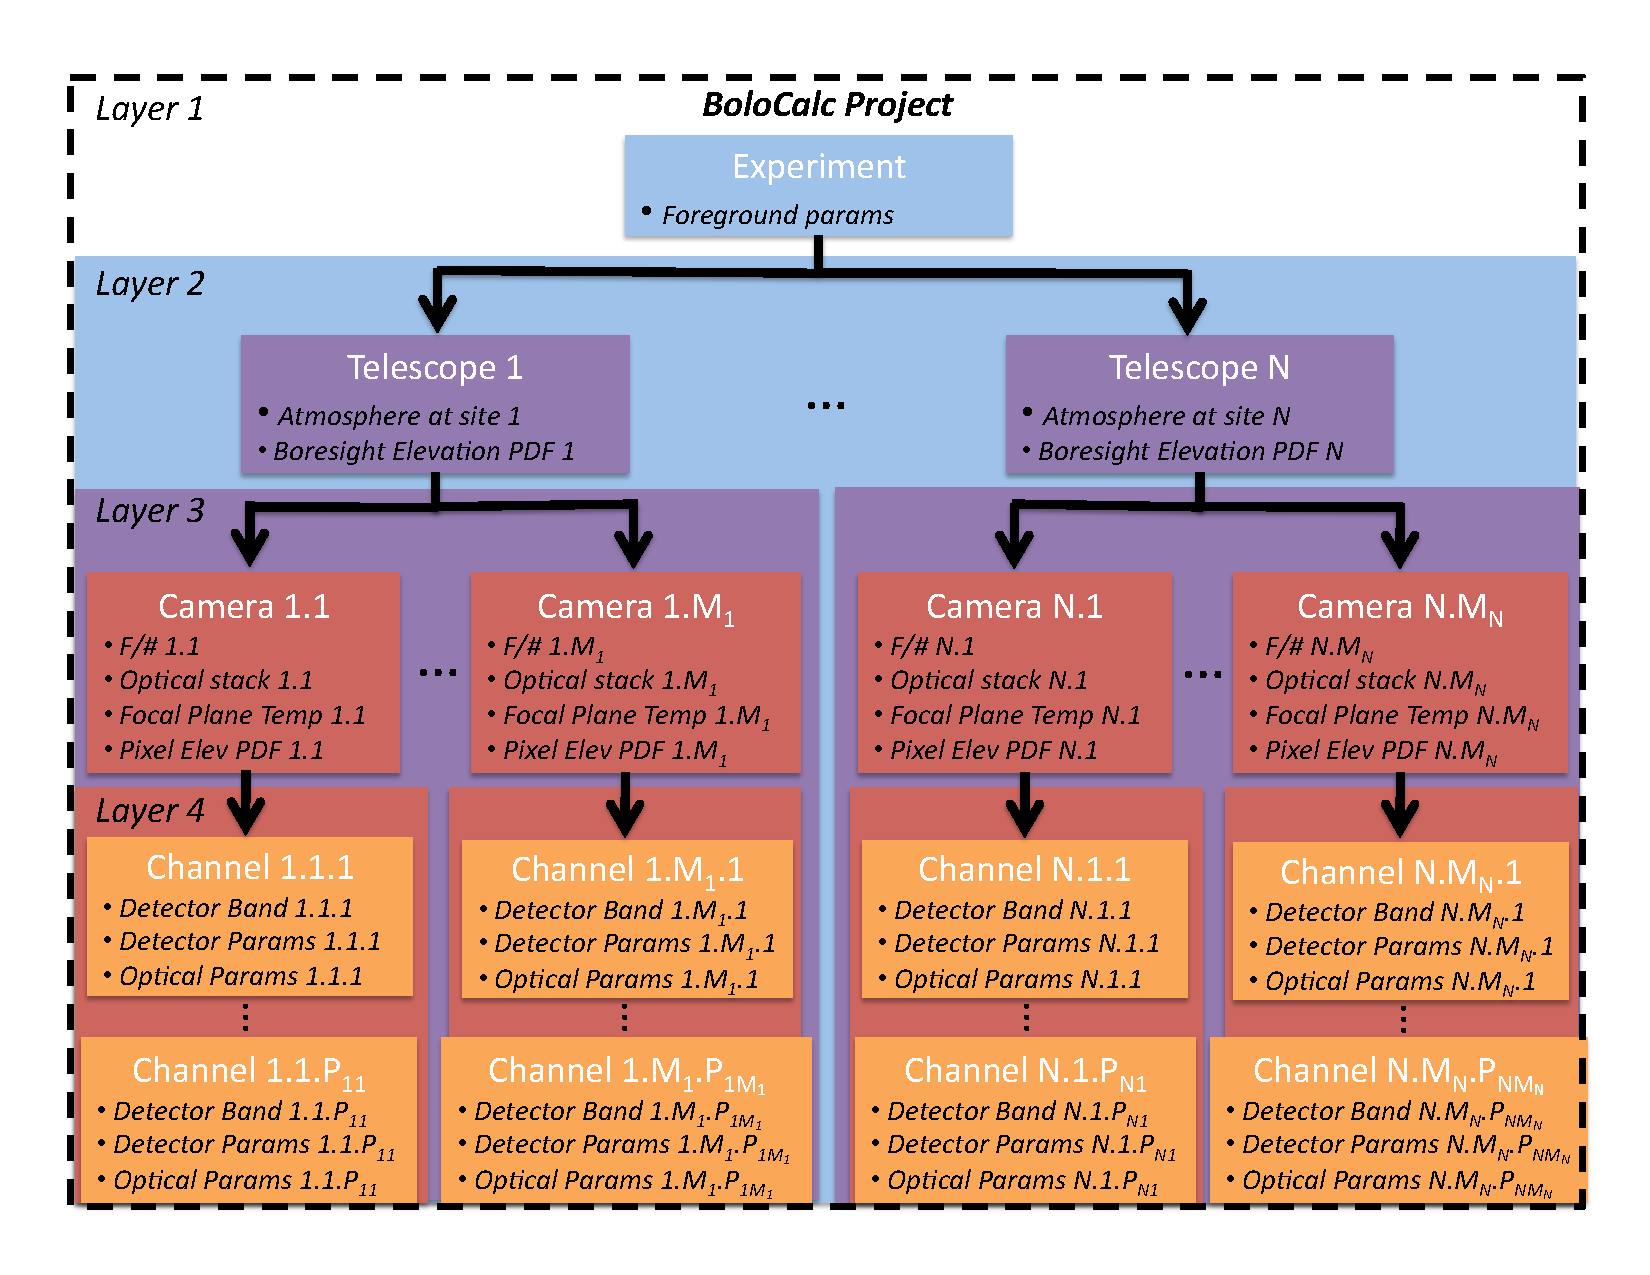
\includegraphics[width=0.98\linewidth]{BoloCalc/Figures/OrgDiagram.pdf}
    \caption[Generic layout of a BoloCalc project]{Generic layout of a BoloCalc project. There are four layers to a project, each with its own set of parameters: (1) experiments, (2) telescopes, (3) cameras, and (4) channels.  There can be an arbitrary set of $N$ telescopes in each experiment, an arbitrary set of $M$ cameras in each telescope, and an arbitrary set of $P$ channels in each camera. Each telescope inherits the parameters of its parent experiment, each camera inherits that of its telescope, and each channel that of its camera. The black bullet points highlight some important parameter definitions that occur within each layer.}
    \label{fig:bolocalc_layout}
\end{figure}

\begin{table}[!ht]
	\centering
    \tabulinesep=0.8mm
	\begin{tabu}[t]{|| l | p{13cm} ||}
    \hline
    \textbf{Layer} & \textbf{Definition} \\
    \hline
    \hline
    Experiment & An assemblage of CMB telescopes. \\
    \hline
    Telescope & A platform that carries and points one or more cameras. It observes at a specified site with a specified observation strategy and can include warm reflectors. \\
    \hline
    Camera & A cryostat that houses cryogenic optics, filters, and detectors. Multiple cameras can be mounted on the same telescope. \\
    \hline
    Channel & A frequency band observed by some set of detectors within a camera. A multichroic camera will have multiple channels. \\
    \hline
    \end{tabu}
    \caption{Definitions of the layers used to build a BoloCalc project.  \label{tab:bolocalc_layers}} 
\end{table}

Table~\ref{table:telescope} shows the user-defined parameters for Layers 1--4 of a BoloCalc project. Layer 1 defines the foreground parameters for each experiment, which determines the celestial optical loading on the detector. While foregrounds contribute little in-band power relative to the atmosphere and CMB at $\sim$~100~GHz, they can become important to an accurate $P_{\mathrm{opt}}$ estimate for satellite experiments that observe at very high and/or low frequencies and therefore are included in BoloCalc for LB and similar missions \cite{litebird_spie_2018}. Layer 2 defines each telescope's atmospheric conditions, as well as its elevation distribution, observation time and efficiency, and sky fraction. Layer 3 defines each camera's optical chain and magnification, as well as its FOV and focal plane temperature. Layer 4 defines the channels within each camera, including the detector parameters, bandpasses, and antenna beam properties. This layered organization allows BoloCalc to seamlessly interface with the Experiment directory structure, which is shown in Figure~blah. 

The BoloCalc source code is composed of 30 classes which form a tree of inheritance with functional branches. Each of these classes serve a very specific function that when instantiated forms an efficient structure which is important for minimizing computation time. Computational efficiency is especially important when running Monte Carlo realizations of the experiment and when running parameter sweeps, which we describe in detail in the sections that follow.

%%%%%%%%%%%%%%%%%%%%%%%%%%%%%%%%
%%%%%%%%%%%%%%%%%%%%%%%%%%%%%%%%

\subsection{Input and output parameters}
\label{sec:bolocalc_input_parameters}

BoloCalc accepts 65 unique input parameters that are used to define all four experiment levels. The parameters are used to describe the foreground emission, the atmosphere and observation strategy, the camera optics, and the detector specifications. These together are used to generate an instrument model that is then simulated to generate the outputs, which are discussed in Section~\ref{sec:bolocalc_output_parameters}. Below is a list of the inputs, organized by level, along with their corresponding symbol in Section~\ref{ch:cmb_instrument_sensitivity}, which describes the sensitivity calculation.  

\noindent
\important{Level 1 parameters}, common to all telescopes in a given experiment:
\begin{itemize}
    \item Foregrounds
        \begin{itemize}
        \item Dust Temperature: $T_{d}$ in Equation~\ref{eq:dust}
        \item Dust Spectral Index: $n_{d}$ in Equation~\ref{eq:dust}
        \item Dust Amplitude: $A_{d}$ in Equation~\ref{eq:dust}
        \item Dust Scale Frequency: $\nu_{d}$ in Equation~\ref{eq:dust}
        \item Synchrotron Spectral Index: $n_{s}$ in Equation~\ref{eq:synch}
        \item Synchrotron Amplitude: $T_{s}$ in Equation \ref{eq:synch}
        \item Synchrotron Scale Frequency: $\nu_{s}$ in Equation~\ref{eq:synch}
        \end{itemize}
\end{itemize}

\noindent
\important{Level 2 parameters}, common to all cameras in a given telescope:
\begin{itemize}
    \item Observation parameters
        \begin{itemize}
        \item Sky Temperature: $T$ in Equation~\ref{eq:planck_spec}
        \item Site: site at which the telescope observes (see Section~\ref{sec:bolocalc_atmosphere}
        \item Elevation: telescope boresight elevation above the horizon
        \item PWV: precipitable water vapor (see Section~\ref{sec:bolocalc_atmosphere}
        \item Observation Time: $t_{obs}$ in Equation \ref{eq:map_depth}
        \item Sky Fraction: $f_{sky}$ in Equation~\ref{eq:map_depth}
        \item Observation Efficiency: $\eta_{obs}$ in Equation \ref{eq:map_depth}
        \item NET Margin: factor applied to all NETs within a telescope, which can be treated as contingency
        \end{itemize}
\end{itemize}

\noindent
\important{Level 3 parameters}, common to all channels in a given camera:
\begin{itemize}
    \item Camera parameters
        \begin{itemize}
        \item Boresight Elevation: boresight elevation of the camera with respect to the telescope boresight
        \item Optical Coupling: $\xi$ in Equations~\ref{eq:trj_fact} and~\ref{eq:tcmb_fact}
        \item F Number: $F$ in Equation~\ref{eq:aperture_eff}
        \item Bath Temp: $T_{b}$ in Equations~\ref{eq:nep_g},~\ref{eq:g}, and~\ref{eq:flink}
        \end{itemize}
\end{itemize}

\noindent
\important{Level 4 parameters}, common to all channels in a given camera:
\begin{itemize}
    \item Channel parameters
        \begin{itemize}
        \item Band Center: $\nu_{c}$ in Equation~\ref{eq:top_hat}
        \item Fractional Bandwidth: $f_{BW}$ in Equation~\ref{eq:top_hat}
        \item Pixel Size: $D_{pix}$ in Equation~\ref{eq:aperture_eff}
        \item Number of detectors per wafer
        \item Number of wafers per optics tube
        \item Number of optics tubes in this camera
        \item Waist Factor: $w_{f}$ in Equation~\ref{eq:aperture_eff}
        \item Detector optical efficiency: $\eta_{det}$ in Equations~\ref{eq:throughput} and~\ref{eq:band_eff_scale}
        \item Bolometer saturation power: $P_{sat}$ in Equations~\ref{eq:g} and~\ref{eq:nep_read}
        \item Psat Factor: $f_{psat}$ in Equation~\ref{eq:psat_fact}
        \item Carrier Index: $n$ in Equations~\ref{eq:g} and~\ref{eq:flink}
        \item Bolometer transition temperature: $T_{c}$ in Equations~\ref{eq:g},~\ref{eq:flink}, and~\ref{eq:nep_g}
        \item Tc Fraction: $f_{\mathrm{c}}$ in Equation~\ref{eq:foper}
        \item Thermal link factor: $F_{link}$ in Equations~\ref{eq:flink} and~\ref{eq:nep_g} \item Dynamic thermal conductance: $G$ in Equations~\ref{eq:g} and~\ref{eq:nep_g}
        \item Detector yield: $Y$ in Equation~\ref{eq:net_arr}
        \item Readout noise: NEI in Equation~\ref{eq:nep_read}
        \item Bolometer operating resistance: $R_{\mathrm{bolo}}$ in Equation~\ref{eq:nep_read}
        \item Responsivity factor: $S_{\mathrm{fact}}$ in Equations~\ref{eq:nep_read},~\ref{eq:responsivity}, and~\ref{eq:readout_responsivity}
        \item Readout noise fraction: $\Delta_{\mathrm{read}}$ in Equation~\ref{eq:frac_nep_read}
        \end{itemize}
    \item Optics parameters
        \begin{itemize}
        \item Temperature: $T_{\mathrm{i}}$ in Equation~\ref{eq:pow_spec_density}
        \item Emissivity/absorptivity: $\epsilon_{\mathrm{i}}$ in Equation~\ref{eq:pow_spec_density}
        \item Reflectivity: $r_{\mathrm{i}}$ in Equations~\ref{eq:popt},~\ref{eq:throughput}, and~\ref{eq:efficiency}
        \item Optical thickness: $t_{\mathrm{i}}$ in Equation~\ref{eq:dielectric_absorption}
        \item Refractive index: $n_{\mathrm{i}}$ in Equation~\ref{eq:dielectric_absorption}
        \item Loss Tangent: $\mathrm{tan} \delta_{\mathrm{i}}$ in Equation~\ref{eq:dielectric_absorption}
        \item Conductivity: $\sigma_{c}$ in Equation~\ref{eq:conductor_absorption}
        \item Surface Roughness: $\sigma_{r}$ in Equation~\ref{eq:ruze_scattering}
        \item Scatter fraction: $\delta_{i}$ in Equation~\ref{eq:pow_spec_density}
        \item Scatter temperature: $T_{\delta ; i}$ in Equation~\ref{eq:pow_spec_density}
        \item Spillover fraction: $\beta_{i}$ in Equation~\ref{eq:pow_spec_density}
        \item Spillover Temperature: $T_{\beta ; i}$ in Equation~\ref{eq:pow_spec_density}
        \end{itemize}
\end{itemize}
Some optics channel parameters are functionally redundant, offering the user multiple methods for calculating emissivity, efficiency, and scattering. For example, the absorptivity of a refractive optic can be entered explicitly, or it can be derived using loss tangent, thickness, and dielectric constant. In a similar manner, there are multiple ways to define certain channel parameters. For example, dynamic thermal conductance $g$ can either be defined explicitly or derived from $T_{\mathrm{c}}$, $T_{\mathrm{b}}$, and $n$. As another example, readout noise can either be defined using NEI, $R_{\mathrm{bolo}}$, and $P_{\mathrm{sat}}$ or it can be stated as a fraction of the detector NEP, offering some flexibility about the level of specificity needed to define its contribution. These flexibilities make BoloCalc useful for a wide range of scenarios, all the way from defining high-level specifications upon project conception to evaluating the impact of low-level measurements during instrument commissioning.

BoloCalc uses the presented input parameters and the equations in Chapter~\ref{ch:cmb_instrument_sensitivity} to calculate 12 \important{output parameters}: 
\begin{itemize}
    \item Optical Throughput: $\eta_{\mathrm{inst}}$ in Equation~\ref{eq:throughput}
    \item Optical Power: $P_{\mathrm{opt}}$ in Equation~\ref{eq:popt}
    \item Telescope Temperature: $T_{\mathrm{tel}}$ in Equation~\ref{eq:tel_temp}
    \item Sky Temperature: $T_{\mathrm{sky}}$ in Equation~\ref{eq:sky_temp}
    \item Photon NEP: $NEP_{\mathrm{ph}}$ in Equation~\ref{eq:nep_ph}
    \item Bolometer thermal NEP: $NEP_{\mathrm{g}}$ in Equation~\ref{eq:nep_g}
    \item Readout NEP: $NEP_{\mathrm{read}}$ in Equation~\ref{eq:nep_read}
    \item Detector NEP: $NEP_{\mathrm{det}}$ in Equation~\ref{eq:nep_det}
    \item Detector NET (CMB or RJ): $NET_{\mathrm{det}}$ in Equation~\ref{eq:net}
    \item Array NET (CMB or RJ): $NET_{\mathrm{arr}}$ in Equation~\ref{eq:net_arr}
    \item Correlation Factor: $\Gamma$ in Equation~\ref{eq:corr_fact}
    \item Map Depth: $\sigma_{\mathrm{s}}$ in Equation \ref{eq:map_depth}
\end{itemize}
These parameters are calculated for each channel in each camera, but the NETs, map depths, and mapping speeds are also combined via inverse-variance weighting (see Equation~\ref{eq:net_inverse_variance_weight}) at the telescope and experiment levels to give a an estimated \textit{total} sensitivity of multiple detector arrays across multiple cameras and telescopes. Median values of the given outputs are displayed in text tables, but histograms of the data are also available when running many MC instrument realizations to inspect the shape of the distributions. This capability is important for accurate forecasting, as NET distributions tend to be skewed and therefore poorly described using Gaussian distributions, even if the input distributions are Gaussian. 

In addition to outputting the sensitivity outputs described in Chapter~\ref{ch:cmb_instrument_sensitivity}, BoloCalc generates tables of optical power and optical throughput as a function of location within the camera's optics chain. An example of such a table is shown in Figure~blah. This functionality is quite useful for understanding the propagation of optical power through the telescope system and for identifying which areas of the experiment should receive the most attention when trying to improve $\mathrm{NEP_{ph}}$.

%%%%%%%%%%%%%%%%%%%%%%%%%%%%%%%%
%%%%%%%%%%%%%%%%%%%%%%%%%%%%%%%%

\subsection{User interface}
\label{sec:bolocalc_user_interface}

There are two ways to interact with BoloCalc. The first, which has been utilized throughout most of the calculator's lifetime, is through the command line. In this scheme, experiment inputs are set by directly modifying text tables, and outputs are also generated in text tables. There is the a class that loads the outputs in dictionaries, which can in turn be easily unpacked, plotted, and manipulated in a friendly environment, such as that of a Jupyter Notebook. While this first scheme is well-tested and completely self-sufficient, it is cumbersome at times and sets a barrier to entry for new users. Additionally, as is always the case with Python, errors in user inputs are not assessed until execution, and while BoloCalc logging and error tracing is both well developed and comprehensive, the burden of debugging at the command line can be a deterrent for casual users. Therefore, we have also developed a graphical user interface (GUI) using PyQt named \important{BoloCalc GUI} (BCG).

\begin{figure}
    \centering
    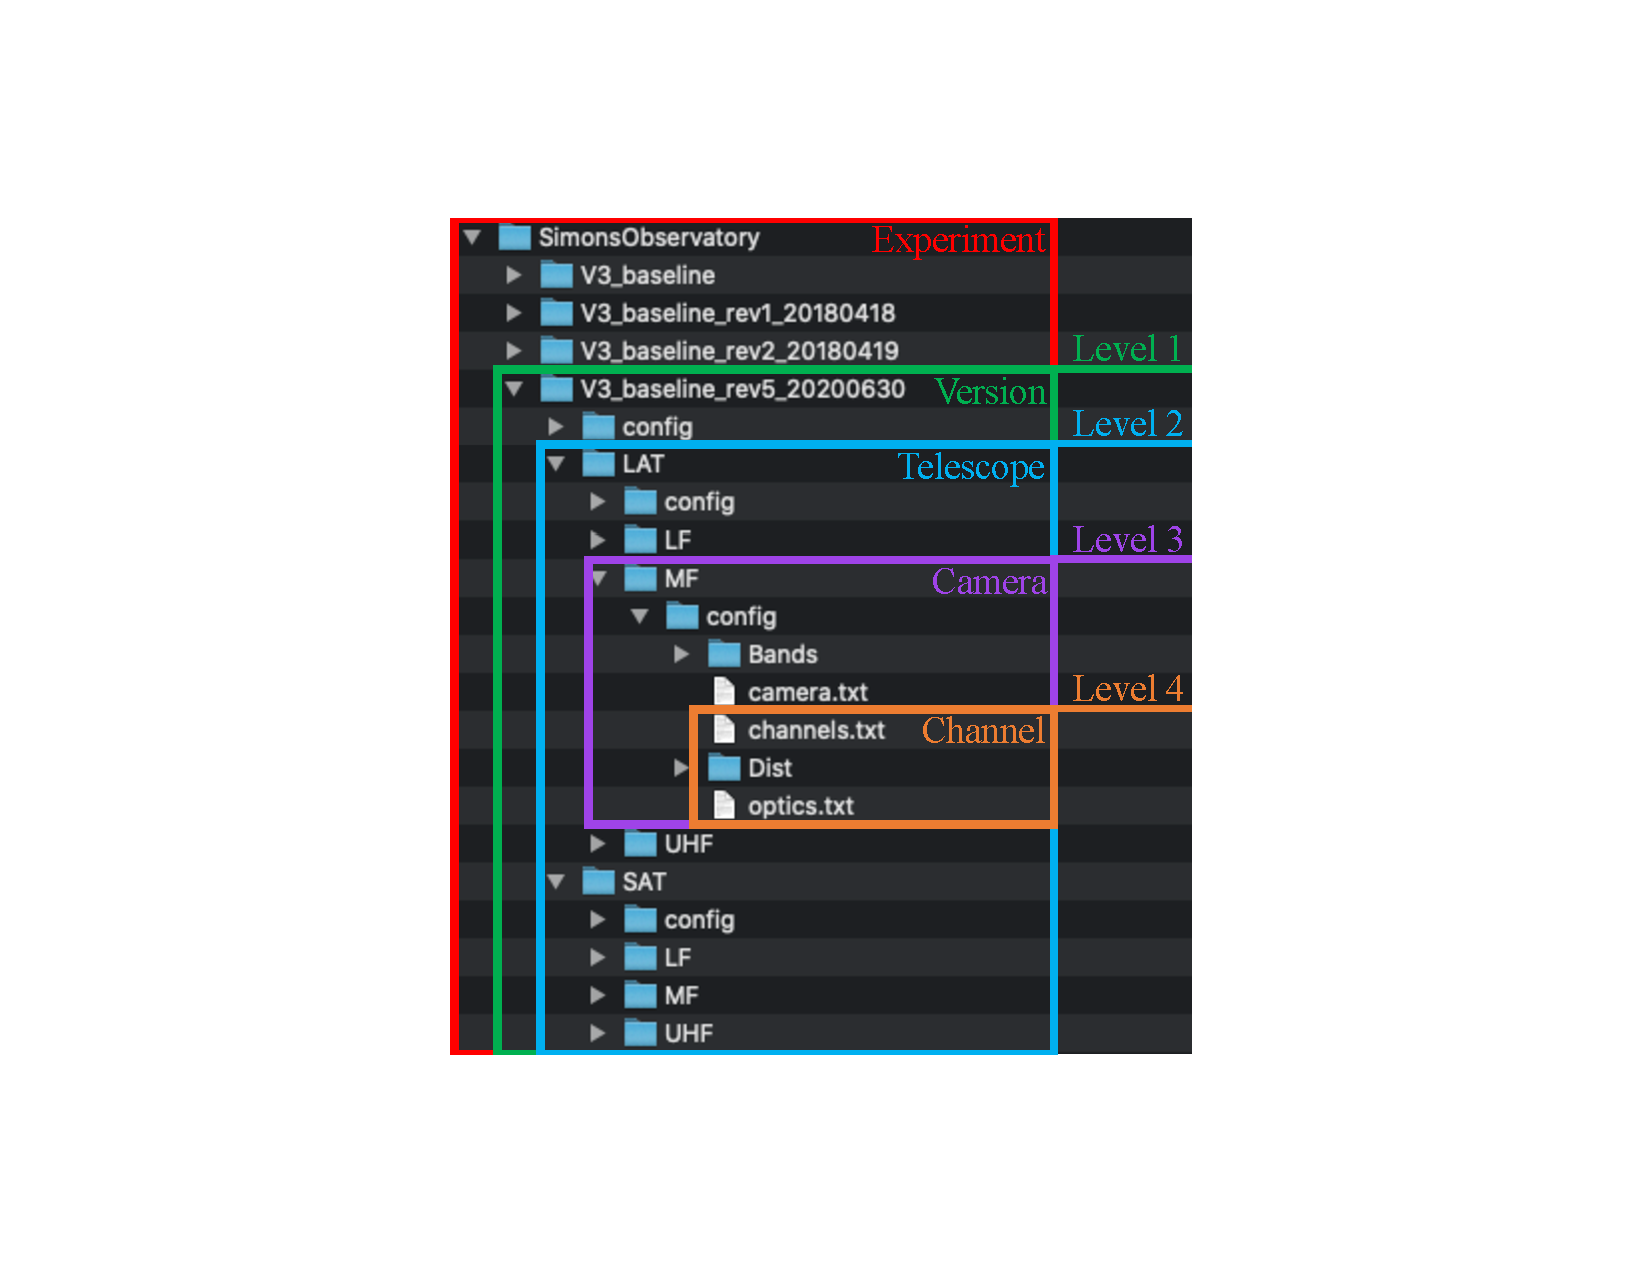
\includegraphics[width=0.8\linewidth, trim=6cm 3.4cm 6cm 3.4cm, clip]{PolarizationModulation/Figures/bolocalc_file_structure.pdf}
    \caption{BoloCalc file structure, showing how the file layout mimics the underlying class structure. This layout is modular, making it straightforward to update experiment versions, add telescopes and cameras, and visualize how the various sybsystems fit together.}
    \label{fig:bolocalc_file_layout}
\end{figure}

The GUI substantially improves the BoloCalc user experience in several ways. First, it removes the need for the user to interact with the command line and use text editors. Because BoloCalc has so many inputs, especially those of the optics (described in Section~\ref{sec:sensitivity_optical_power}), text files can be cumbersome to maintain. BCG acts as a wrapper around the input text files, allowing the user to modify parameters using line edits, combo boxes, and check boxes before saving them into the text files. In addition, BCG performs real-time error checking on user input and uses sub windows to control what inputs the user is allowed to enter. This transfers the error checking of inputs to the front end (when they are entered) as opposed to the back end (during Python interpreter operation). In other words, BCG's function to make sure that when the user runs the code, it's guaranteed to work. Second, BCG has embedded descriptions of input and output parameters in said parameter's edit window. This increases the transparency of the sensitivity calculation and provides immediate information about what outputs each parameter influences. While the BoloCalc user manual does lay out the equations in Section~\ref{ch:cmb_instrument_sensitivity} and clearly show which text-file parameter corresponds to which mathematical symbol, it is cumbersome to manage both the manual and the command prompt simultaneously, again acting as a barrier to more casual users. BCG's in-window definitions fix this issue and also act as a pedagogical tool to increase awareness around how the sensitivity calculation works.

\begin{figure}
    \centering
    \subfloat[\label{fig:bcg:a}]{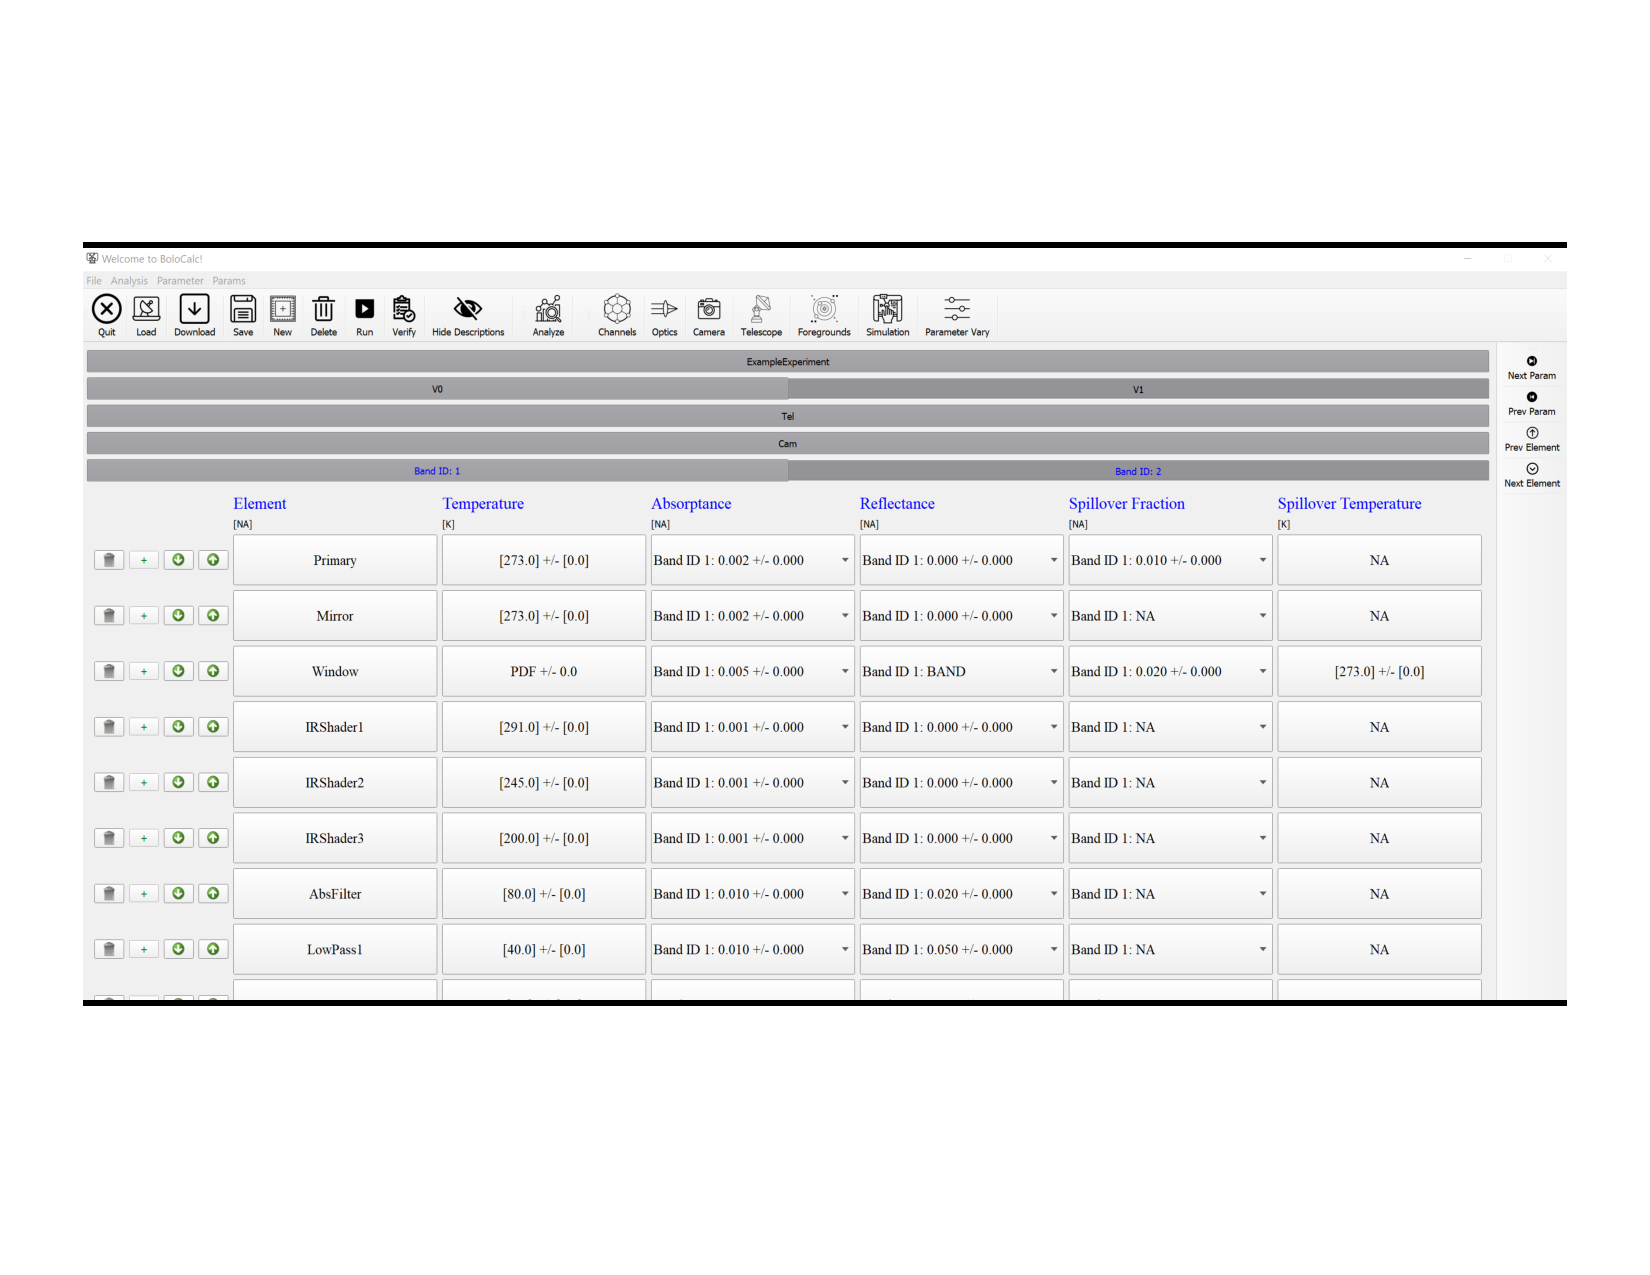
\includegraphics[width=0.8\linewidth, trim=1cm 4cm 1cm 4cm, clip]{BoloCalc/Figures/bcg_optics.pdf}}
    \hfill
    \subfloat[\label{fig:bcg:b}]{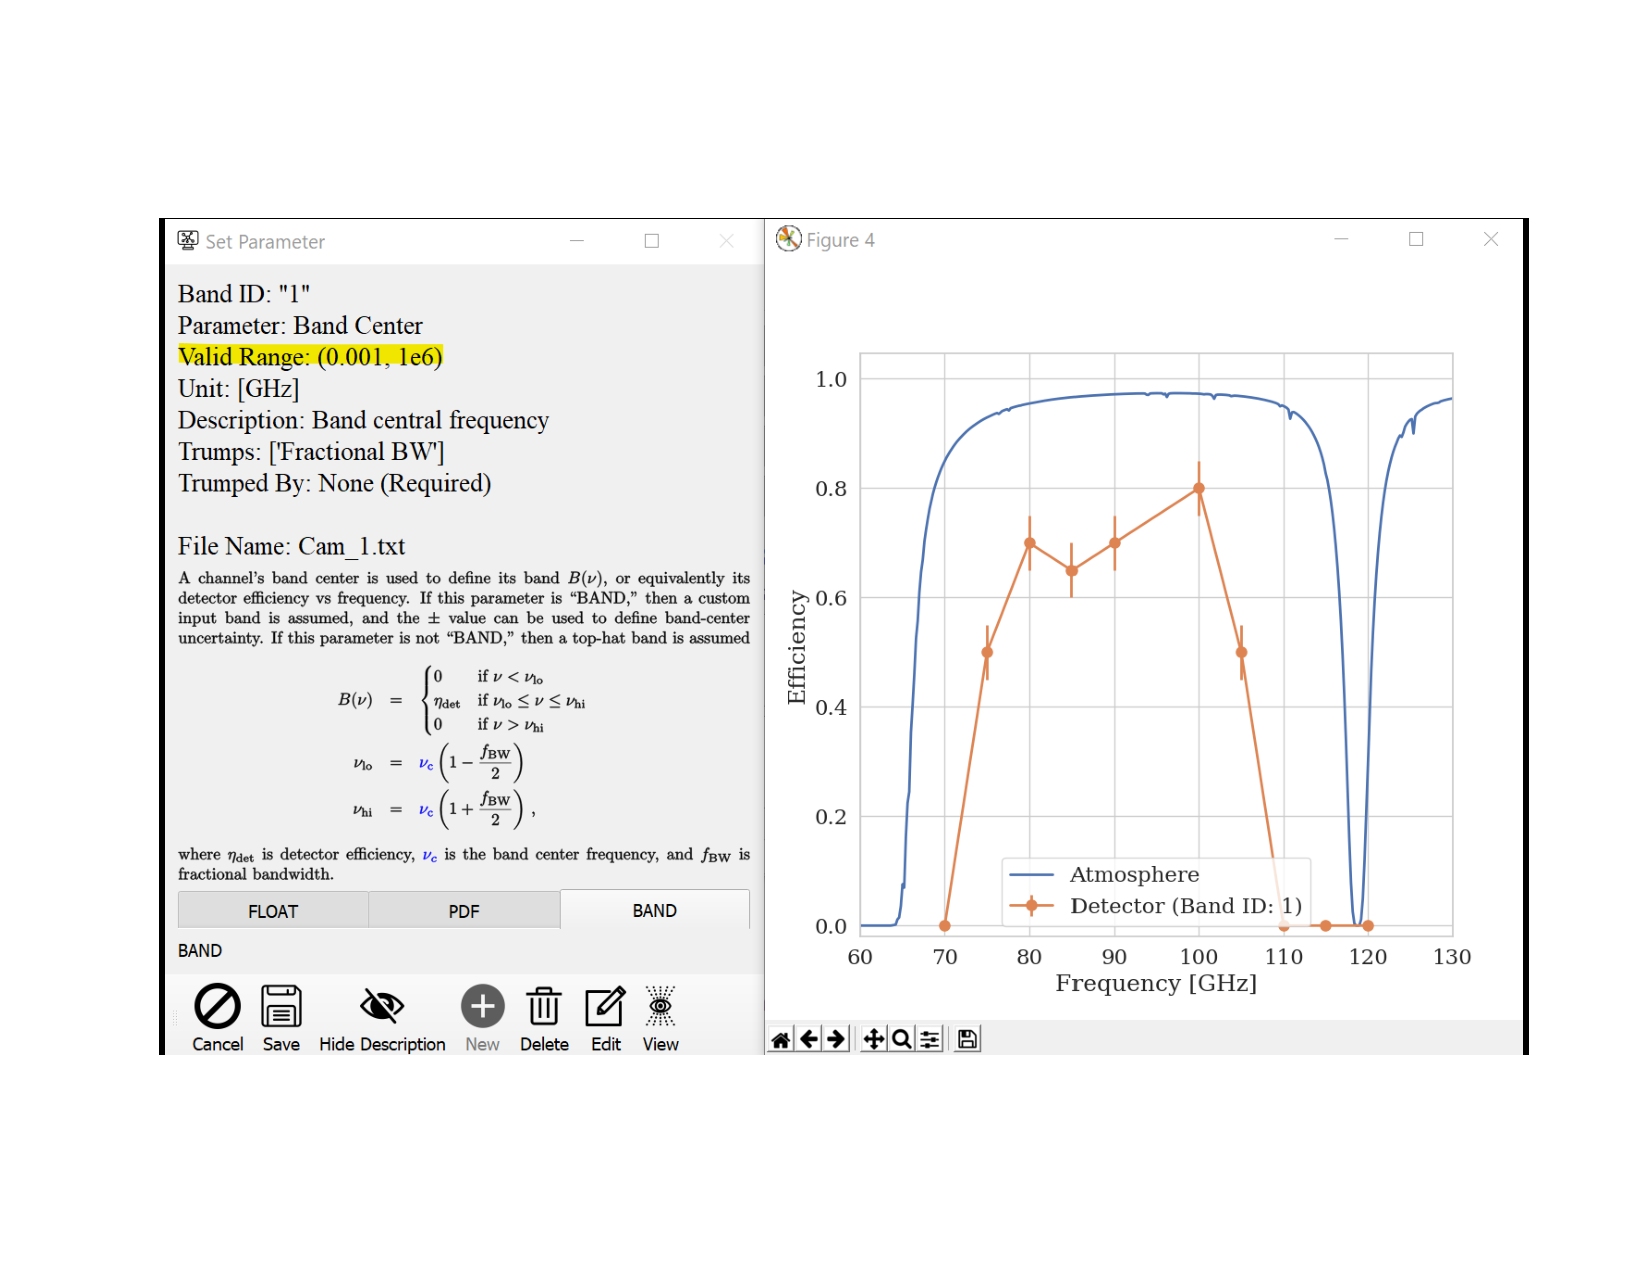
\includegraphics[width=0.8\linewidth, trim=2.1cm 3.5cm 1.9cm 3.5cm, clip]{BoloCalc/Figures/bcg_band.pdf}}
    \caption{Two example of the BoloCalc GUI interface. (a) shows the toolbar for navigating between telescopes, cameras, and channels, and it shows a the table interface for editing optical parameters. The drop-down menus allow the values for each channel to be edited independently. (b) shows an example }
    \label{fig:bcg}
\end{figure}

Third, BCG provides real-time data visualization, both of inputs and, after running the code, the outputs. For example, BCG allows the user to view plots of input probability distributions for parameters, as well as bandpass functions for optics and detectors overplotted onto the assumed atmospheric profile. These functionalities provide immediate, informative feedback to the user on the instrument model and allows for rapid assessments of the assumed inputs by collaborators. The outputs can be either downloaded for plot generation by separate scripts, or they can be plotted with somewhat limited options directly in the UI. In a similar way to with the inputs, this allows for a quick assessment of simulation results even facilitates rapid compilation of documentation and presentations. Fourth, BCG effectively separates the BoloCalc code from the user interface, which is enormously useful for development purposes. Any changes in the underlying text files or source code are decoupled from the user, improving backwards compatibility and making the upgrade process more seamless. 

The most important goal of BCG is to make BoloCalc more accessible to wider range of potential users. During instrument design and development, many scientists are evaluating many aspects of a given instrument in parallel, and in the predominant workflow model, if they want feedback on the impact of their measurement on sensitivity, they must go through the collaboration's sensitivity expert, who is typically the one who wrote and manages that collaboration's sensitivity code. This is a barrier-to-entry problem that should be reduced by BCG for ongoing and future experiments, such as SO and CMB-S4, and we hope that whenever anyone from an undergrad to a principal investigator wonders how parameter X impacts output Y, they can quickly use BoloCalc via BCG to assess their curiosity.


%%%%%%%%%%%%%%%%%%%%%%%%%%%%%%%%
%%%%%%%%%%%%%%%%%%%%%%%%%%%%%%%%
%%%%%%%%%%%%%%%%%%%%%%%%%%%%%%%%

\section{Calculator features}
\label{sec:bolocalc_features}

BoloCalc has several features that distinguish it from its predecessor sensitivity codes. A strength of BoloCalc's object-oriented structure is that it is easy to upgrade and modify, and therefore many of the following subsections are the result of collaboration needs that have arisen throughout BoloCalc's lifetime.

%%%%%%%%%%%%%%%%%%%%%%%%%%%%%%%%
%%%%%%%%%%%%%%%%%%%%%%%%%%%%%%%%

\subsection{Site and atmosphere}
\label{sec:bolocalc_site_atmosphere}

BoloCalc uses atmosphere transmissivity and temperature vs. frequency when calculating $P_{\mathrm{opt}}$. Such a spectrum is often called an \important{atmospheric profile} and depends on the details of the observation site, including elevation above sea level, weather patterns, and sky access. There are three ways in which the atmosphere can be defined in BoloCalc: a constant temperature and transmissivity vs. frequency, a custom profile, and simulated profile selected via PWV and horizon elevation. In this section, we want to highlight the final method, which typically both most informative and accurate.

BoloCalc uses atmospheric profiles generated using the \important{AM atmospheric simulation code} developed at Harvard. AM is a \ct{C++} command-line tool which takes a configuration file that contains the details of the molecular composition of atmosphere at a given observation site. BoloCalc uses atmospheric profiles for three different observation sites: the Atacama, the South Pole, and the stratosphere, from where balloon-borne experiments typically observe. Atmospheric configurations for BoloCalc were provided by Denis Barkats and Scott Paine, and their mm-wave behavior has been compared to sky-temperature measurements of the South Pole Telescope and the Atacama Cosmology Telescope, showing excellent agreement. 

A side-by-side comparison of the assumed atmospheric configurations are shown in Figure~blah, and there are a few aspects to these files that are worth pointing out. (Talk a bit about the various assumptions and components here).

In order to offer ready access to the atmospheric profiles, BoloCalc includes an HDF5 file containing spectra over [0.1, 0.2, ... 1,000]~GHz for all three sites over a PWV range of [0, 0.1, ..., 8]~mm and over an elevation range of [0, 1, ..., 90]~deg above the horizon. Then, when the user defines the Layer 2 parameters \textit{site}, \textit{elevation}, and \textit{PWV}, BoloCalc accesses the corresponding profile using the Python class \ct{h5py}. The HDF5 construction is ideal for this functionality, as it offers fast look-up access to the atmospheric profiles without having to load them into memory. The quick access becomes even more important when running MC realizaions of the sky (see Section~\ref{sec:bolocalc_monte_carlo}).

Note that BoloCalc does not make any simplifying assumptions about how the atmospheric loading changes with elevation or PWV. However, as Figure~blah shows, the approximations are reasonable at low frequencies and low PWV and elevation. 

%%%%%%%%%%%%%%%%%%%%%%%%%%%%%%%%
%%%%%%%%%%%%%%%%%%%%%%%%%%%%%%%%

\subsection{Monte Carlo simulations}
\label{sec:bolocalc_monte_carlo}

From forecasting an instrument's scientific impact to measuring its performance in the field, there will always be uncertainties surrounding the sensitivity estimate, and quantifying these uncertainties is critical to every stage of the experiment. For example, when iterating on high-level design concepts during early stages, there will naturally be enormous error bars surrounding back-of-the-envelope calculations and crudely modeled simulations, and understanding how these uncertainties propagate to NET can inform how to formulate a proposal with adequate resource allocations, contingency scenarios, and properly calibrated science objectives. As an example on the other end of the spectrum, when using planet observations in the field to characterize the responsivity of the detectors, it is important to quantify measurement uncertainties, variations across the focal plane, and modelling limitations so as to not misinterpret the telescope's capabilities. Given the importance of uncertainty modeling, BoloCalc uses MC simulations of the instrument to generate histograms of output parameters.

BoloCalc accepts either a mean and standard deviation or a custom probability density for every input parameter. For custom spectral bands (see Section~\ref{sec:bolocalc_custom_bands}), every data point can be defined by a mean and standard deviation, and distributions in PWV and elevation correspond to an uncertainty in the atmospheric profile (see Section~\ref{sec:bolocalc_site_atmosphere}). BoloCalc breaks MC simulations into three levels: (1) realizations of the foregrounds, telescope, camera, and optics, (2) realizations of the sky, and (3) realizations of the detector parameters. The number realizations are defined separately for each level, meaning that for each of $N$ experiments, $M$ skies, are generated, and for each of $M$ skies, $P$ detectors are generated. Separating the simulation into these three categories is chronologically intuitive: (1) you build and field a telescope which after deployment is relatively static, and then (2) you observe with that telescope in a variety of sky conditions, and then (3) given the sky conditions, you calibrate detector operating parameters. Perhaps more importantly, this division is computationally efficient, as it allows the layers shown in Figure~\ref{fig:bolocalc_layout}) to be simulated from the top down.

In its current form, BoloCalc does not offer any functionality for defining correlated errors. Doing so in a general way would require the user to interact with a large correlation matrix, which is a substantial development project. Such a capability would be particularly useful for quantities whose fluctuations are obviously correlated, like temperatures of optical elements, which depend on the cryostat performance, or the waist factor of detectors in different channels, which share the same optical coupling element on multichroic detector pixels. To counteract this deficiency, BoloCalc offers a comprehensive parameter sweep functionality, which can be used to calculate input-output covariances manually.

%%%%%%%%%%%%%%%%%%%%%%%%%%%%%%%%
%%%%%%%%%%%%%%%%%%%%%%%%%%%%%%%%

\subsection{Parameter sweeps}
\label{sec:bolocalc_parameter_sweeps}

What most clearly separates BoloCalc from its predecessors is its parameter sweep functionality. When defining instrument specifications, it is critical to understand the derivatives of NET vs. various instrumental performance metrics. The scope of useful parameter-sweep studies is very large, and therefore BoloCalc's functionality is completely general in an effort to handle a wide variety of common inquiries such as NET vs. elevation, photon NEP vs. primary spillover, and readout NEP vs. saturation power.

BoloCalc allows you to simulate any sweep across any set of parameters across any of the channels in the experiment. There is an option to either calculate all possible permutations of the parameter sweeps or to sweep over them together, and the input vector can either be defined with linear spacing or passed via a custom input file. MC simulations can also be carried out for each parameter set, allowing the user to inspect not only how a parameter sweep changes the mean/median NET but also how it might change the shape of its distribution.

Parameter sweeps, especially when combined with MC simulations, can be computationally expensive, and therefore substantial effort has been put towards ensuring that BoloCalc sweeps are performed efficiently. To do this, an ``initial'' experiment realization is constructed, and as each parameter is changed, only the affected instrument aspects are resimulated. For example, if the user changes the detector optical efficiency of a 90~GHz bolometer in Camera~1, only the MC realizations of the 90~GHz detectors in Camera~1 are recalculated, while the the other channels (e.g. 150~GHz), the telescope optics, and all other cameras and telescopes are left untouched. However, if the spillover fraction of the telescope's primary mirror is varied, then all of the cameras and detectors in that telescope are recalculated, while other telescopes are left untouched. This top-down scheme enables for rapid iteration over many parameters on a time scale of minutes, even when simulating thousands of instrument realizations. 

The parameters sweep output files are carefully constructed for friendly inspection, and an \ct{output.py} class loads these files into dictionaries for easy plotting. In addition, BCG contains a comprehensive system of comboboxes that allows the user to plot any output vs. an arbitrary combination of input parameters, enabling even quicker and easier feedback to instrument designers.

%%%%%%%%%%%%%%%%%%%%%%%%%%%%%%%%
%%%%%%%%%%%%%%%%%%%%%%%%%%%%%%%%

\subsection{Custom bandpasses}
\label{sec:bolocalc_custom_bands}

BoloCalc offers two ways to handle \important{bands}, or input parameters that vary with frequency, such as absorptivity, transmissivity, reflectivity, spillover fraction, and scattering fraction. The first method is define a \important{top-hat band}
\begin{equation}
    B ( \nu) = 
    \begin{cases}
        0    & \text{if } \nu < \nu_{\mathrm{lo}} \\
        \alpha(\nu) & \text{if } \nu_{\mathrm{lo}} \leq \nu \leq \nu_{\mathrm{hi}} \\
        0    & \text{if } \nu > \nu_{\mathrm{hi}} \, ,
    \end{cases}
    \label{eq:bolocalc_tophat_band}
\end{equation}
where $\alpha(\nu)$ is, in general, a function of frequency and where the band edges $\nu_{\mathrm{lo}}$ and $\nu_{\mathrm{hi}}$ are defined by discontinuities. The most common top-hat band is when $\alpha(\nu) = \mathrm{const.}$, giving rise to a rectangular window function. The top-hat band definition is convenient because its spectral extent is defined by only band center $\nu_{\mathrm{c}}$ and fractional bandwidth $f_{\mathrm{BW}}$
\begin{align}
    \nu_{\mathrm{lo}} = \nu_{\mathrm{c}} - \frac{ \nu_{\mathrm{c}} \, f_{\mathrm{BW}}}{2} \label{eq:band_lo} \\
    \nu_{\mathrm{hi}} = \nu_{\mathrm{c}} + \frac{ \nu_{\mathrm{c}} \, f_{\mathrm{BW}}}{2} \label{eq:band_hi} \, ,
\end{align}
making the estimate of band-averaged quantities algebraically trivial.

In reality, bands have spectral features that arise due to any number of physical factors. For example, in an optical element, \important{Fabry-Perot} fringes in transmissivity appear due to peaks/troughs of maximum constructive/destructive interference. For another example, ripples develop in detector bands due to internal reflections between on-chip capacitors used to define the band itself. Also, bands in general have a roll-off that is not infinite, and the shape of this roll-off can be important for understanding the impact of, for example, atmospheric lines on $P_{\mathrm{opt}}$. For these reasons and more, BoloCalc accepts custom input bands (in either TXT or CSV format), with both mean parameter value and standard deviation over an array of frequencies. An additional feature is that BoloCalc also allows the band centers of these input bands to be either swept or assigned an uncertainty during MC simulations. Band center uncertainty is a major component of detector fabrication, and therefore this features has proven to be valuable for detector characterization and design feedback.

The frequency resolution of any BoloCalc simulation can be tuned to $\Delta f \geq 0.1$~GHz, offering the user another lever to optimize computation time vs. accuracy. For example, if a lab measurement of an optical element is performed with high frequency resolution, the user can opt to also run the BoloCalc simulation with high frequency resolution to best capture the impact of the optic measurement on NET. In the other limit, if the user is using band with minimal features (such as top-hats) but wants to run hundreds of thousands of simulations to best quantify the influences of measurement uncertainties, they can increase the frequency resolution to maintain a reasonable computation time. 

%%%%%%%%%%%%%%%%%%%%%%%%%%%%%%%%
%%%%%%%%%%%%%%%%%%%%%%%%%%%%%%%%
%%%%%%%%%%%%%%%%%%%%%%%%%%%%%%%%

\section{Calculator validation}
\label{sec:bolocalc_validation}

In 2014, BoloCalc was born to forecast NETs for LiteBIRD in order to inform the design of its detector arrays. In order to ensure its accuracy, the sensitivity code was checked against that of LiteBIRD's Japanese team, and all outputs were confirmed to be identical for a variety of input assumptions. During the same period, several sets of output parameters vs. input parameter sweeps were compared against legacy codes, such as those of POLARBEAR-2 (Aritoki Suzuki) and SPT-SZ (Nils Halverson) to ensure that mapping speed limits and scalings were consistent.

In 2016, during the early stages of SO, BoloCalc was further compared against sensitivity codes from ACT (Suzanne Staggs and Sarah Marie Bruno) to ensure that relative mapping speed scalings were consistent across many different parameters. This comparison was especially critical during this early period of calculating mapping speed vs. cost for a plethora of instrument configurations, some of which are discussed in Section~\ref{sec:bolocalc_informing_so_design}.

Shortly thereafter, as SO's instrument design matured and its science forecast paper was being actively worked on, BoloCalc models were built for POLARBEAR, ACTpol, Advanced ACTpol, and ABS, all of which have published array NETs against which the BoloCalc prediction were compared. This comparison covered a wide variety of frequencies from 30~GHz to 270~GHz and multiple detector, optical, and telescope infrastructures. For each case, the achieved array NET was within $1 \sigma$ of BoloCalc's median expectation, inspiring confidence that the calculator is indeed detailed and accurate enough to predict and characterize actual instrument performance. This final comparison is very important to the validity of the calculator for the broader CMB community, especially CMB-S4, and therefore we plan to publish our findings in an upcoming paper.

%%%%%%%%%%%%%%%%%%%%%%%%%%%%%%%%
%%%%%%%%%%%%%%%%%%%%%%%%%%%%%%%%
%%%%%%%%%%%%%%%%%%%%%%%%%%%%%%%%

\section{Informing the design of SO}
\label{sec:bolocalc_informing_so_design}

One of BoloCalc's primary applications has been to inform the design and development of SO. During SO's earliest stages, there were a menagerie of open questions about the instrument design. In order to make progress, SO needed an efficient feedback loop between the science team---which studies SO science targets and the needed map depths to achieve them---and the instrument team---which translates the science team's recommendations into an observatory concept and assess its technological feasibility and cost. During these early stages, BoloCalc was a crucial ``glue'' that bound these discussions together by calculating the NET of a given instrument design. In this section, we discuss some of BoloCalc's most important SO design studies both to showcase the calculator's utility and to highlight it's contributions to the resulting SO design. 

The SO design is discussed as part of Chapter~\ref{ch:cmb_instrument_overview}, but we review the basics here before diving into details. SO uses dichroic pixels and distributes its frequency bands between 27/39~GHz ``low-frequency'' (LF) pixels, 90/150~GHz ``mid-frequency'' (MF) pixels, and 220/270~GHz ``ultra-high-frequency'' (UHF) pixels. Lenslet-coupled sinuous antennas are baselined for the LF wafers, while a feedhorn and OMT architecture is baselined for the MF and UHF wafers. The wafers are distributed between cameras in the LAT, which each house three wafers\footnote{The LAT cameras have a FOV that can accommodate up to 4~wafers, allowing for future upgrades.}, and the SATs, which each house seven wafers.

%%%%%%%%%%%%%%%%%%%%%%%%%%%%%%%%
%%%%%%%%%%%%%%%%%%%%%%%%%%%%%%%%

\subsection{LATR architecture}
\label{sec:bolocalc_latr_design}

The LAT is the vehicle for SO's high-$\ell$ science, and its goal is to achieve arcminute resolution in 6 frequency bands from 30~GHz to 280~GHz across an 8~deg FOV. In order to achieve this goal, both the telescope and receiver need to be quite large and are therefore huge cost drivers. For this reason, among others, the LAT system was designed top-down, with the telescope design driving that of the LATR, which drove that of the optics tubes, which drove that of the detector arrays. Of course there was iteration and interaction among the teams that designed each subsystem, and the much of the optimization ran both ways, but for the LAT discussions to follow, much of the larger elements are held constant while the smaller elements are optimized.

The LAT has a field of view of $7.8^{\circ}$ that illuminates a 2.5~m diameter area at the telescope's focus. At this point, it is the job of the LATR to reimage the telescope image onto detector arrays. An early application of BoloCalc was to help determine how many optics tubes to deploy in the LATR. This question involves a complex mixture of telescope optics, cryo-vacuum engineering, mechanical design and assembly, reimaging optics, cost, and upgradability, 
%\cite{galitzki_so_2018,gallardo_lat_2018,orlowski-sherer_latr_2018,zhu_latr_2018,dicker_lat_2018}
but evaluating sensitivity was central to the decision making process.

Figure~\ref{fig:so_ot_configs} shows a study of three different optics-tube configurations that were considered for the LAT. This particular investigation involved a fixed telescope FOV and hexagonal camera packing. Config A has 19 ``small-diameter'' cameras with a maximum of one wafer per camera, Config B has 13 ``medium-diameter'' cameras with a maximum of four wafers per camera, and Config C has 7 ``large-diameter'' cameras with a maximum of seven wafers per camera. Pixel size was held constant and F-number (F/\#) varied with plate scale to maximize each camera's FOV.
%For more detail regarding the LAT optimization, see Dicker \textit{et al.} \cite{dicker_lat_2018}.

Each configuration impacts each camera subsystem (e.g. detectors, refractive optics, cryogenics, etc.) differently, but Fig.~\ref{fig:so_ot_configs:b} shows the relative maximum-achievable MS for each arrangement across all six frequency bands. As shown, Config B has the best overall MS at LF and MF, with only a marginal MS degradation at UHF. Driven in part by this MS calculation, Config B was chosen as the LATR architecture.

\begin{figure}[!t]
    \subfloat[\label{fig:so_ot_configs:a}]{
        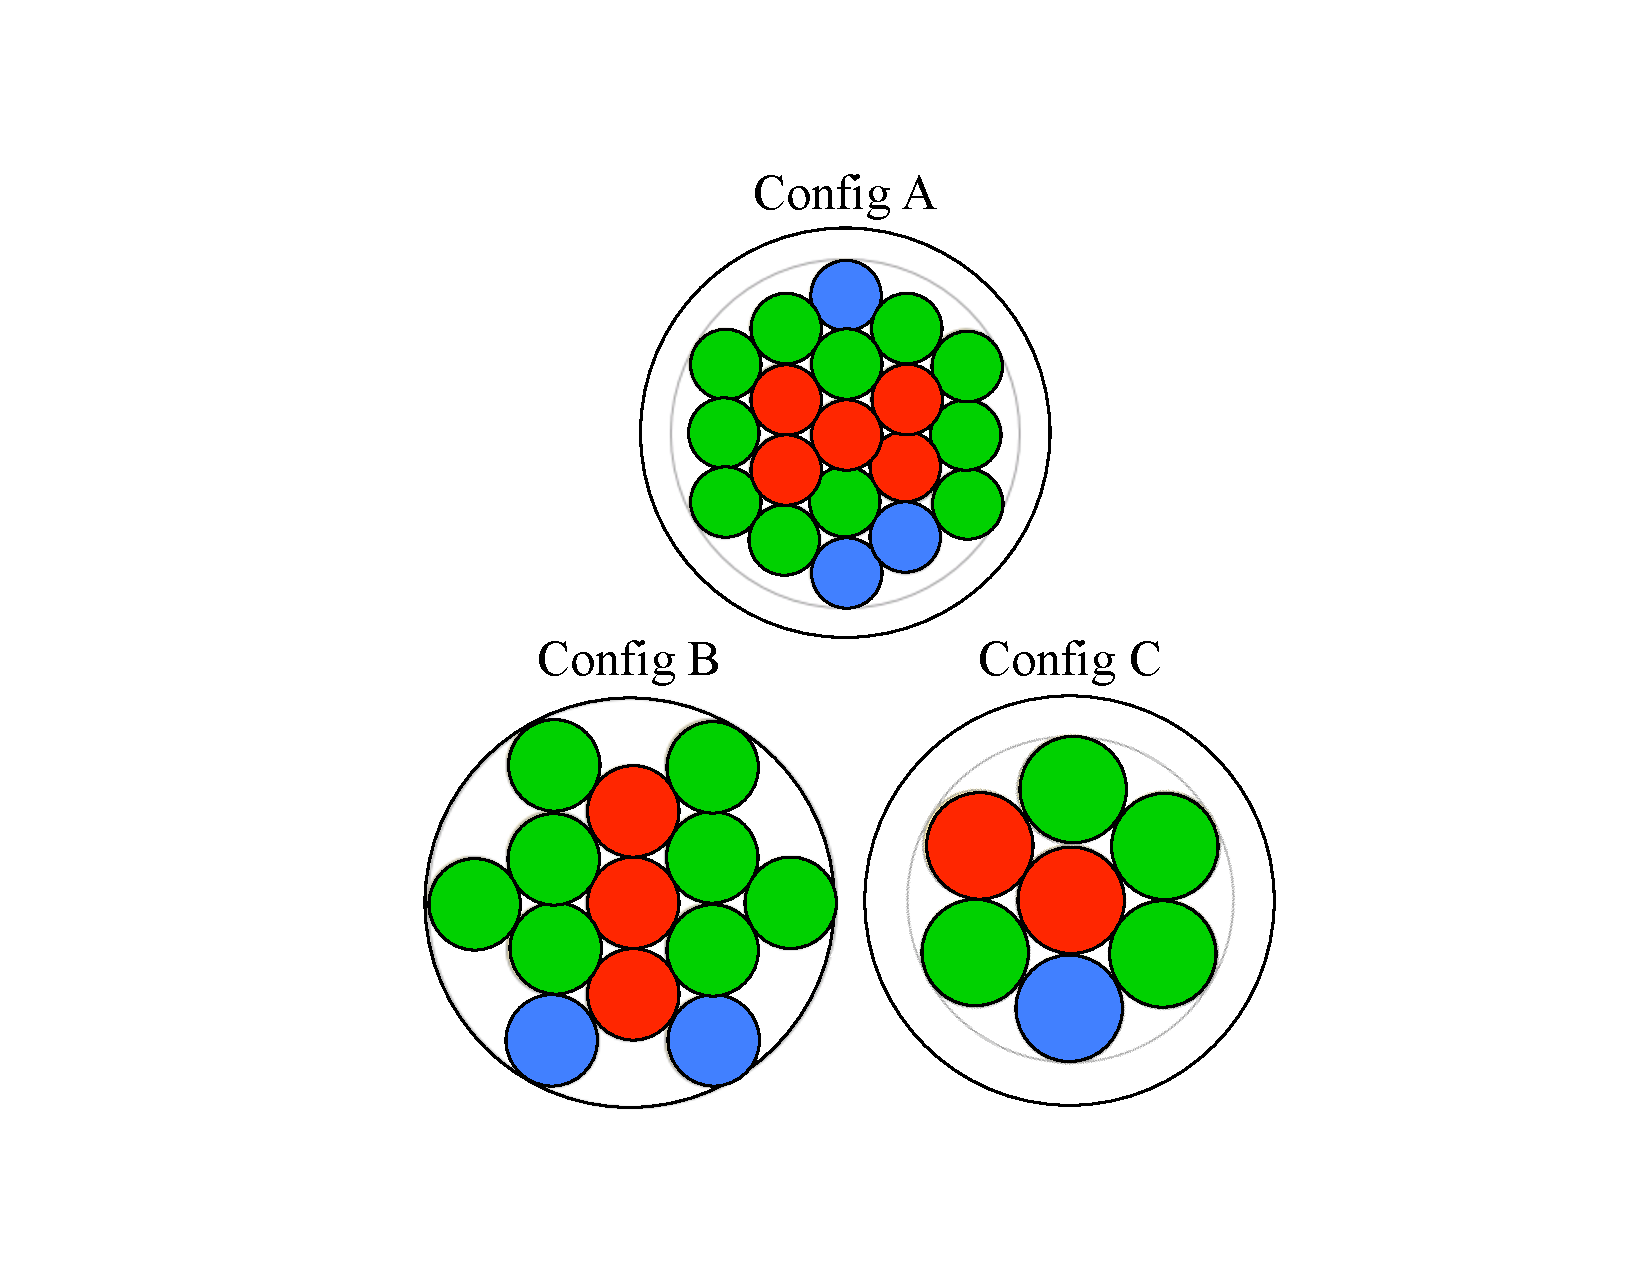
\includegraphics[width=0.4\linewidth, trim=6cm 2cm 6cm 2.9cm, clip]{BoloCalc/Figures/StackedConfigs.pdf}
    }
    \subfloat[\label{fig:so_ot_configs:b}]{
        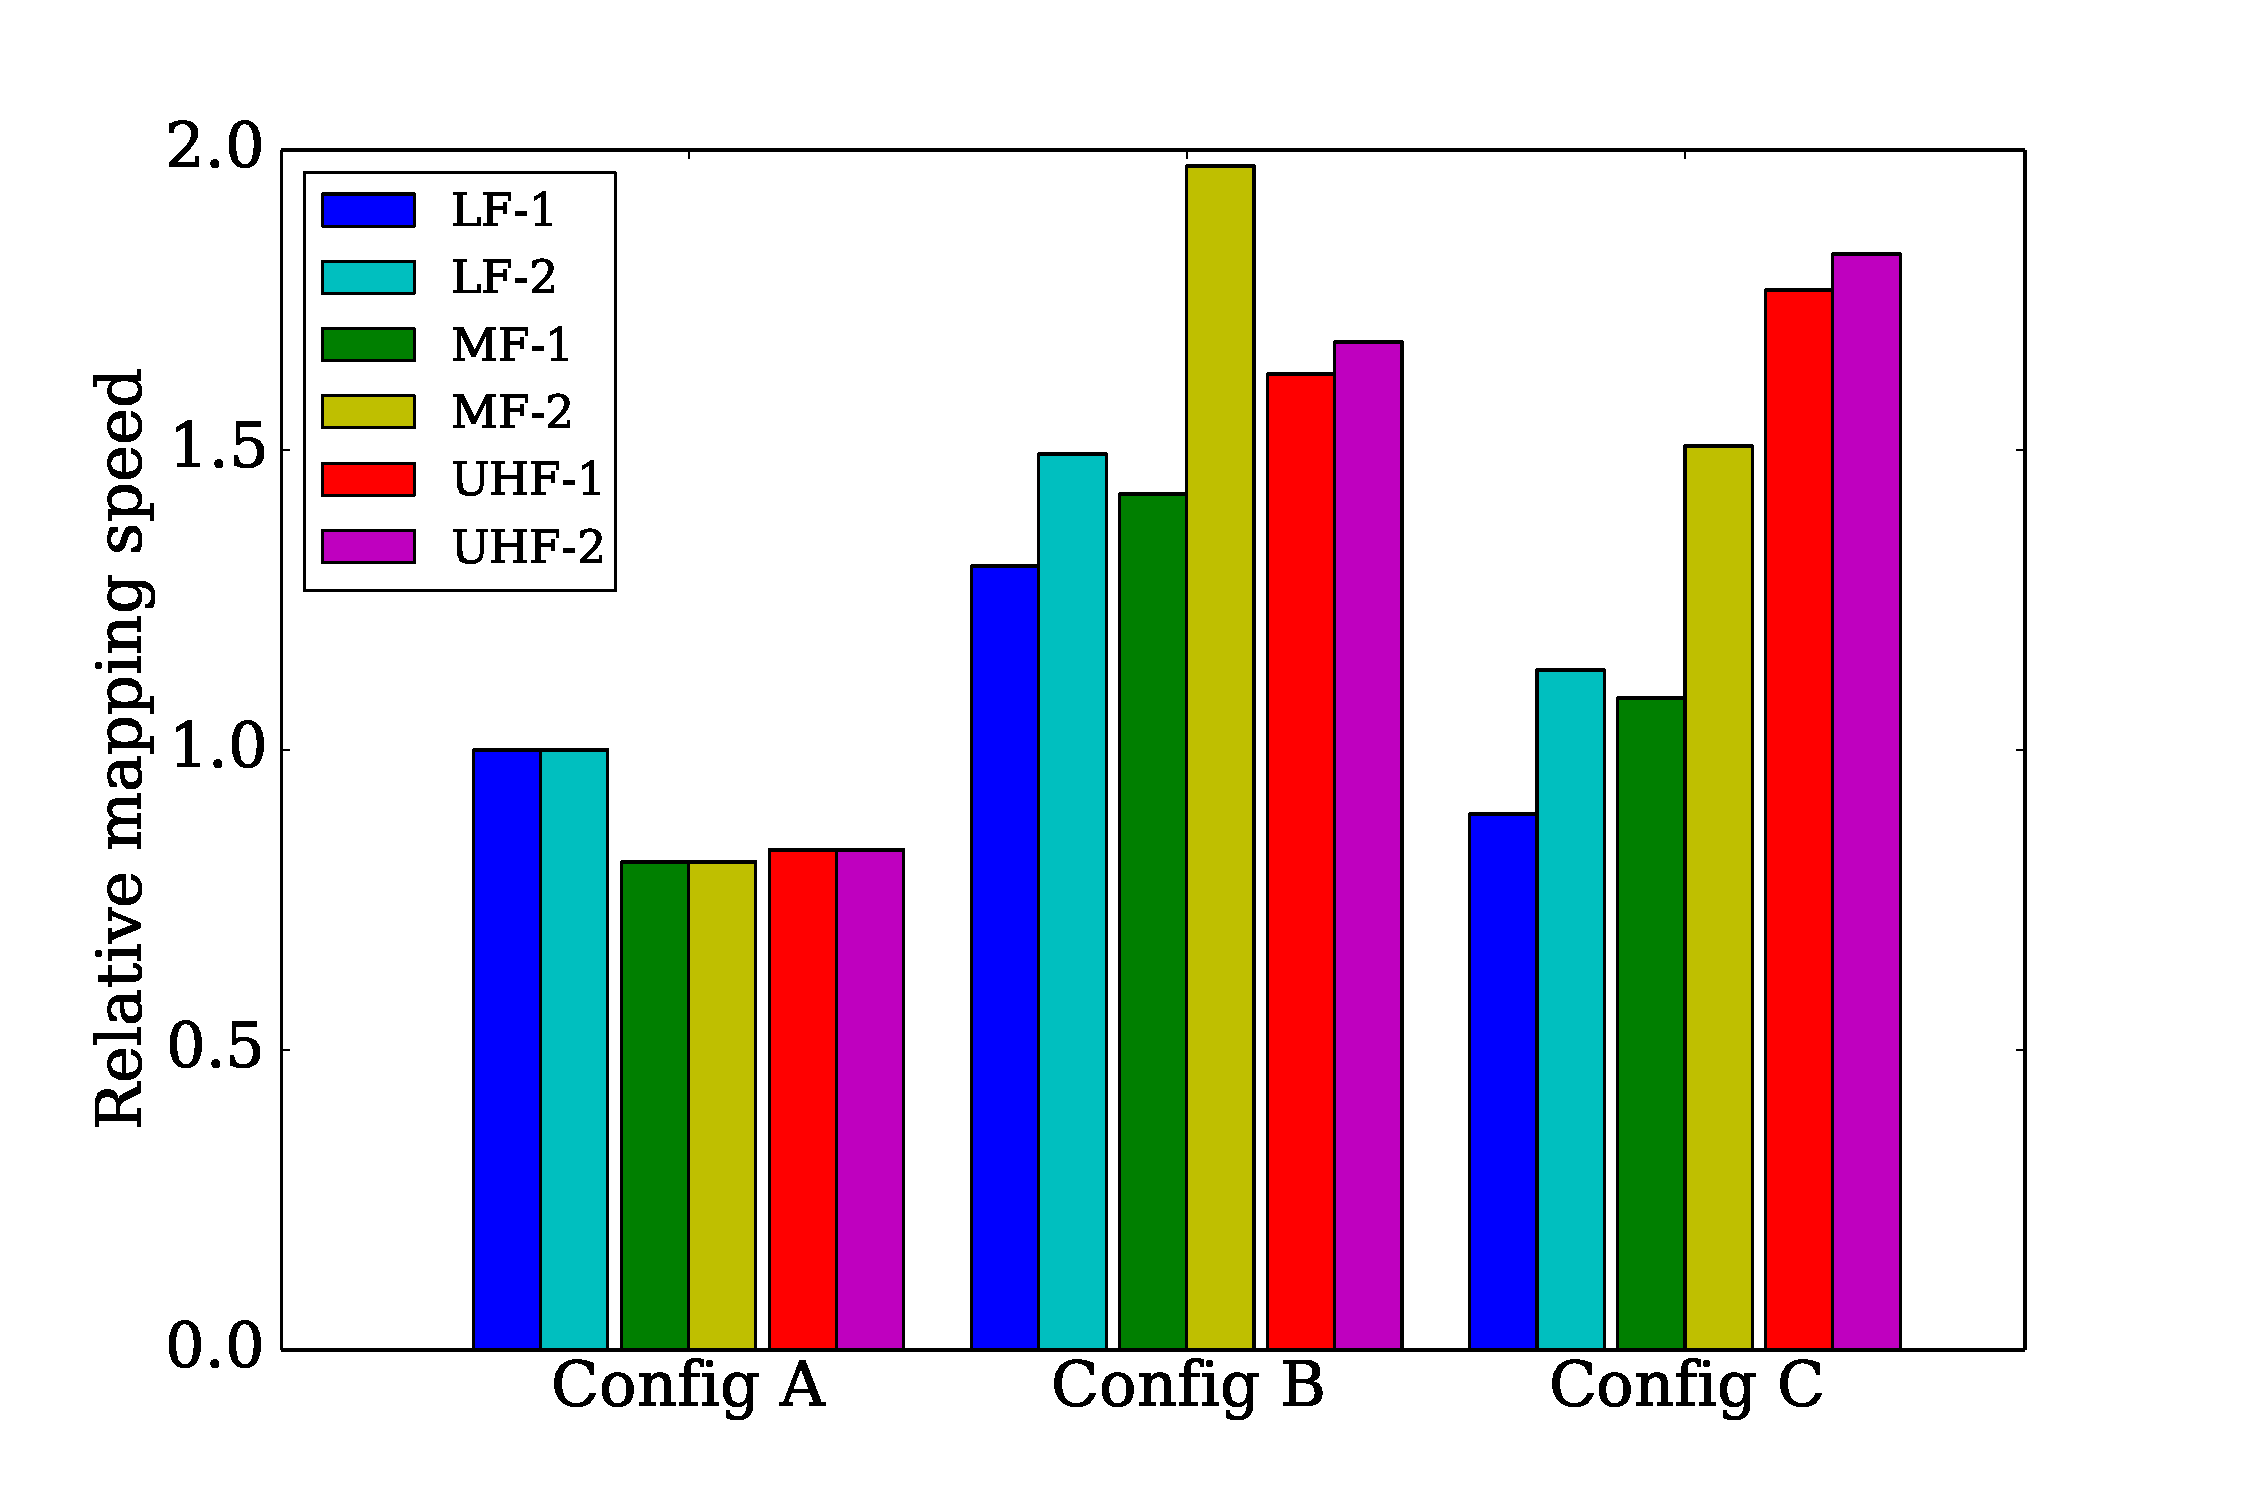
\includegraphics[width=0.58\linewidth, trim=1cm 1cm 2cm 2cm, clip]{BoloCalc/Figures/MSvsConfig.pdf}
    }
    \caption[Sensitivity comparison between candidate SO LAT configurations]{\ref{fig:so_ot_configs:a} shows three different camera packings that were investigated for the LAT. Config A has a maximum of 19~cameras with one~wafer per camera, Config B has 13~cameras with four~wafers per, and Config C has 7~cameras with seven~wafers per. Red circles represent UHF cameras, green MF, and blue LF. The outer-most black circle shows the maximum FOV offered by the telescope. Configs A and C do not fill the available telescope FOV due to limitations on the magnification and image quality of the cameras' reimaging optics. \ref{fig:so_ot_configs:b} shows the relative MS of each configuration for all six SO bands. Config B, when fully filled, is favored in all but the UHF bands.}
    \label{fig:so_ot_configs}
\end{figure}

%%%%%%%%%%%%%%%%%%%%%%%%%%%%%%%%
%%%%%%%%%%%%%%%%%%%%%%%%%%%%%%%%

\subsection{Camera magnification}
\label{sec:bolocalc_camera_magnification}

Another important application of BoloCalc within SO was to assess the impact of camera magnification on MS, which BoloCalc parameterizes using the F/\# at the focal plane. For a fixed FOV and pixel size, a smaller F/\# leads to higher spillover efficiency at the cold aperture stop and thus better sensitivity. However, if the F/\# is made too small, the Strehl ratio will begin to degrade at the edges of the focal plane, leading to fewer detectors with acceptable image quality. Therefore, it is useful to understand how rapidly MS varies with F/\# to inform the sensitivity impact of various reimaging optics designs. 

The degree to which a smaller F/\# improves MS depends on frequency and optical configuration. Figure~\ref{fig:bolocalc_so_fnum} shows the impact of F/\# on MS in both the LAT and the SAT given a fixed FOV and pixel size for the LF, MF, and UHF cameras. This calculation is combined with the results of ray-trace simulations to evaluate the performance of various camera optical designs.
%\cite{dicker_lat_2018}
The impact of F/\# on MS is most pronounced at low frequencies, where the spillover fraction and optical correlations tend to be largest. In contrast, the impact of F/\# on sensitivity is minimal at high frequencies where stop spillover and optical correlations tend to be small. Additionally, increasing per-detector throughput via a smaller F/\# most benefits the SAT, which does does not suffer from parasitic loading due to ambient-temperature mirrors. Section~\ref{sec:primspill} has more details on the impact of LAT warm spillover on MS.

\begin{figure}[!t]
	\subfloat[\label{fig:bolocalc_so_fnum:a}]{
    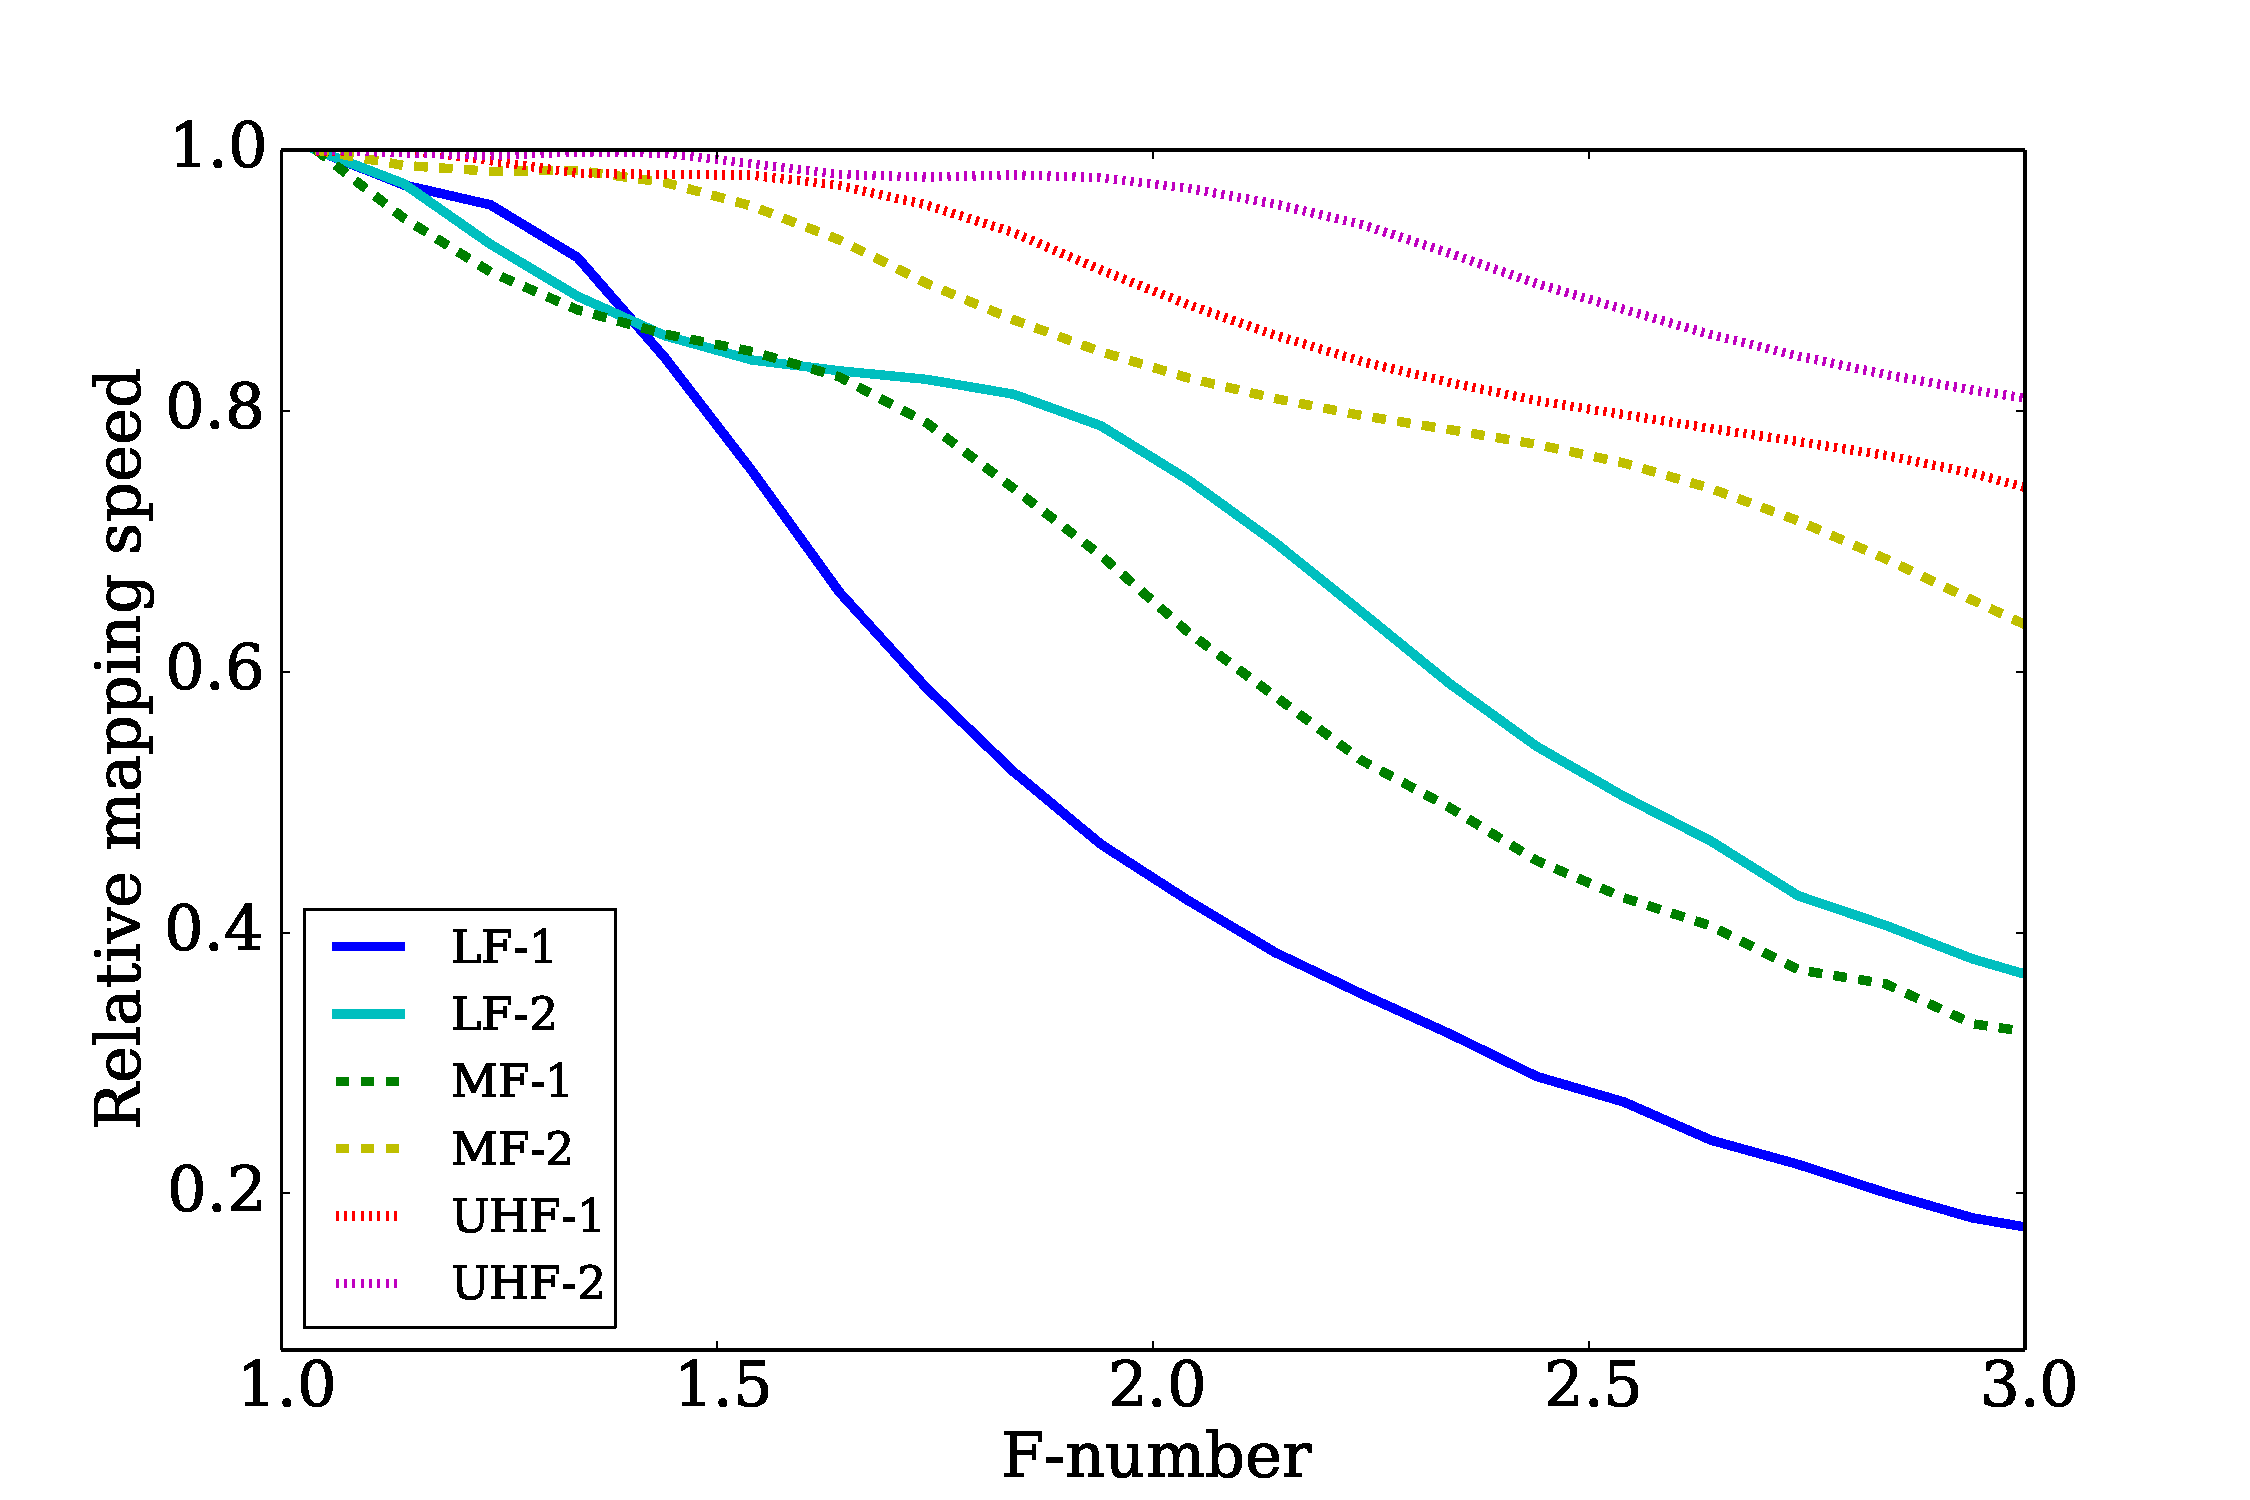
\includegraphics[trim={1.5cm, 0.2cm, 1.5cm, 1.5cm}, clip, width=0.48\linewidth]{BoloCalc/Figures/MSvsFnum_LAT.pdf}}
    \hfill
    \subfloat[\label{fig:bolocalc_so_fnum:b}]{
    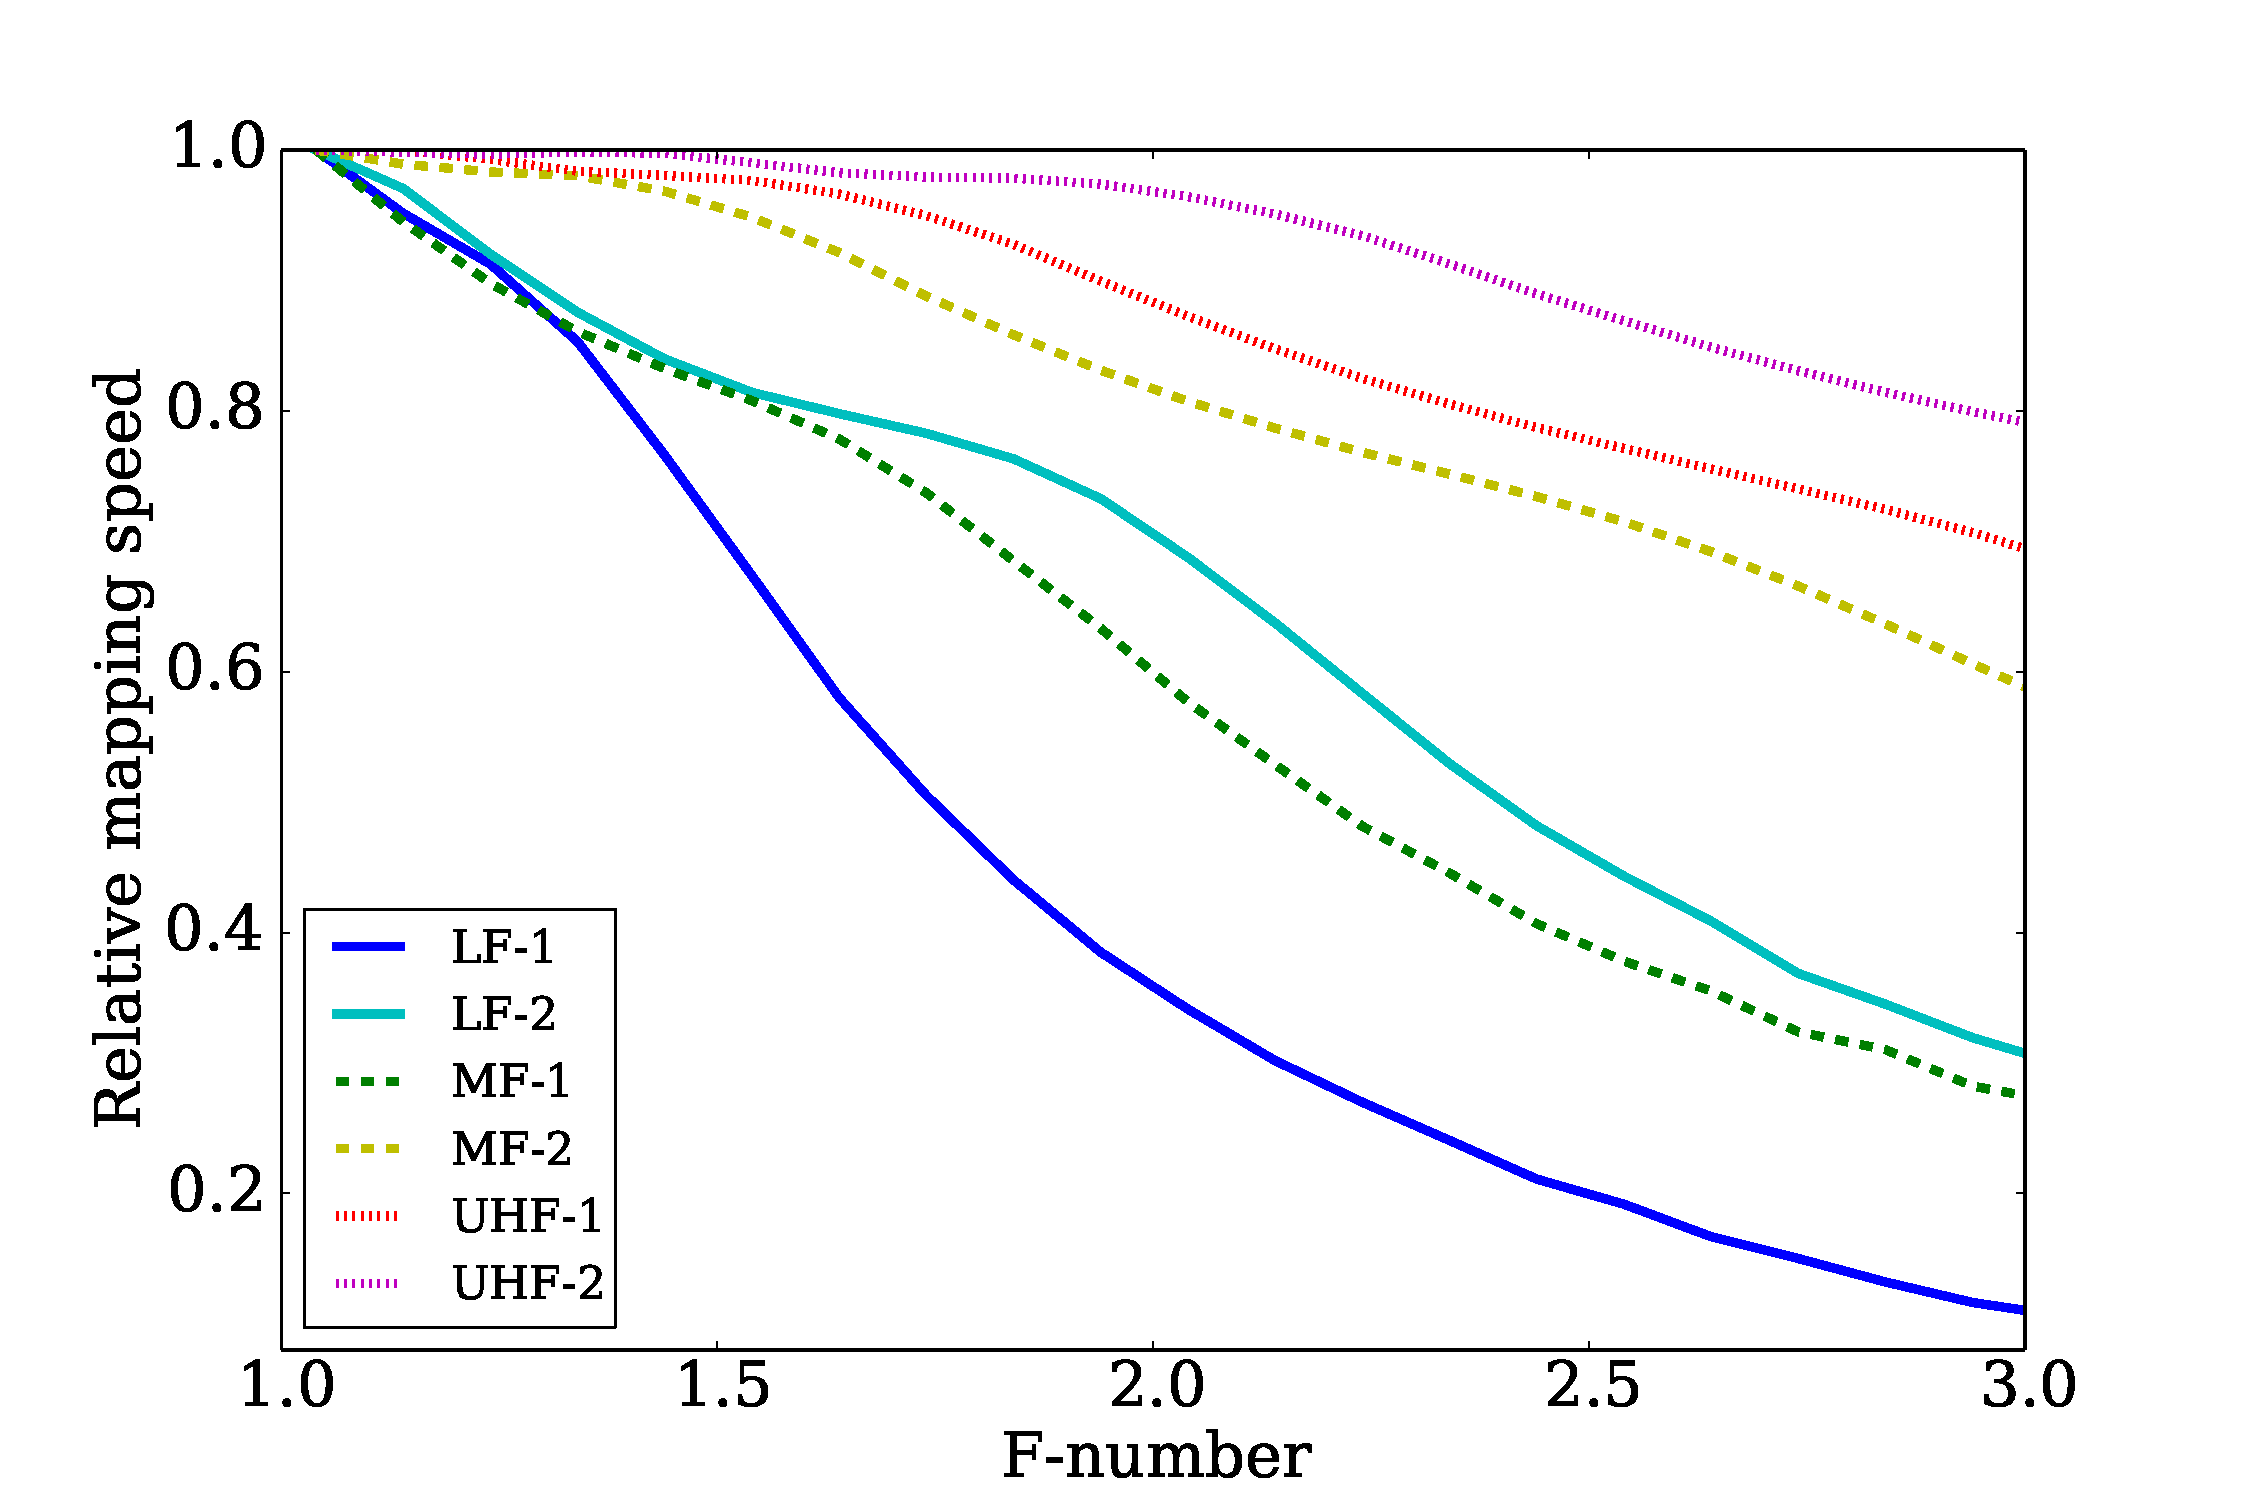
\includegraphics[trim={1.5cm, 0.2cm, 1.5cm, 1.5cm}, clip, width=0.48\linewidth]{BoloCalc/Figures/MSvsFnum_SAC.pdf}}
    \caption{Relative MS vs. camera F/\# in each frequency band in (a) the LAT and (b) the SAT. Given a fixed FOV and pixel size, smaller F/\# improves MS, but the impact is greater at lower frequency and in the SAT. The curves for each frequency channel are individually peak-normalized. \label{fig:bolocalc_so_fnum}}
\end{figure}

%%%%%%%%%%%%%%%%%%%%%%%%%%%%%%%%
%%%%%%%%%%%%%%%%%%%%%%%%%%%%%%%%

\subsection{Pixel pitch}
\label{sec:bolocalc_pixel_pitch}

Another important input to instrument design is the pixel pitch on the focal plane. As described in Section~\ref{sec:beam_coupling}, CMB detectors are single-moded and diffraction limited, so the aperture stop spillover efficiency can be approximated as a Gaussian function, parameterized by the ratio of the pixel pitch to the beam waist $w_{\mathrm{f}} = D / w_{\mathrm{0}}$
\begin{equation}
	\eta_{\mathrm{stop}} = 1 - \exp \Big[ -\frac{\pi^{2}}{2} \Big( \frac{D}{\lambda F w_{\mathrm{f}}} \Big)^{2} \Big]\, ,
    \label{eq:gauss}
\end{equation}
where $D$ is the pixel pitch (or equivalently, the pixel diameter), $F$ is the F/\# at the focal plane, and $\lambda$ is the observation wavelength. Smaller pixels have lower efficiency through the stop but allow for denser detector packing. Therefore, for a fixed FOV, there exists a pixel pitch for each frequency that maximizes MS. 

Figure~\ref{fig:so_pixel_pitch} shows MS vs. pixel pitch, plotted in units of $F \lambda$, for all SO frequencies in the LAT and SAT. In general, smaller pixels give higher MS, as the MS gain due to increased pixel density is faster than the MS degradation due to reduced stop spillover efficiency. The optimal $F \lambda$ spacing is largest in the LF camera as optical correlations are strongest at low frequencies where the photon occupation number is large. Additionally, the optimal $F \lambda$ pixel pitch in the LAT is smaller than that of the SAT, as the LAT has more parasitic ambient-temperature loading (see Section~\ref{sec:bolocalc_primary_spillover} for further discussion of LAT warm spillover). We also confirmed that the trends found from assuming Gaussian beams (Equation~\ref{eq:gauss}) were consistent with the integrated $\eta_{\mathrm{stop}}$ from full beam simulations for prototype feedhorn and lenslet designs at multiple pixel sizes.

There are many considerations when choosing pixel pitch, including systematic effects due to observing with electrically small antennas,
%\cite{crowley_so_2018}
diffraction artifacts from aggressive aperture truncation, %\cite{gallardo_lat_2018}
readout multiplexing factor,
%\cite{dober_microwave_2017}
wirebond density,
%\cite{ho_so_2018} 
achievable saturation power, 
%\cite{koopman_advanced_2018}
feedhorn and/or lenslet fabrication limitations,
%\cite{beckman_so_2018,simon_so_2018}
cost, etc. Going to smaller sizes is not always favorable when these extraneous considerations are taken into account, but understanding the MS differences between various focal plane layouts has been a critical input to the pixel pitch study.

\begin{figure}[!t]
	\subfloat[\label{fig:so_pixel_pitch:a}]{
    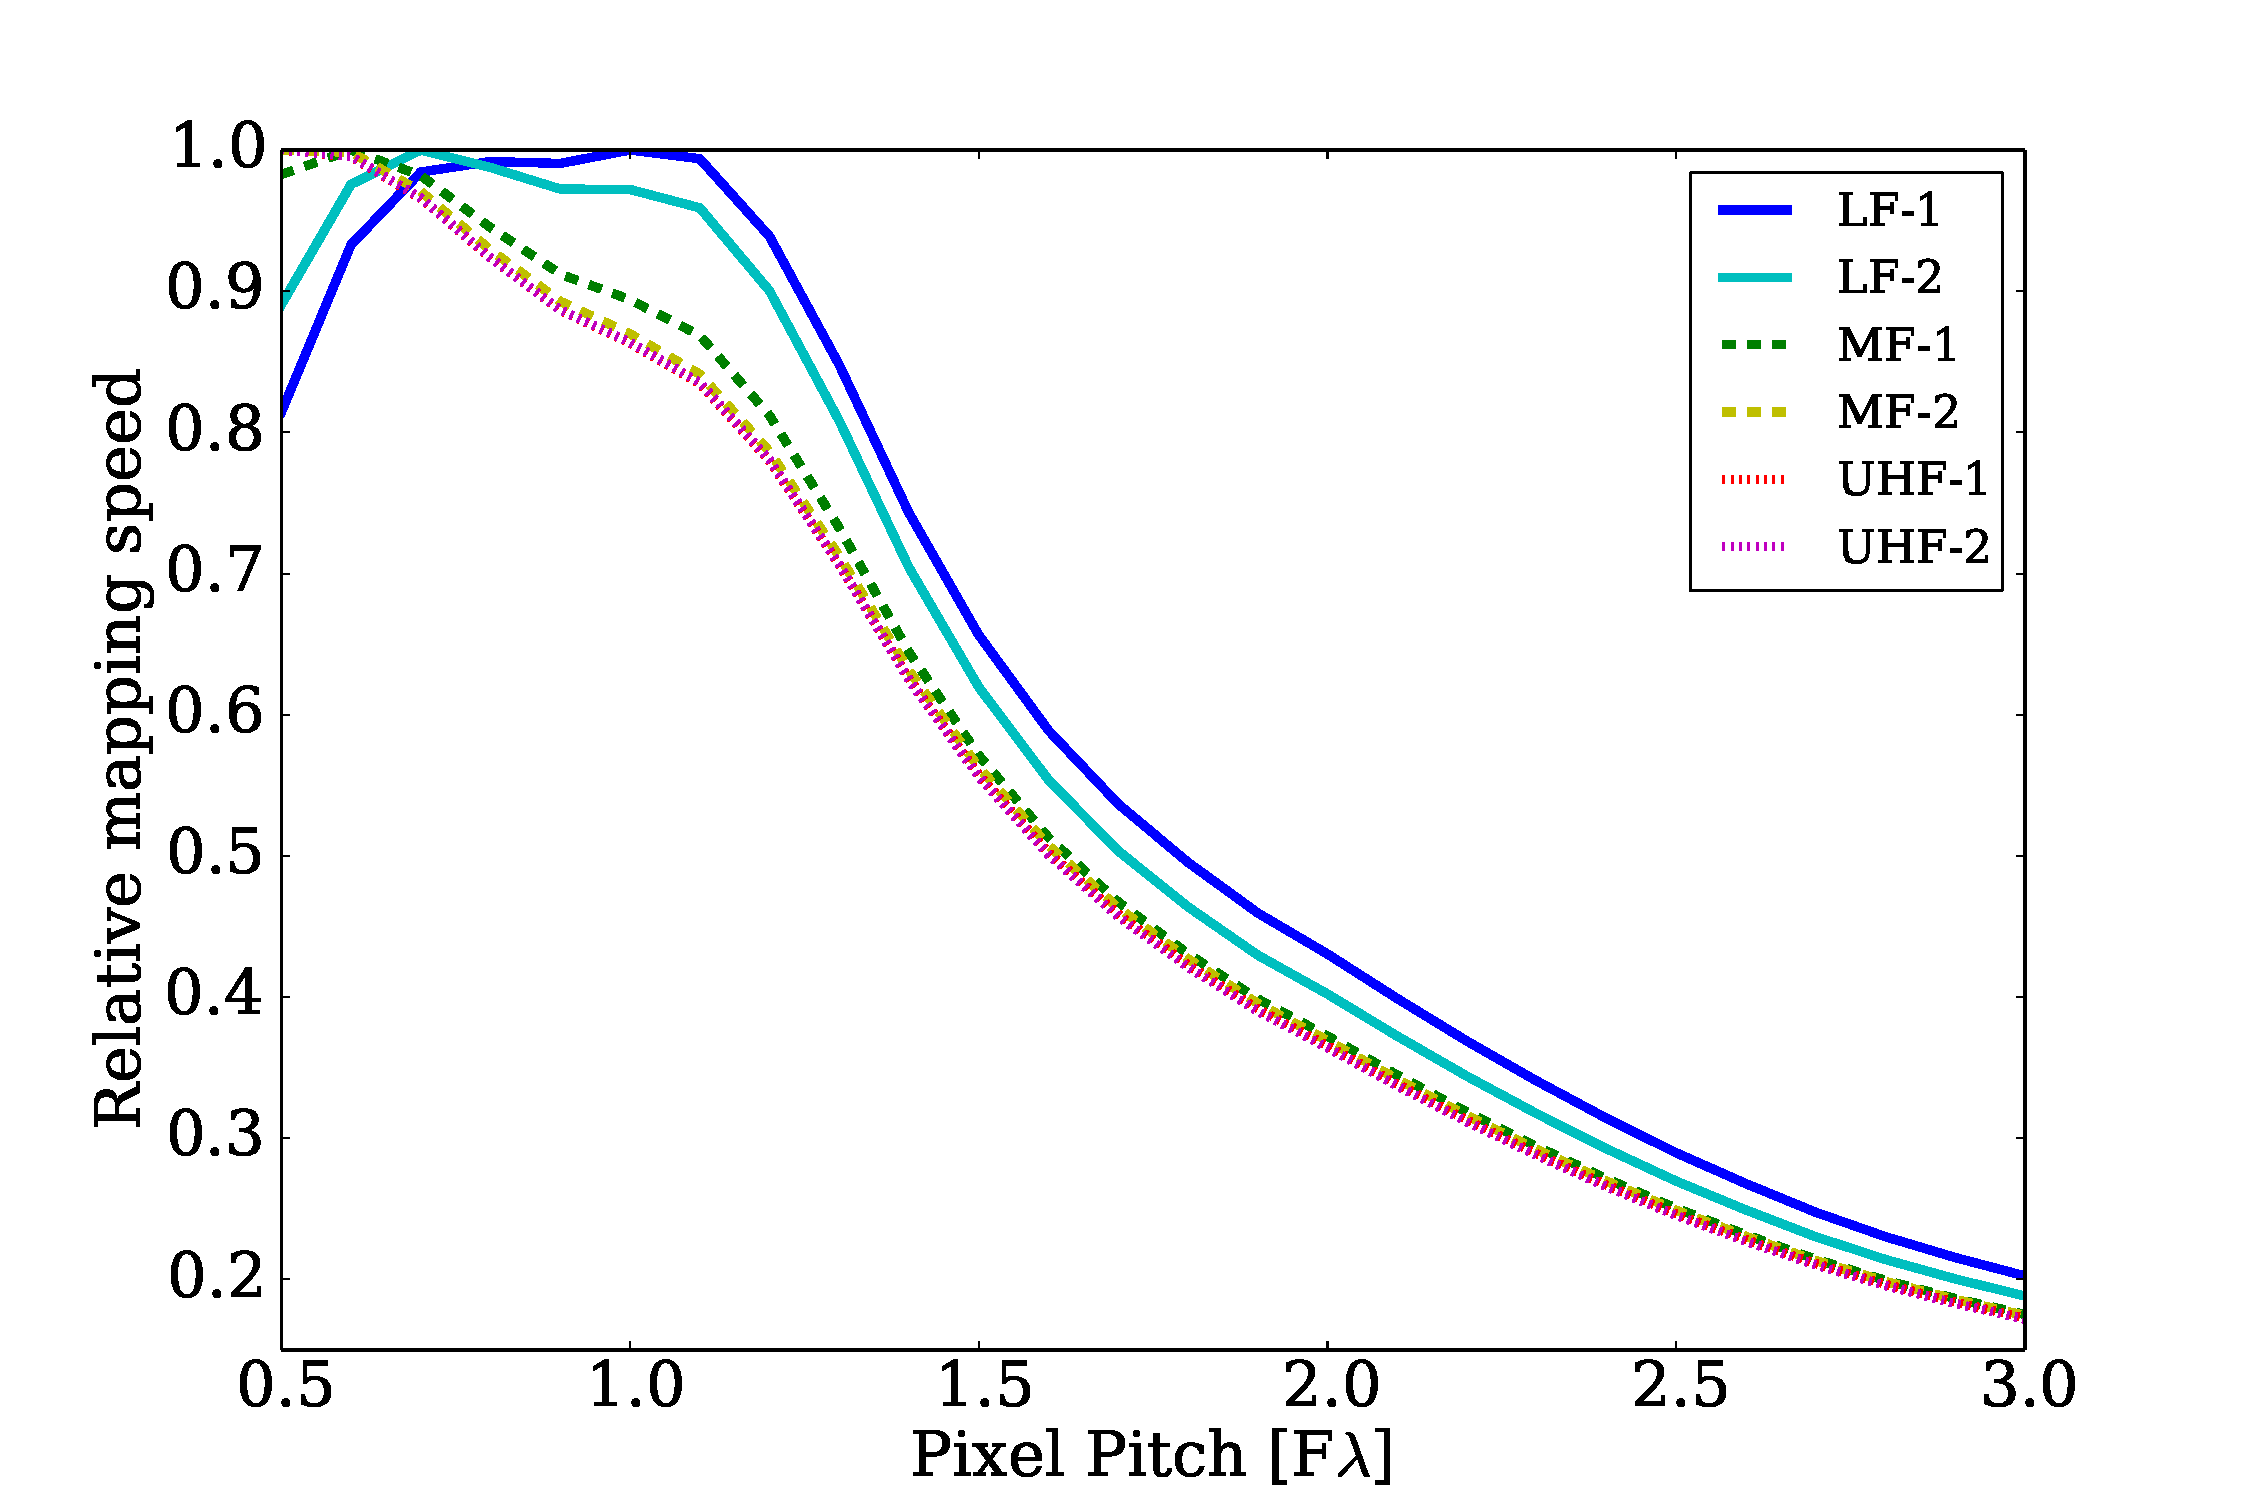
\includegraphics[trim={1.5cm, 0.2cm, 1.5cm, 1.5cm}, clip, width=0.48\linewidth]{BoloCalc/Figures/MSvsPixelSize_LAT.pdf}}
    \hfill
    \subfloat[\label{fig:so_pixel_pitch:b}]{
    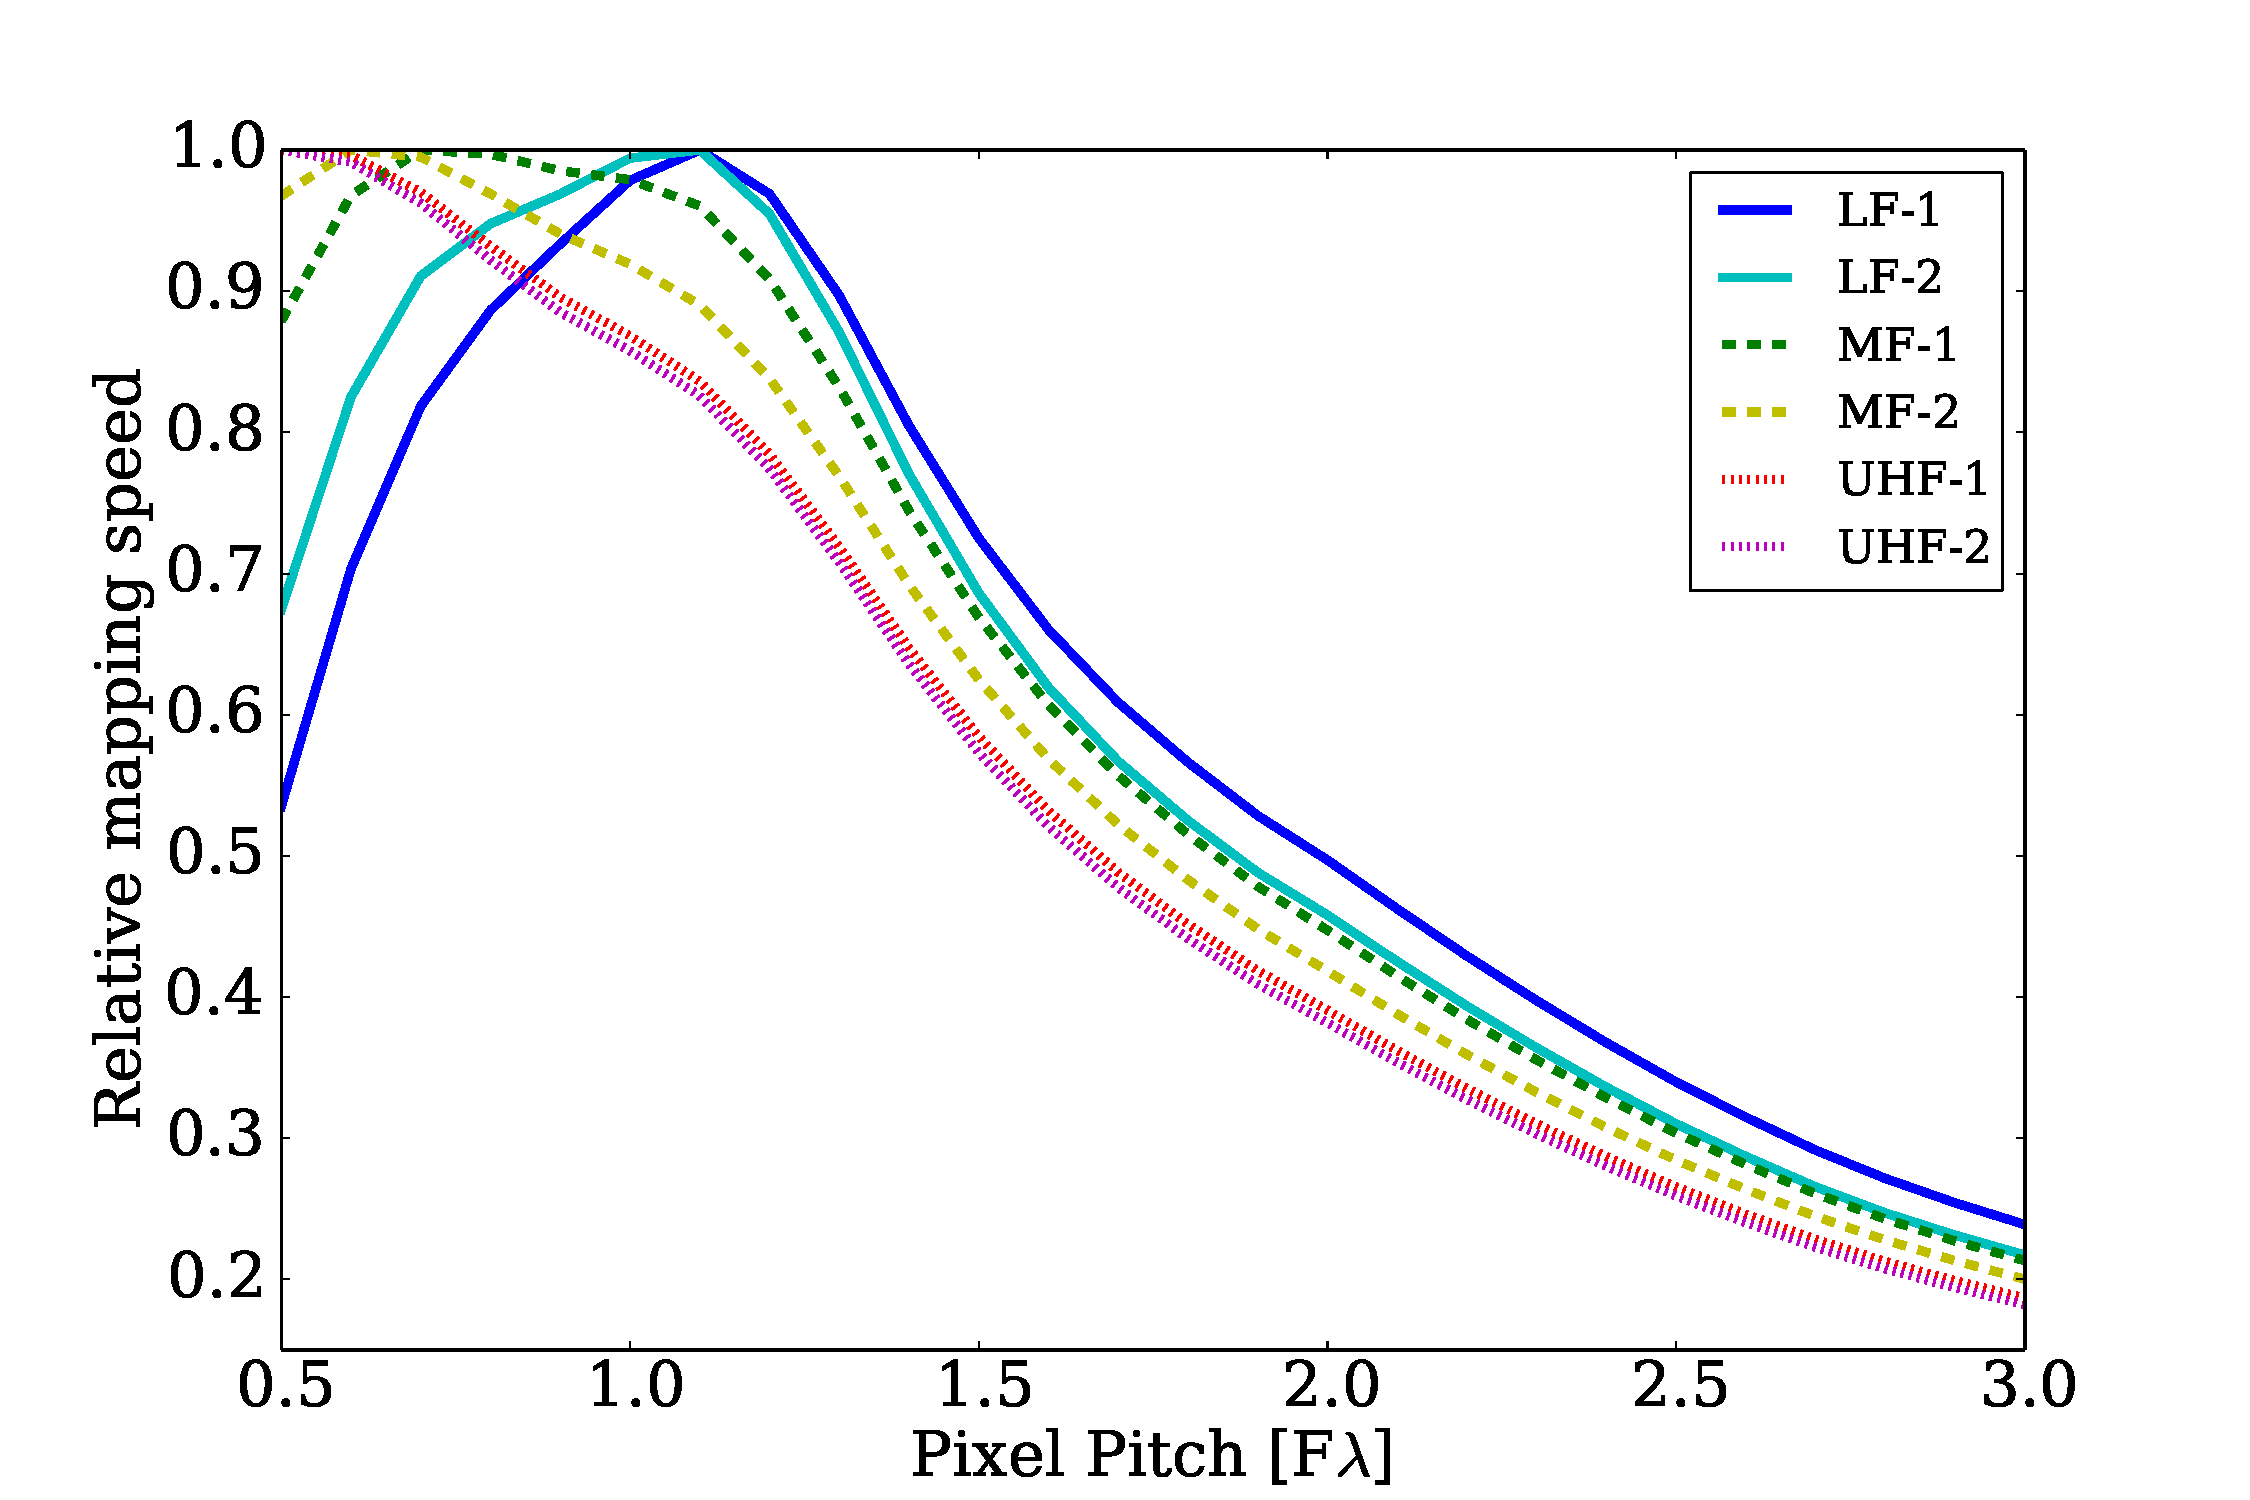
\includegraphics[trim={1.5cm, 0.2cm, 1.5cm, 1.5cm}, clip, width=0.48\linewidth]{BoloCalc/Figures/MSvsPixelSize_SAC.pdf}}
    \caption[Sensitivity comparison between candidate SO LAT configurations]{Relative MS in each frequency band in (a) the LAT and (b) the SAT against pixel pitch, plotted in units of $F \lambda$. Smaller pixels are favored until pitches $\sim$ 1.2~$F \lambda$, at which point the MS curve flattens due to detector-to-detector optical correlations. The curves for each frequency channel are individually peak-normalized.}
    \label{fig:so_pixel_pitch}
\end{figure}

%%%%%%%%%%%%%%%%%%%%%%%%%%%%%%%%
%%%%%%%%%%%%%%%%%%%%%%%%%%%%%%%%

\subsection{LAT primary spillover}
\label{sec:bolocalc_primary_spillover}

The LAT has a 6~m-diameter primary mirror, a 7.8~degree FOV, and up to 13~cameras in a 2.4~m diameter receiver that cover more than a decade in frequency 
%\cite{galitzki_so_2018,orlowski-sherer_latr_2018,dicker_lat_2018}.
Motivated by the immensity and complexity of the LAT system, effort has been devoted to understanding and controlling ambient-temperature spillover and scattering, 
%\cite{gallardo_lat_2018}
as minimizing optical loading is critical to maintaining low $\mathrm{NEP}_{\mathrm{ph}}$. 

Figure~\ref{fig:MSvsSpill} shows relative in-band optical power and MS in each frequency band as a function of LAT primary spillover fraction. The impact of primary spillover on both optical power and MS is largest at low frequencies, where loading due to other sources---such as atmospheric emission and camera thermal emission---is low and the optical efficiency---determined by the absorptivity of the lenses, filters, and on-chip transmission lines---is high. Additionally, the impact of primary spillover on MS is steep, making LAT optical simulations and baffling design a top priority within SO.

\begin{figure}[!t]
    \subfloat[\label{fig:so_primary_spillover:a}]{
    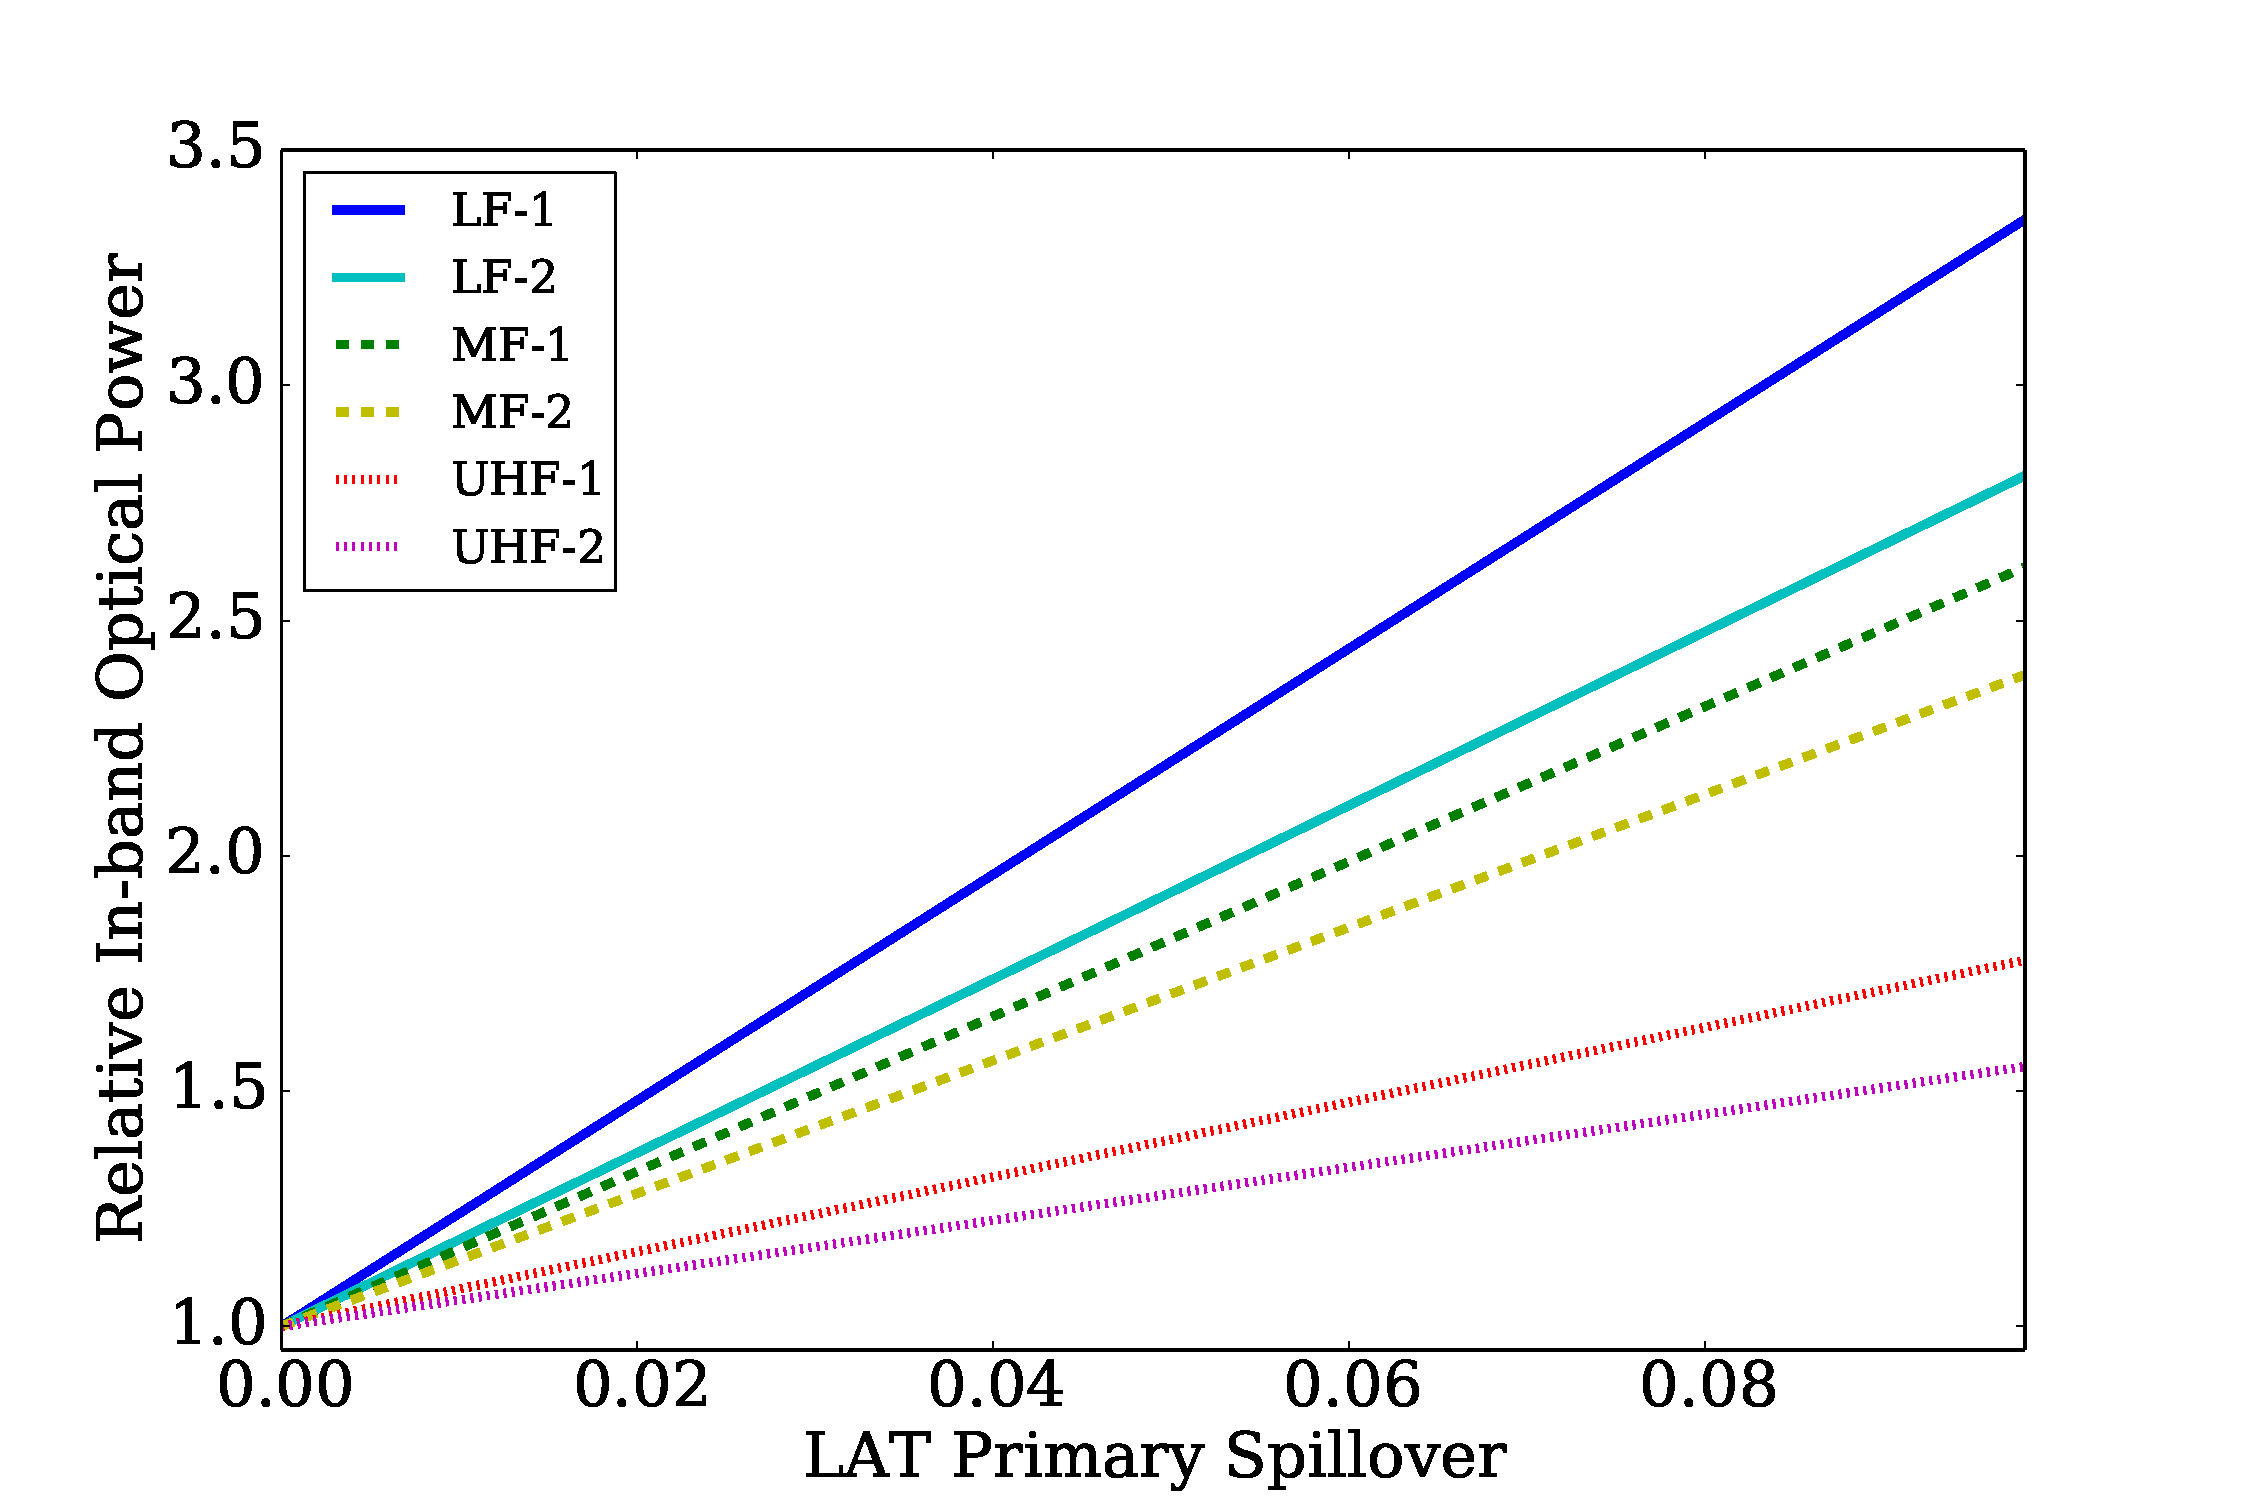
\includegraphics[trim={1.5cm, 0.1cm, 1.5cm, 1.5cm}, clip, width=0.48\linewidth]{BoloCalc/Figures/POvsPrimSpill_LAT.pdf}}
    \hfill
    \subfloat[\label{fig:so_primary_spillover:b}]{
    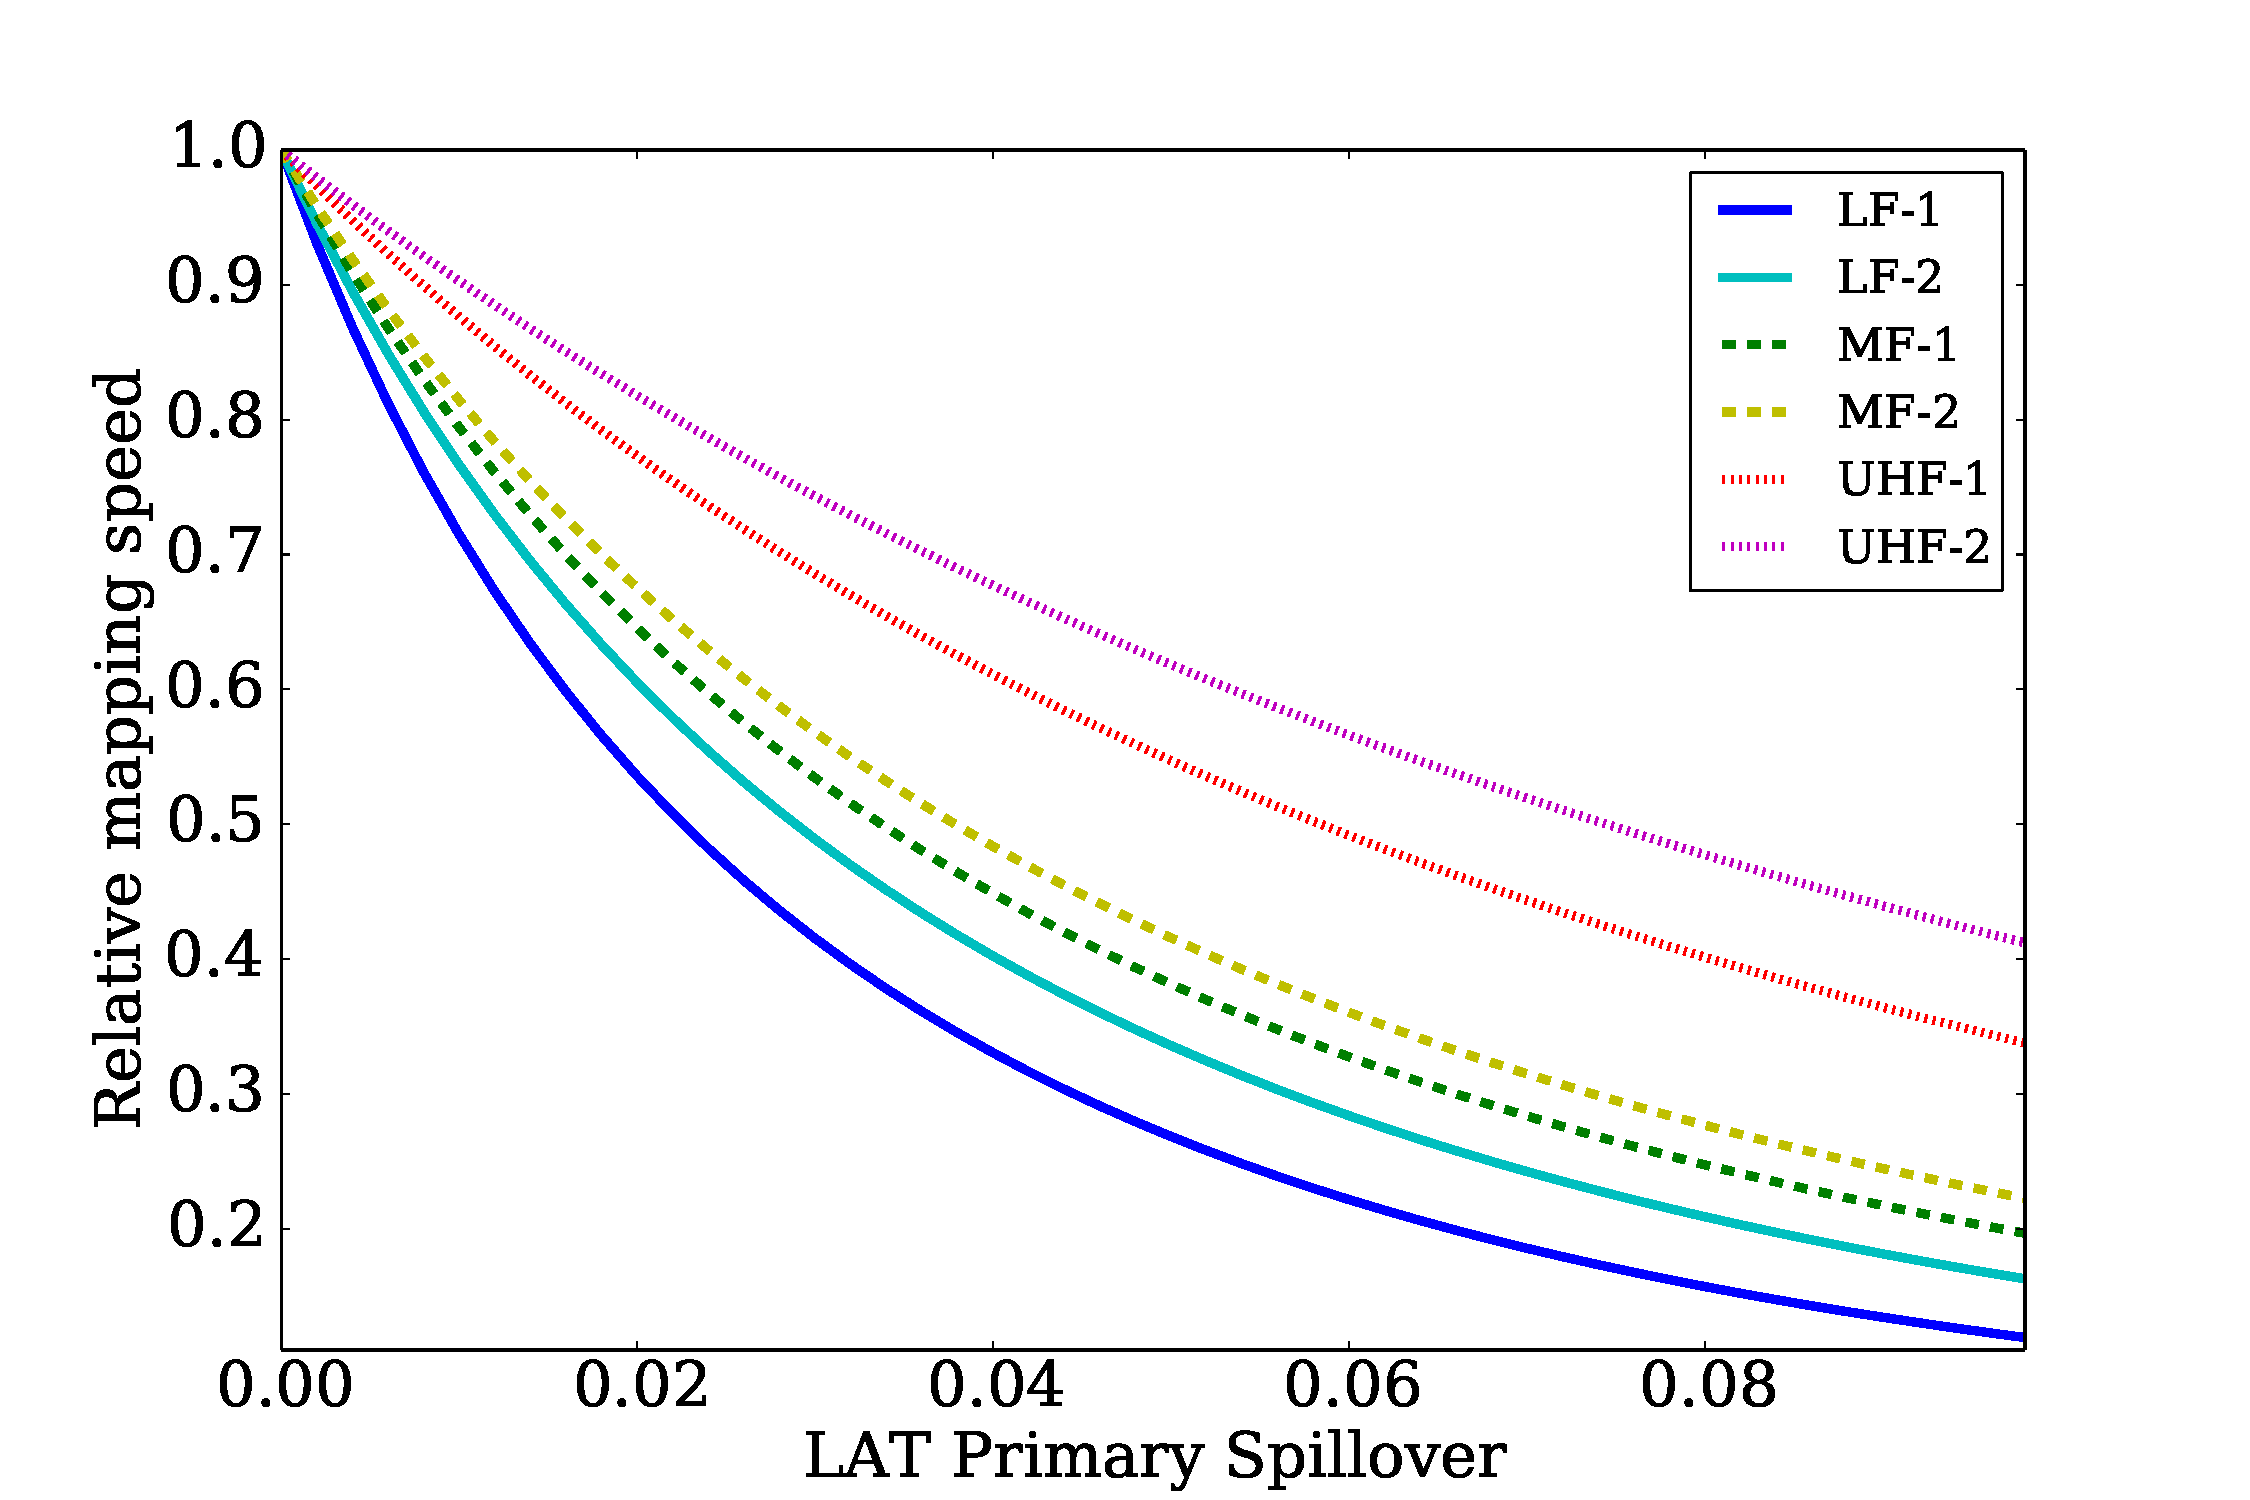
\includegraphics[trim={1.5cm, 0.1cm, 1.5cm, 1.5cm}, clip, width=0.48\linewidth]{BoloCalc/Figures/MSvsPrimSpill_LAT.pdf}}
    \caption[Impact of SO LAT primary spillover on optical power and mapping speed]{The relative optical power (a) and MS (b) in each LAT frequency band vs. primary spillover fraction. Lower spillover is always better for sensitivity, but the MS impact is more pronounced at low frequencies. The curves for each frequency channel are individually peak-normalized.}
    \label{fig:so_primary_spillover}
\end{figure}

%%%%%%%%%%%%%%%%%%%%%%%%%%%%%%%%
%%%%%%%%%%%%%%%%%%%%%%%%%%%%%%%%

\subsection{SAT aperture stop temperature}
\label{sec:bolocalc_sat_stop_temperature}

Because the SAT does not suffer from loading due to ambient-temperature mirrors, the most important contribution to $\mathrm{NEP}_{\mathrm{ph}}$ is the temperature of the aperture stop. Therefore, understanding how stop temperature impacts MS is critical to setting its cooling requirement. 
%\cite{galitzki_so_2018}
The SAT stop is cooled by the 1~K stage of the dilution refrigerator and is connected to that stage via a long heat strap. Sky-side IR is filtered out by a combination of IR shaders, reflective low-pass filters, and alumina absorbing filters. A calculation of NET vs stop temperature was used to inform the telescope's thermal design and heat strapping infrastructure.

Figure~\ref{fig:so_stop_temperature} shows relative in-band optical power and MS as a function of stop temperature for all the SAT frequency bands. The impact of stop temperature is largest at low frequencies where other sources of parasitic loading---such as atmosphere and lens emission---are small. Additionally, its impact is more dramatic in the low band of each dichroic pixel, as that channel has a lower stop spillover efficiency due a smaller $D / F \lambda$ pixel size (see Equation~\ref{eq:gauss}). Finally, its impact at high frequencies is negligible because the SAT UHF pixels are electrically large and therefore spill little power onto the stop. 

\begin{figure}[!t]
    \subfloat[\label{fig:so_stop_temperature:a}]{
    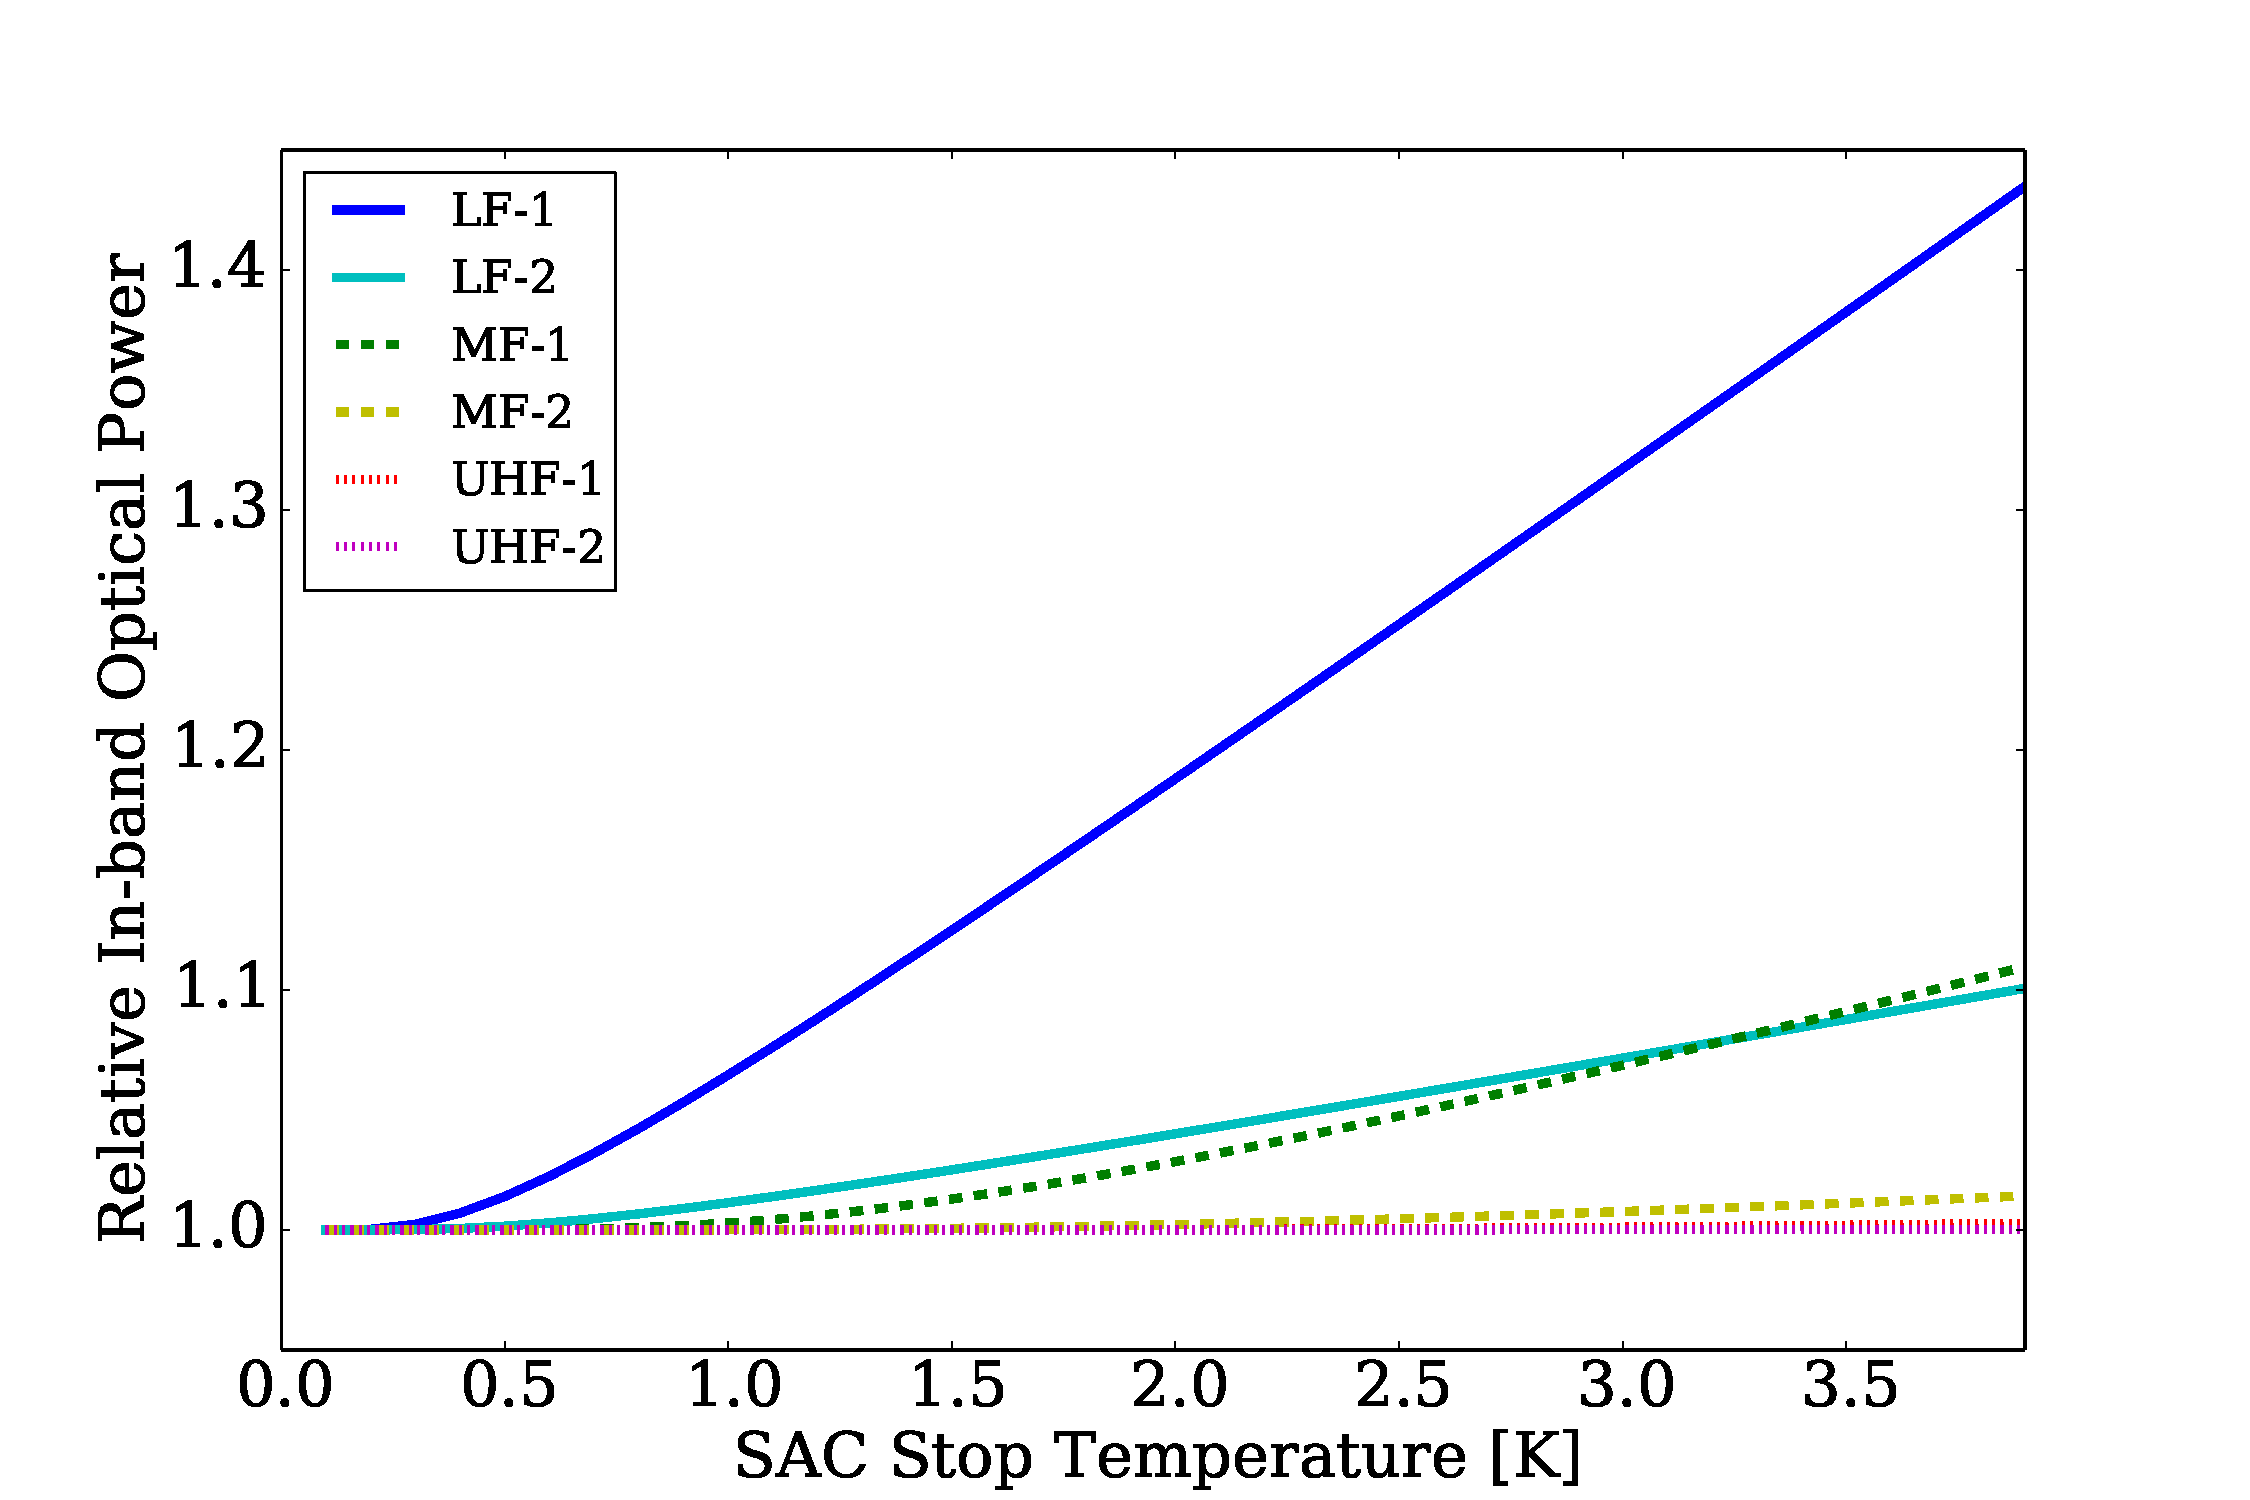
\includegraphics[trim={1.0cm, 0.1cm, 1.5cm, 1.5cm}, clip, width=0.48\linewidth]{BoloCalc/Figures/POvsStopTemp_SAC.pdf}}
    \hfill
    \subfloat[\label{fig:so_stop_temperature:b}]{
    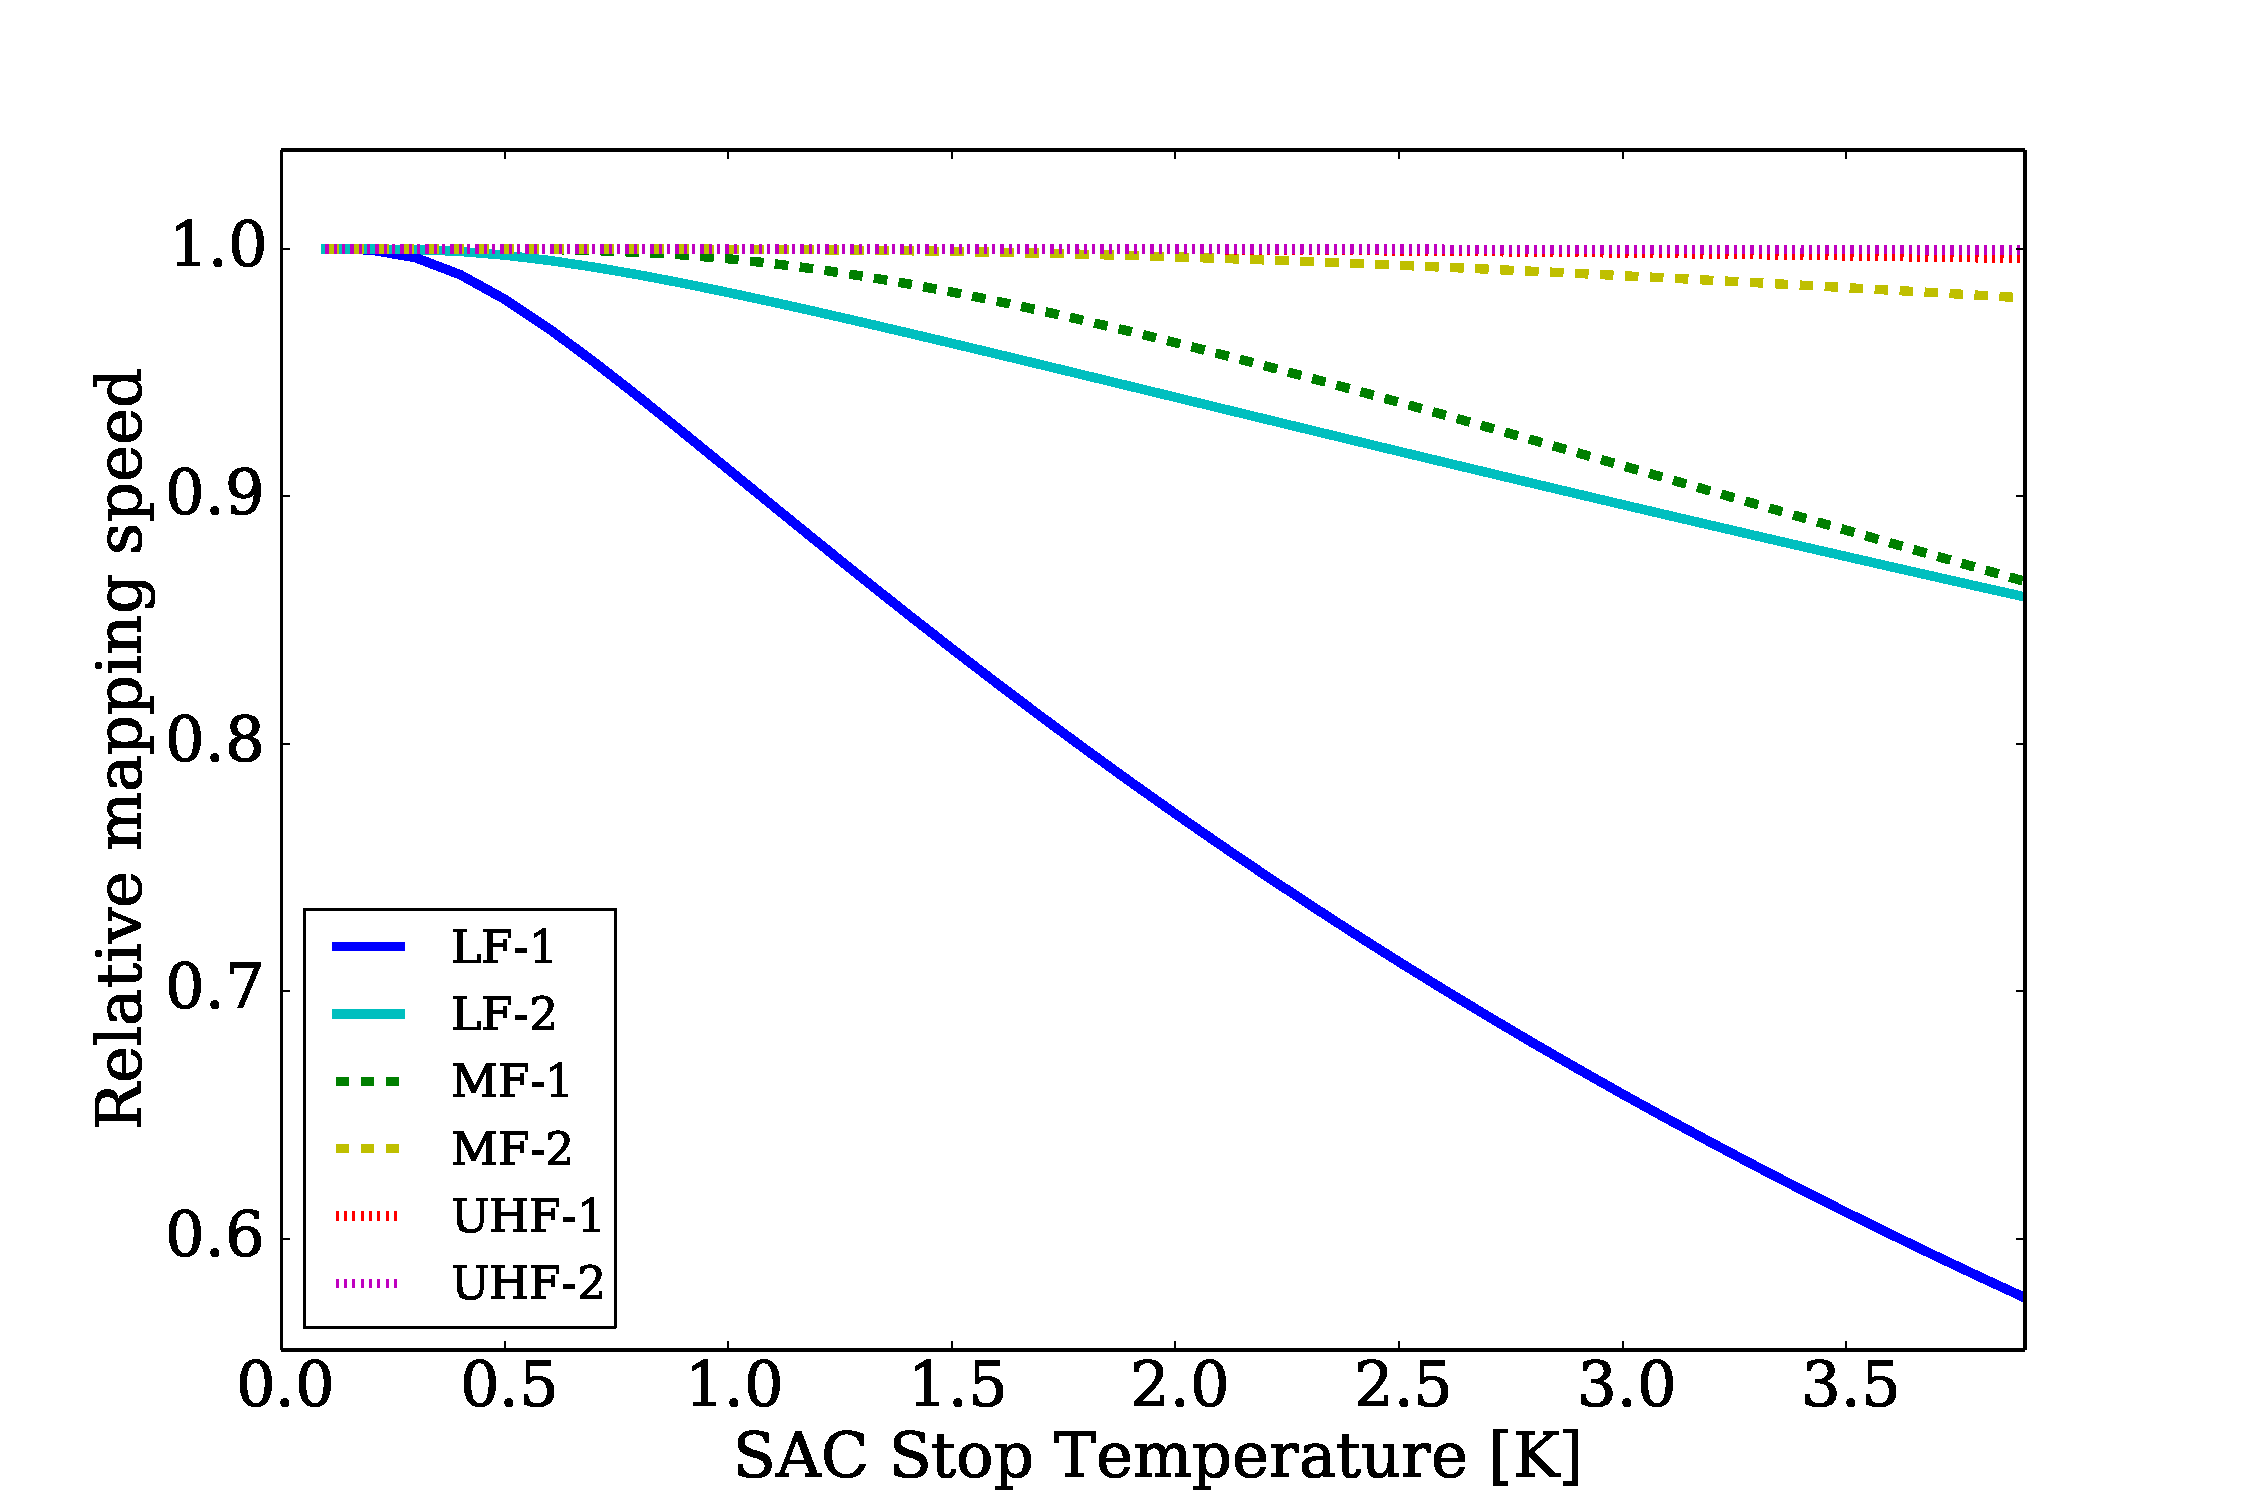
\includegraphics[trim={1.0cm, 0.1cm, 1.5cm, 1.5cm}, clip, width=0.48\linewidth]{BoloCalc/Figures/MSvsStopTemp_SAC.pdf}}
    \caption{Relative optical power (a) and MS (b) in each frequency band vs. SAT aperture stop temperature. Lower stop temperature is always better for sensitivity, but the impact tends to be larger at low frequencies, where other sources of parasitic loading are small, and in the low band of each dichroic pixel, where the pixel antenna beams are largest. The curves for each frequency channel are individually peak-normalized. \label{fig:so_stop_temperature}}
\end{figure}

%%%%%%%%%%%%%%%%%%%%%%%%%%%%%%%%
%%%%%%%%%%%%%%%%%%%%%%%%%%%%%%%%

\subsection{Detector saturation power}
\label{sec:bolocalc_so_psat_optimization}

In addition to characterizing sources of optical loading, BoloCalc can also be used to investigate the impact of detector parameters on sensitivity, including operation temperature, thermal conductivity to the bath, and on-chip optical efficiency. Such calculations can be used to set tolerances on fabrication targets and provide evaluation criteria for detector testing and quality control. Figure~\ref{fig:so_psat} shows relative MS vs. bolometer saturation power $P_{\mathrm{sat}}$, plotted as a fraction of optical power $P_{\mathrm{opt}}$, for both the LAT and SAT in each frequency band. The lowest possible value for $P_{\mathrm{sat}} / P_{\mathrm{opt}}$ is $1$, which corresponds to zero voltage bias across the bolometer, and the typical range of values that ensure linear bolometer operation is 2--3. 

Selecting a $P_{\mathrm{sat}}$ depends on several considerations including detector linearity, 
%\cite{crowley_so_2018}
stability of observing conditions,
%\cite{stevens_so_2018} 
and uncertainty in expected optical loading, but lower saturation power is always better for sensitivity. The impact of $P_{\mathrm{sat}} / P_{\mathrm{opt}}$ is largest in the LF bands where $\mathrm{NEP}_{\mathrm{ph}}$ is smallest and hence where $\mathrm{NEP}_{\mathrm{g}}$ makes the largest contribution to the total NET. The impact of $P_{\mathrm{sat}} / P_{\mathrm{opt}}$ is similar in the LAT and SAT because $\sqrt{P_{\mathrm{sat}} / P_{\mathrm{opt}}} \appropto \mathrm{NEP}_{\mathrm{g}} / \mathrm{NEP}_{\mathrm{ph}}$ (see Equations~\ref{eq:nep_ph} and~\ref{eq:nep_g}), modulated only by wave noise, which is similar in both telescopes. 

As SO has matured, BoloCalc has continued to play a key role in connecting detector and optical design, as an accurate calculation of optical power on the bolometer is important to setting its target parameters. Additionally, as SO detectors begin to undergo evaluation and as the uncertainty in expected optical loading decreases, BoloCalc is increasingly useful for tuning detector performance to maximize MS.

\begin{figure}[!t]
	\subfloat[\label{fig:so_psat:a}]{
    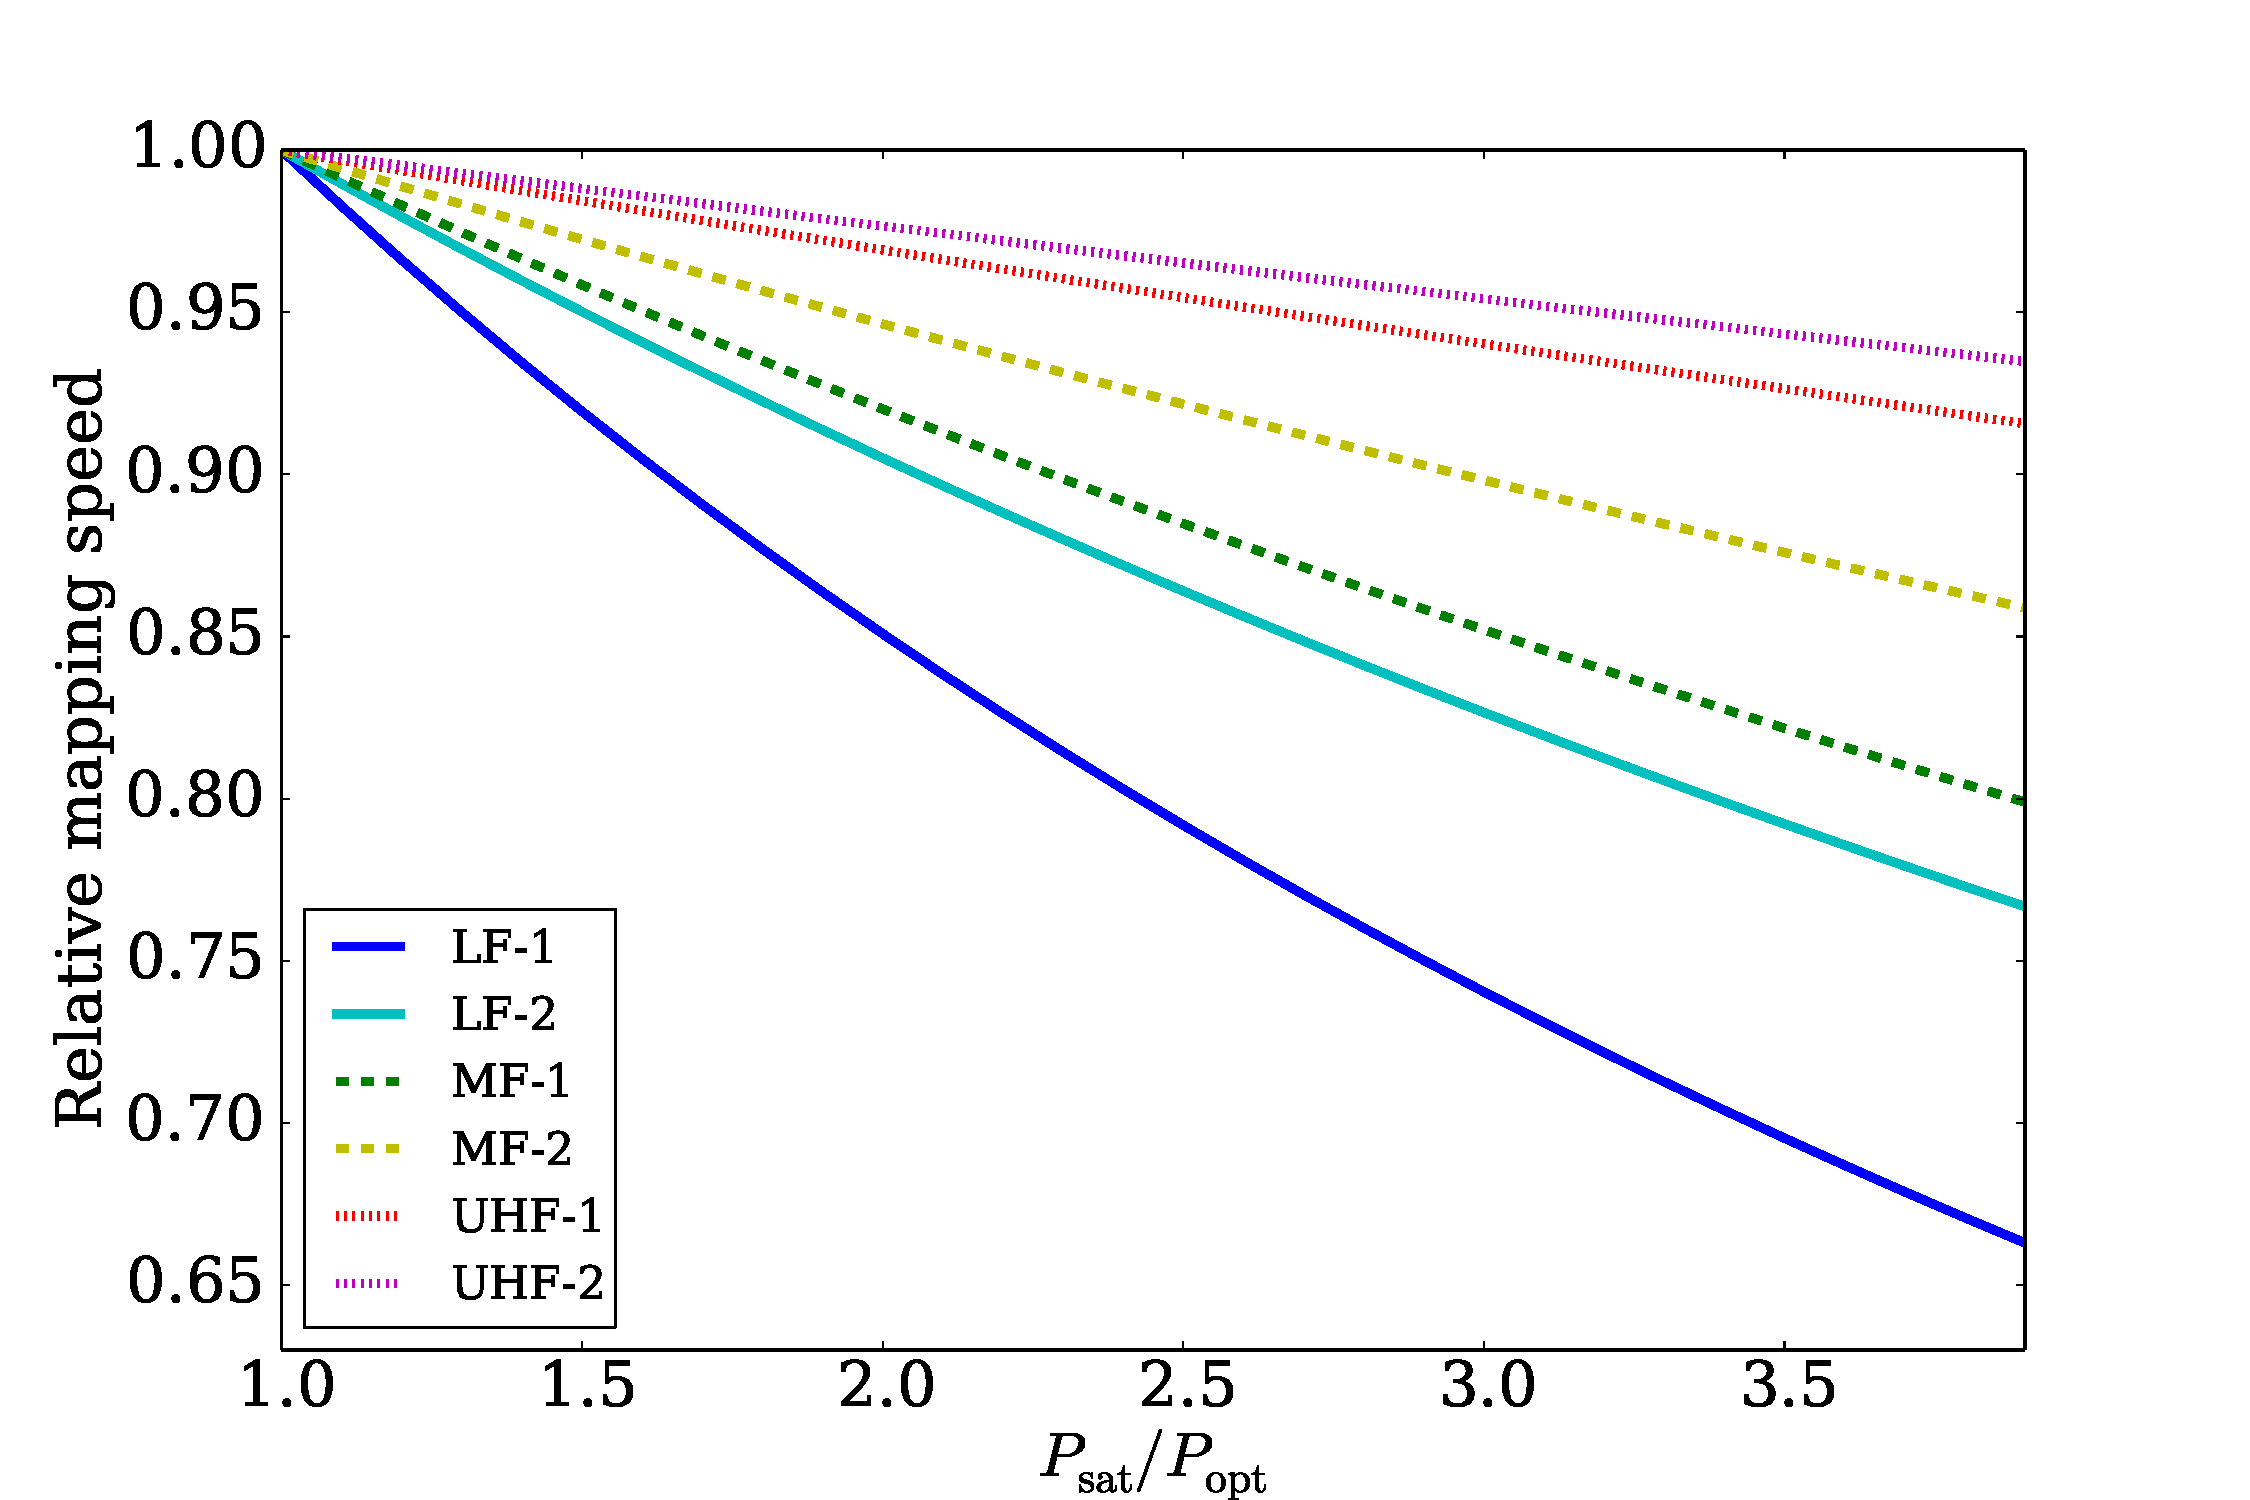
\includegraphics[trim={0.8cm, 0.0cm, 1.5cm, 1.5cm}, clip, width=0.48\linewidth]{BoloCalc/Figures/MSvsPsat_LAT.pdf}}
    \hfill
    \subfloat[\label{fig:so_psat:b}]{
    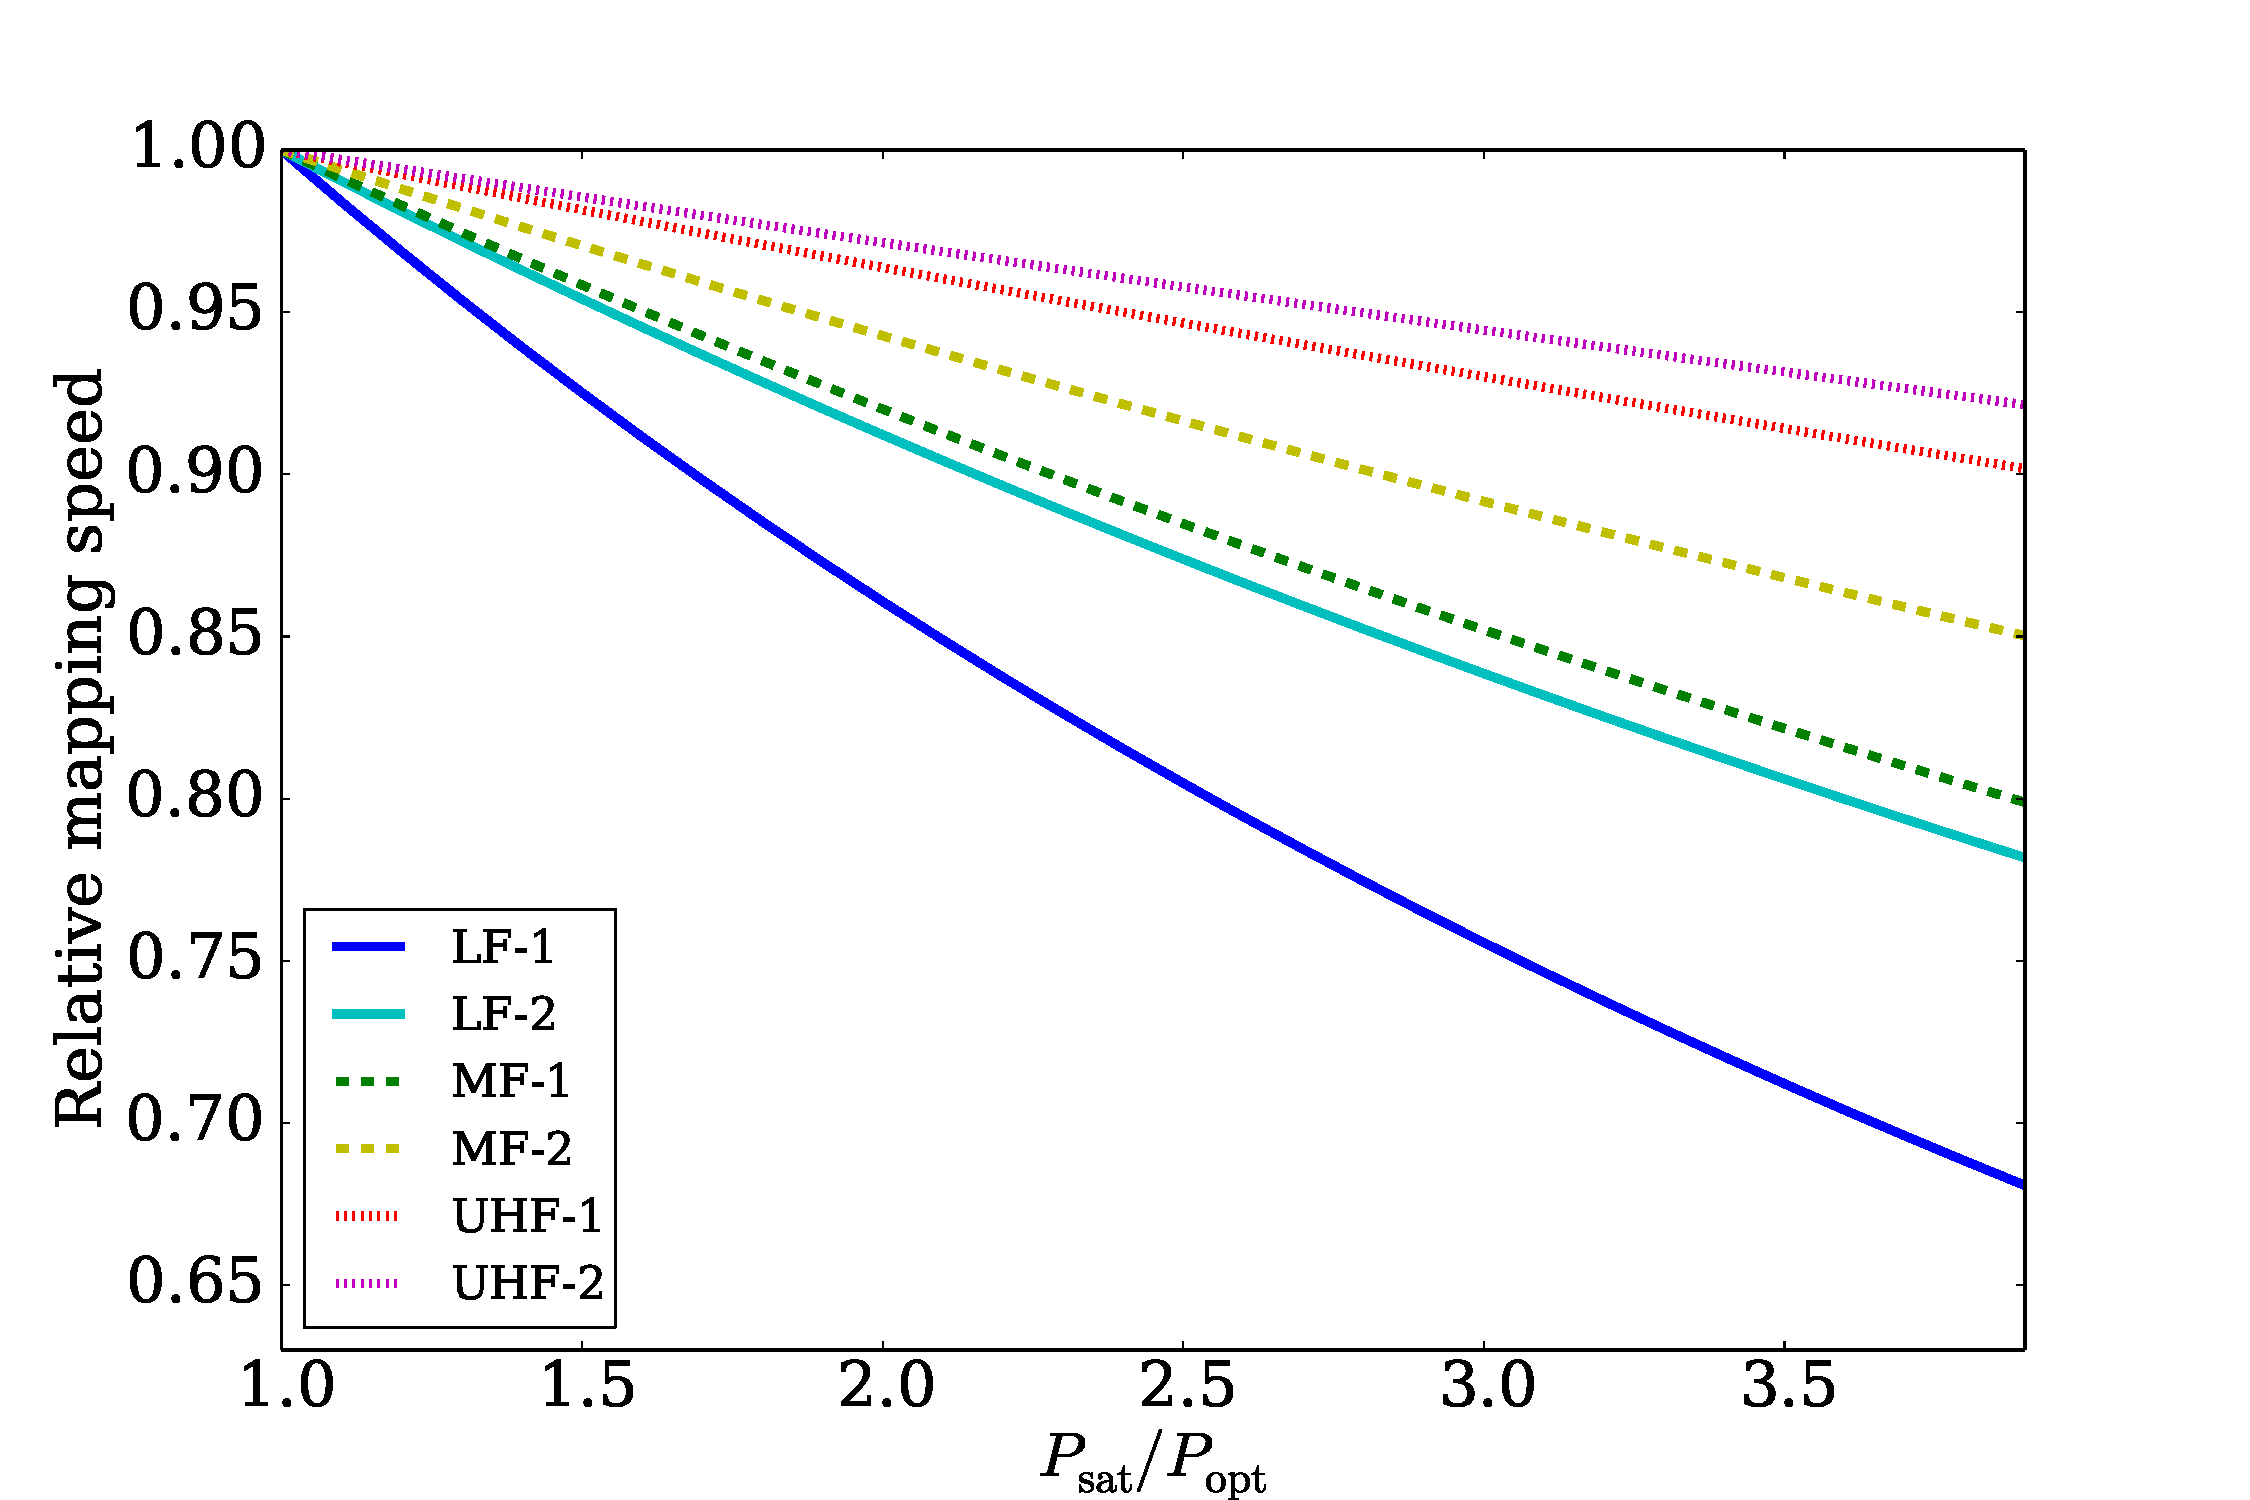
\includegraphics[trim={0.8cm, 0.0cm, 1.5cm, 1.5cm}, clip, width=0.48\linewidth]{BoloCalc/Figures/MSvsPsat_SAC.pdf}}
    \caption{Relative MS for each frequency band in (a) the LAT and (b) the SAT as a function of saturation power $P_{\mathrm{sat}}$, plotted as a fraction of optical power $P_{\mathrm{opt}}$. $P_{\mathrm{sat}}$ impacts MS most at low frequencies, where $NEP_{\mathrm{ph}}$ is smallest, and the impact on the LAT and SAT is similar. The curves for each frequency channel are individually peak-normalized.}
    \label{fig:so_psat}
\end{figure}

%%%%%%%%%%%%%%%%%%%%%%

\subsection{Scan strategy}
\label{sec:scan}

Another application of the sensitivity calculator is to quantify the MS trade-offs of observing at different elevations, PWV values, and with various FOV sizes. These calculations can be used to optimize the map depth achieved using various scan strategies.
%\cite{stevens_so_2018}
BoloCalc utilizes atmospheric simulations of the Cerro Toco Atacama observation site\footnote{Simulations of the South Pole site are also available.} generated by the AM atmospheric modeling code\footnote{\url{https://www.cfa.harvard.edu/~spaine/am/}}, which uses data from the MERRA-2 meteorological reanalysis\footnote{\url{https://gmao.gsfc.nasa.gov/reanalysis/MERRA-2/}} as input. The output from AM produces results consistent with measured sky loading in existing Atacama experiments. The range of input elevations handled by BoloCalc is from 20--90~deg, and the range of input PWV values is from 0--8~mm. 

Figure~\ref{fig:so_scan_strategy} shows normalized LAT MS vs. PWV and elevation in its 90 and 150~GHz bands. The impact of elevation is more prominent in low band, while the impact of water is more prominent in the high band. Additionally, the gradient of MS vs. sky conditions is larger at higher frequency. 

\begin{figure}[!t]
    \subfloat[\label{fig:so_scan_strategy:a}]{
  	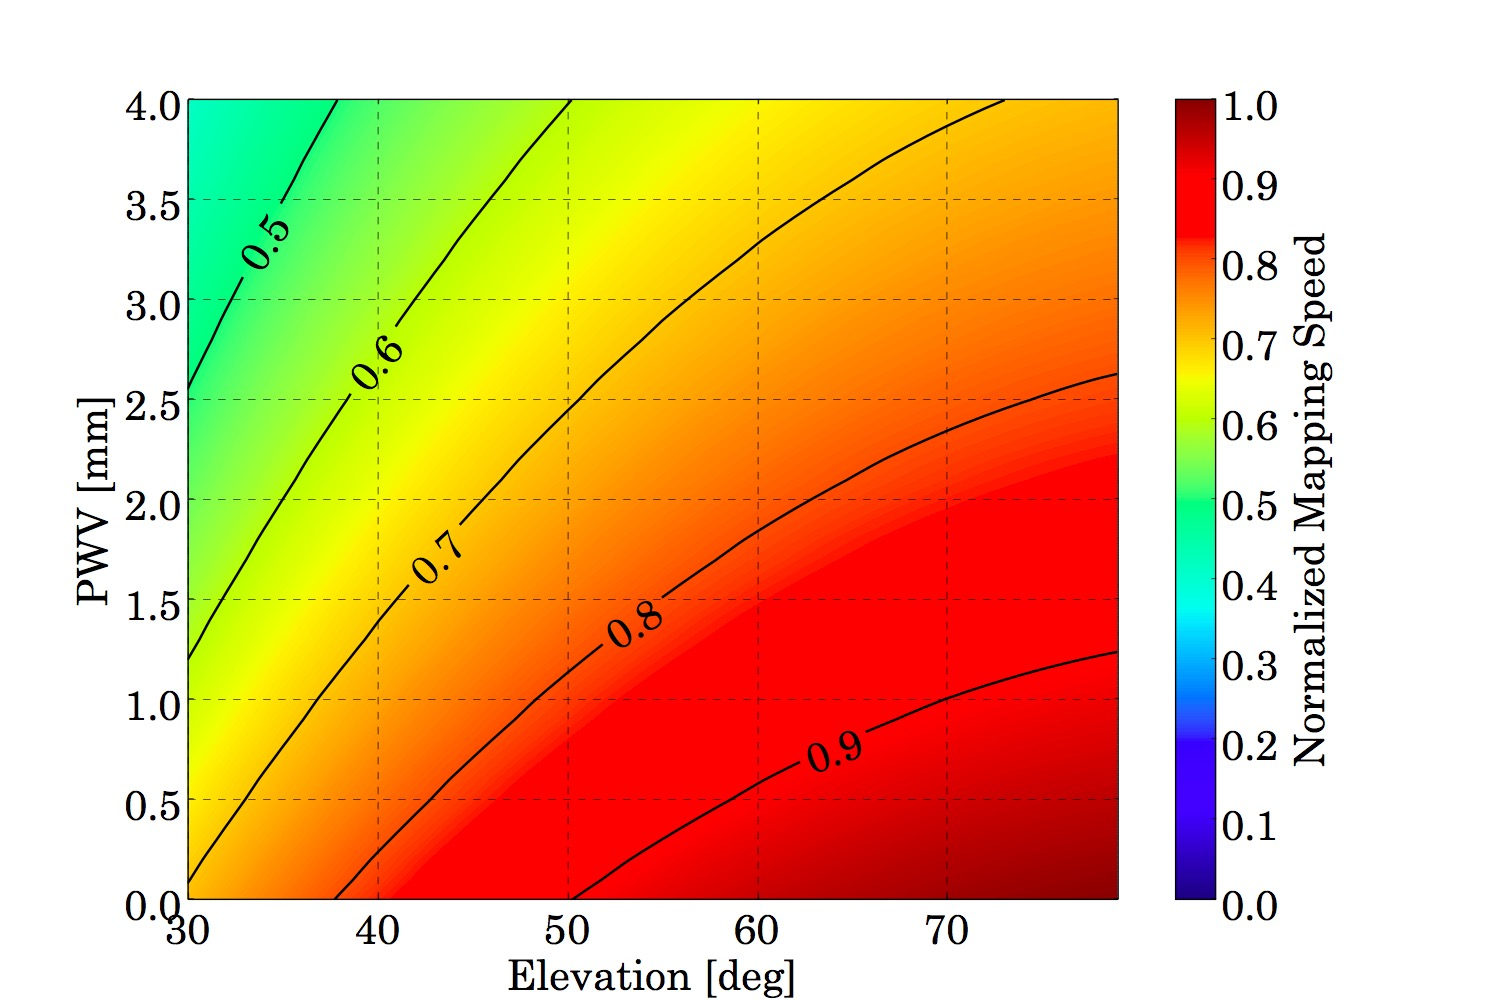
\includegraphics[trim={1.0cm, 0.0cm, 4.0cm, 2.5cm}, clip, width=0.48\linewidth]{BoloCalc/Figures/MSvsATM_90.jpg}}
  	\hfill
    \subfloat[\label{fig:so_scan_strategy:b}]{
  	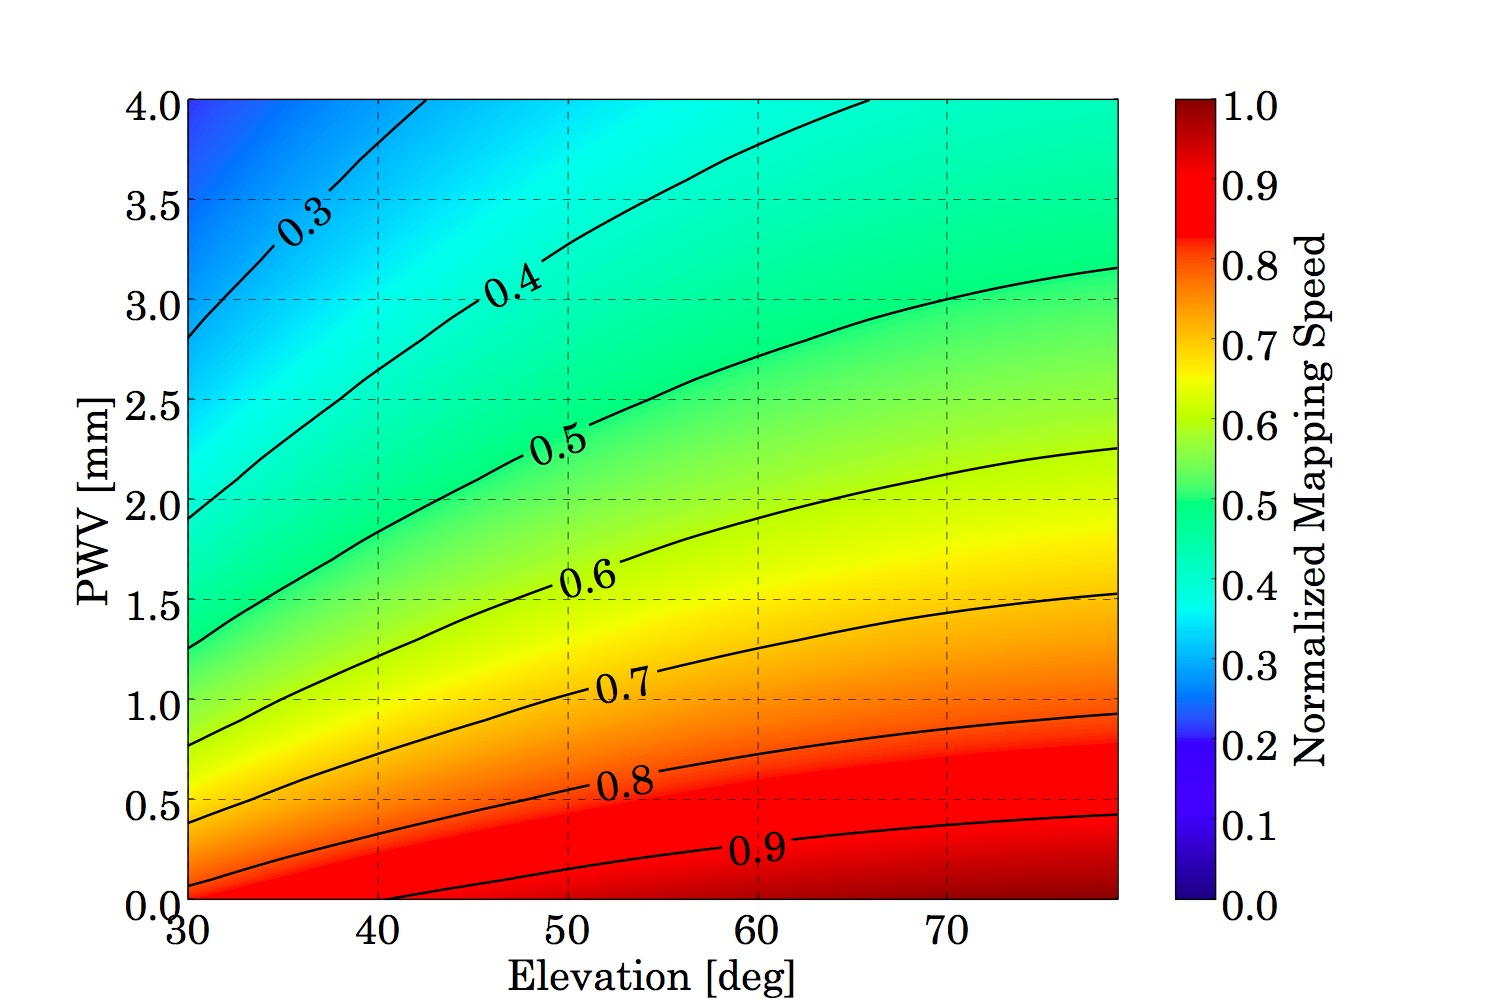
\includegraphics[trim={1.0cm, 0.0cm, 4.0cm, 2.5cm}, clip, width=0.48\linewidth]{BoloCalc/Figures/MSvsATM_150.jpg}}
    \caption{Normalized MS vs. PWV and elevation at the Cerro Toco Atacama observation site in the 90 (a) and 150~GHz (b) bands in the LAT. The impact of elevation is more prominent in the low band, while the impact of water is more prominent in the high band. Additionally, the gradient of MS vs. sky conditions is larger at higher frequency. These tables are easy to generate using BoloCalc and are useful inputs to scan strategy optimization.}
    \label{fig:so_scan_strategy}
\end{figure}

%%%%%%%%%%%%%%%%%%%%%%%%%%%%%%%%
%%%%%%%%%%%%%%%%%%%%%%%%%%%%%%%%
%%%%%%%%%%%%%%%%%%%%%%%%%%%%%%%%

\section{Informing PB-2c Psats}
\label{sec:informing_pb2c_psats}

BoloCalc has also been used extensively to inform the design and characterization of SA. Unlike with SO, for which sensitivity calculations were used to make high-level architectural design choices, the SA design was quite mature by the time of BoloCalc's conception. Therefore, SA has relied on the calculator for lower-level analyses, including to evaluate anti-reflection coatings, readout pathologies, and detector bandpasses. In this section, we highlight BoloCalc's capability to inform these types of hardware considerations by presenting a sensitivity study used to inform PB2c detector saturation power targets.

As discussed in Section~\ref{sec:simons_array_detectors}, saturation power $P_{\mathrm{sat}}$ is the total power conducted from the TES to the thermal bath to which it is weakly connected. $P_{\mathrm{sat}}$ is tunable during the detector fabrication process primarily by tuning the geometry of the thermal link (see Equation~\ref{eq:saturation_power_conductivity}), specifically its $A / l$ ratio. $P_{\mathrm{sat}}$ needs to be large enough to avoid detector saturation but small enough to avoid excess $P_{\mathrm{bias}}$, which in turn leads to excess readout noise (see Equation~\ref{sec:sensitivity_readout_noise}). In other words, $P_{\mathrm{sat}}$ ought not to be too much larger or smaller than the expected optical load $P_{\mathrm{opt}}$. 

The optical load the detector depends on a plethora of factors, including telescope temperature, sky temperature (see Equation~\ref{eq:telescope_temperature_sky_temperature}) telescope optical efficiency, and detector efficiency. While measurements of individual telescope elements can be made in the lab, it is typically difficult to estimate telescope temperature with a high level of precision until the instrument is operating in the field. In a similar manner, the efficiency and bandpass of the detectors is measurable in the lab, but common systematics in Fourier Transform Spectroscopy can make an exact estimate of the on-chip loss difficult. As a result of these realities, the expected $P_{\mathrm{opt}}$ typically has large uncertainties that need to be accounted for when selecting a $P_{\mathrm{sat}}$ target. The optical load on the detectors also depends on weather conditions, which change as function of PWV and telescope boresight elevation. The probability of a given $T_{\mathrm{sky}}$ therefore depends on several factors, including time of year, scan strategy, observation/maintenance cycles, fridge cycle duration, and day-to-day weather patterns.

The goal of selecting an optimal $P_{\mathrm{sat}}$ is one of minimising $N_{\mathrm{\ell}}$ (see Section~\ref{sec:N_ell_mapping_speed}), which is related to mapping speed as
\begin{equation}
    N_{\mathrm{el}} \propto \frac{1}{\mathrm{MS} \; t_{\mathrm{obs}} \eta_{\mathrm{obs}}} \, ,
    \label{eq:bolocalc_N_ell_mapping_speed_relation}
\end{equation}
where $t_{\mathrm{obs}}$ is observation time, $\eta_{\mathrm{obs}}$ is observation efficiency, and MS is mapping speed. Assuming that the lifetime of the experiment is not impacted by the $P_{\mathrm{sat}}$ selection (e.g. that changing detector parameters doesn't require months of re-fabrication!) minimizing power-spectrum noise is analogous to maximizing the $\mathrm{MS} \, \eta_{\mathrm{obs}}$ product.

There are several competing factors when optimizing saturation power:
\begin{enumerate}
    \item Higher $P_{\mathrm{sat}}$ leads to high $\eta_{\mathrm{obs}}$, as it allows you to observe in the presence of higher $T_{\mathrm{sky}}$ and hence larger PWV. A probability density and cumulative probability distribution of PWV during the second season of POLARBEAR observations (2013-2014) is shown in Figure~\ref{fig:pwv_distribution}. As evidenced most clearly by the cumulative probability distribution, PWV is $<$~2.2~mm 80\% of the time and $<$~4~mm 90\% of the time. Conversely, lower $P_{\mathrm{sat}}$ will reduce $\eta_{\mathrm{obs}}$. 
    \item Higher $P_{\mathrm{sat}}$ leads to higher bolometer thermal carrier noise $\mathrm{NEP_{g}}$ and readout noise $\mathrm{NEP_{read}}$ (see Equations~\ref{eq:nep_g} and~\ref{eq:nep_read}), which in turn reduces MS. Conversely, lower $P_{\mathrm{sat}}$ leads to higher MS.
    \item Higher $T_{\mathrm{sky}}$ leads to higher $P_{\mathrm{opt}}$ and hence higher photon noise. Therefore, observations at larger PWV are less sensitive and therefore contribute less \textit{weight} to the final, observation-combined map depth.
\end{enumerate}
Given these factors, the problem of optimizing mapping speed is a problem of estimating $P_{\mathrm{opt}}$ and accurately understanding its scaling with $T_{\mathrm{sky}}$.

%%%%%%%%%%%%%%%%%%%%%%%%%%%%%%%%
%%%%%%%%%%%%%%%%%%%%%%%%%%%%%%%%

\subsection{Estimating $P_{\mathrm{opt}}$}
\label{sec:pb2c_psat_estimating_popt}

According to Equation~\ref{eq:telescope_temperature_sky_temperature}, there are two contributors to optical power on the detector $P_{\mathrm{opt}}$: telescope temperature and sky temperature. Telescope temperature has a distribution that is governed by uncertainties in instrument characterization. In other words, once the telescope is observing in the field, its temperature is relatively constant. Sky temperature, on the other hand, has much smaller uncertainties for a given PWV and elevation but follows a distribution that is governed by weather patterns and scan strategy. For the duration of this study, we assume a constant elevation of 50~deg above the horizon, allowing us to focus on the impact of PWV alone. Probability density functions for PB-2c telescope and sky temperatures are shown in Figure~\ref{fig:pb2c_psat_tel_sky_temp}. The sky temperature distribution traces that of PWV, as expected, while the telescope temperatures are reasonably well described by Gaussian distributions with 95\% confidence intervals of $\pm$~5~$\mathrm{K_{RJ}}$. Uncertainties in telescope temperature are primarily due to uncertainties in the performance of the 220/270~GHz AR coatings.

\begin{figure}[!t]
    \centering
    \subfloat{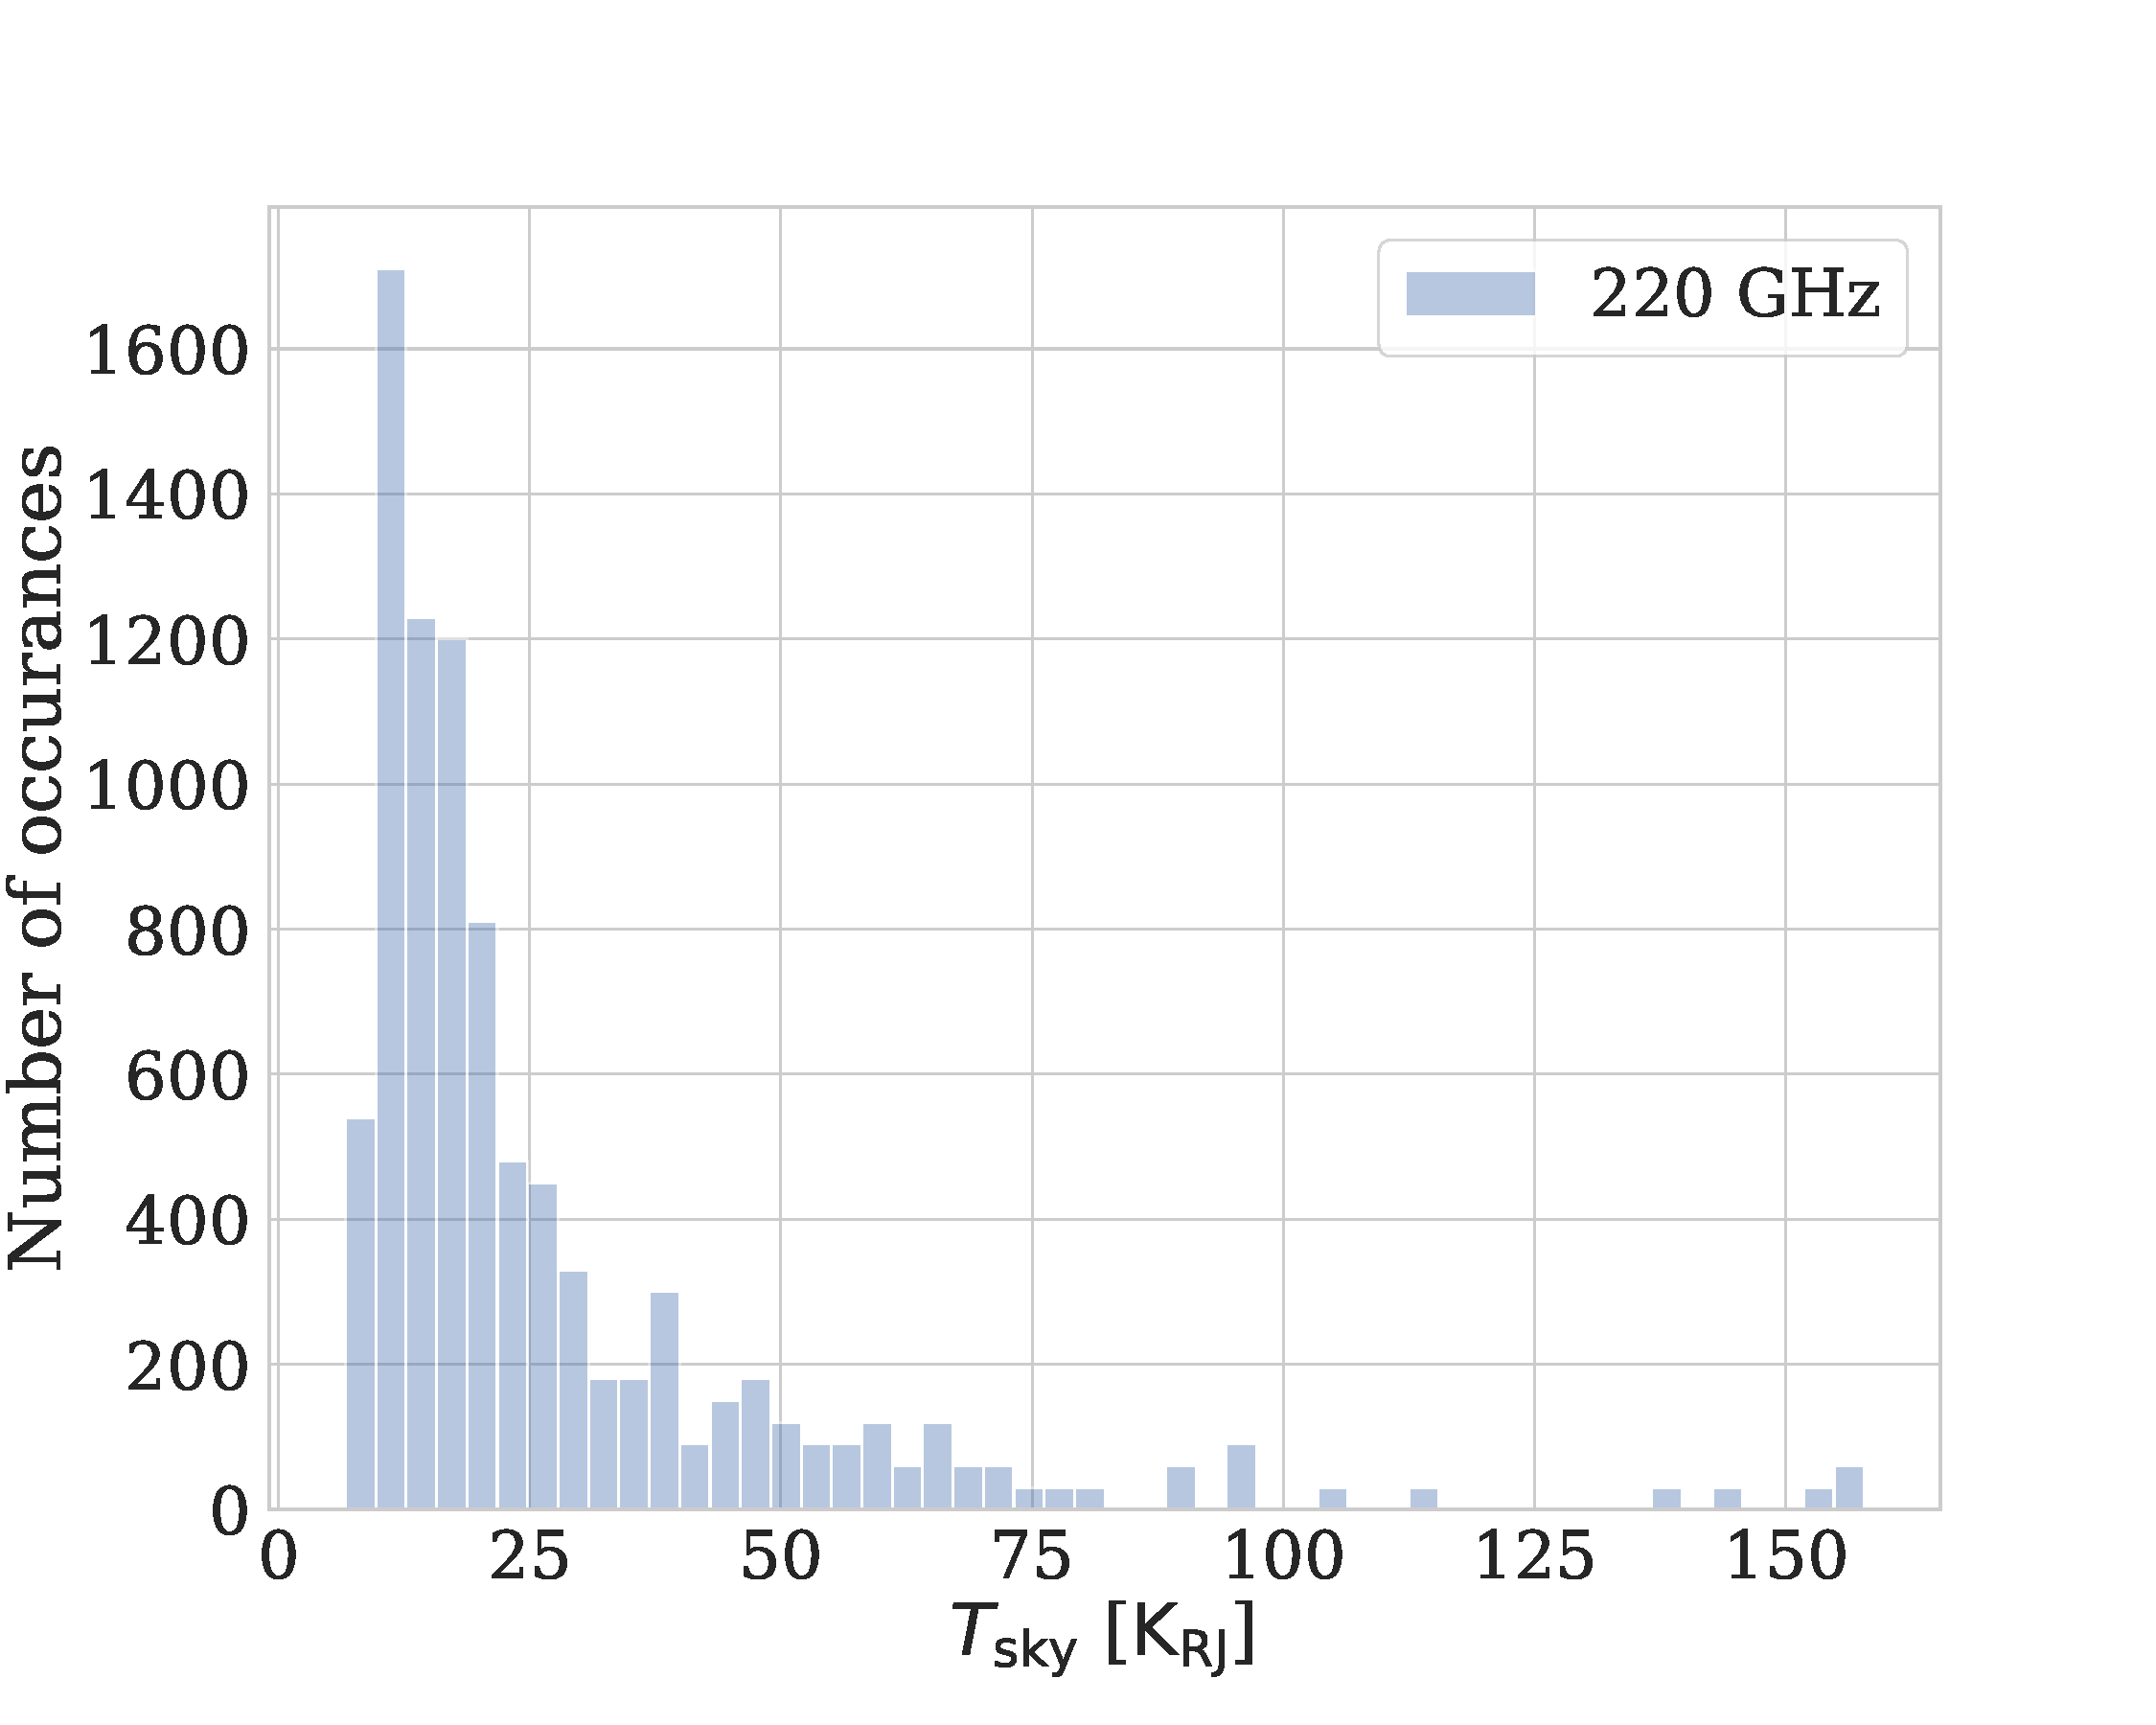
\includegraphics[width=0.48\linewidth, trim=0cm 0cm 0cm 0cm, clip]{BoloCalc/Figures/220_Psat_SkyTemp.pdf}}
    \subfloat{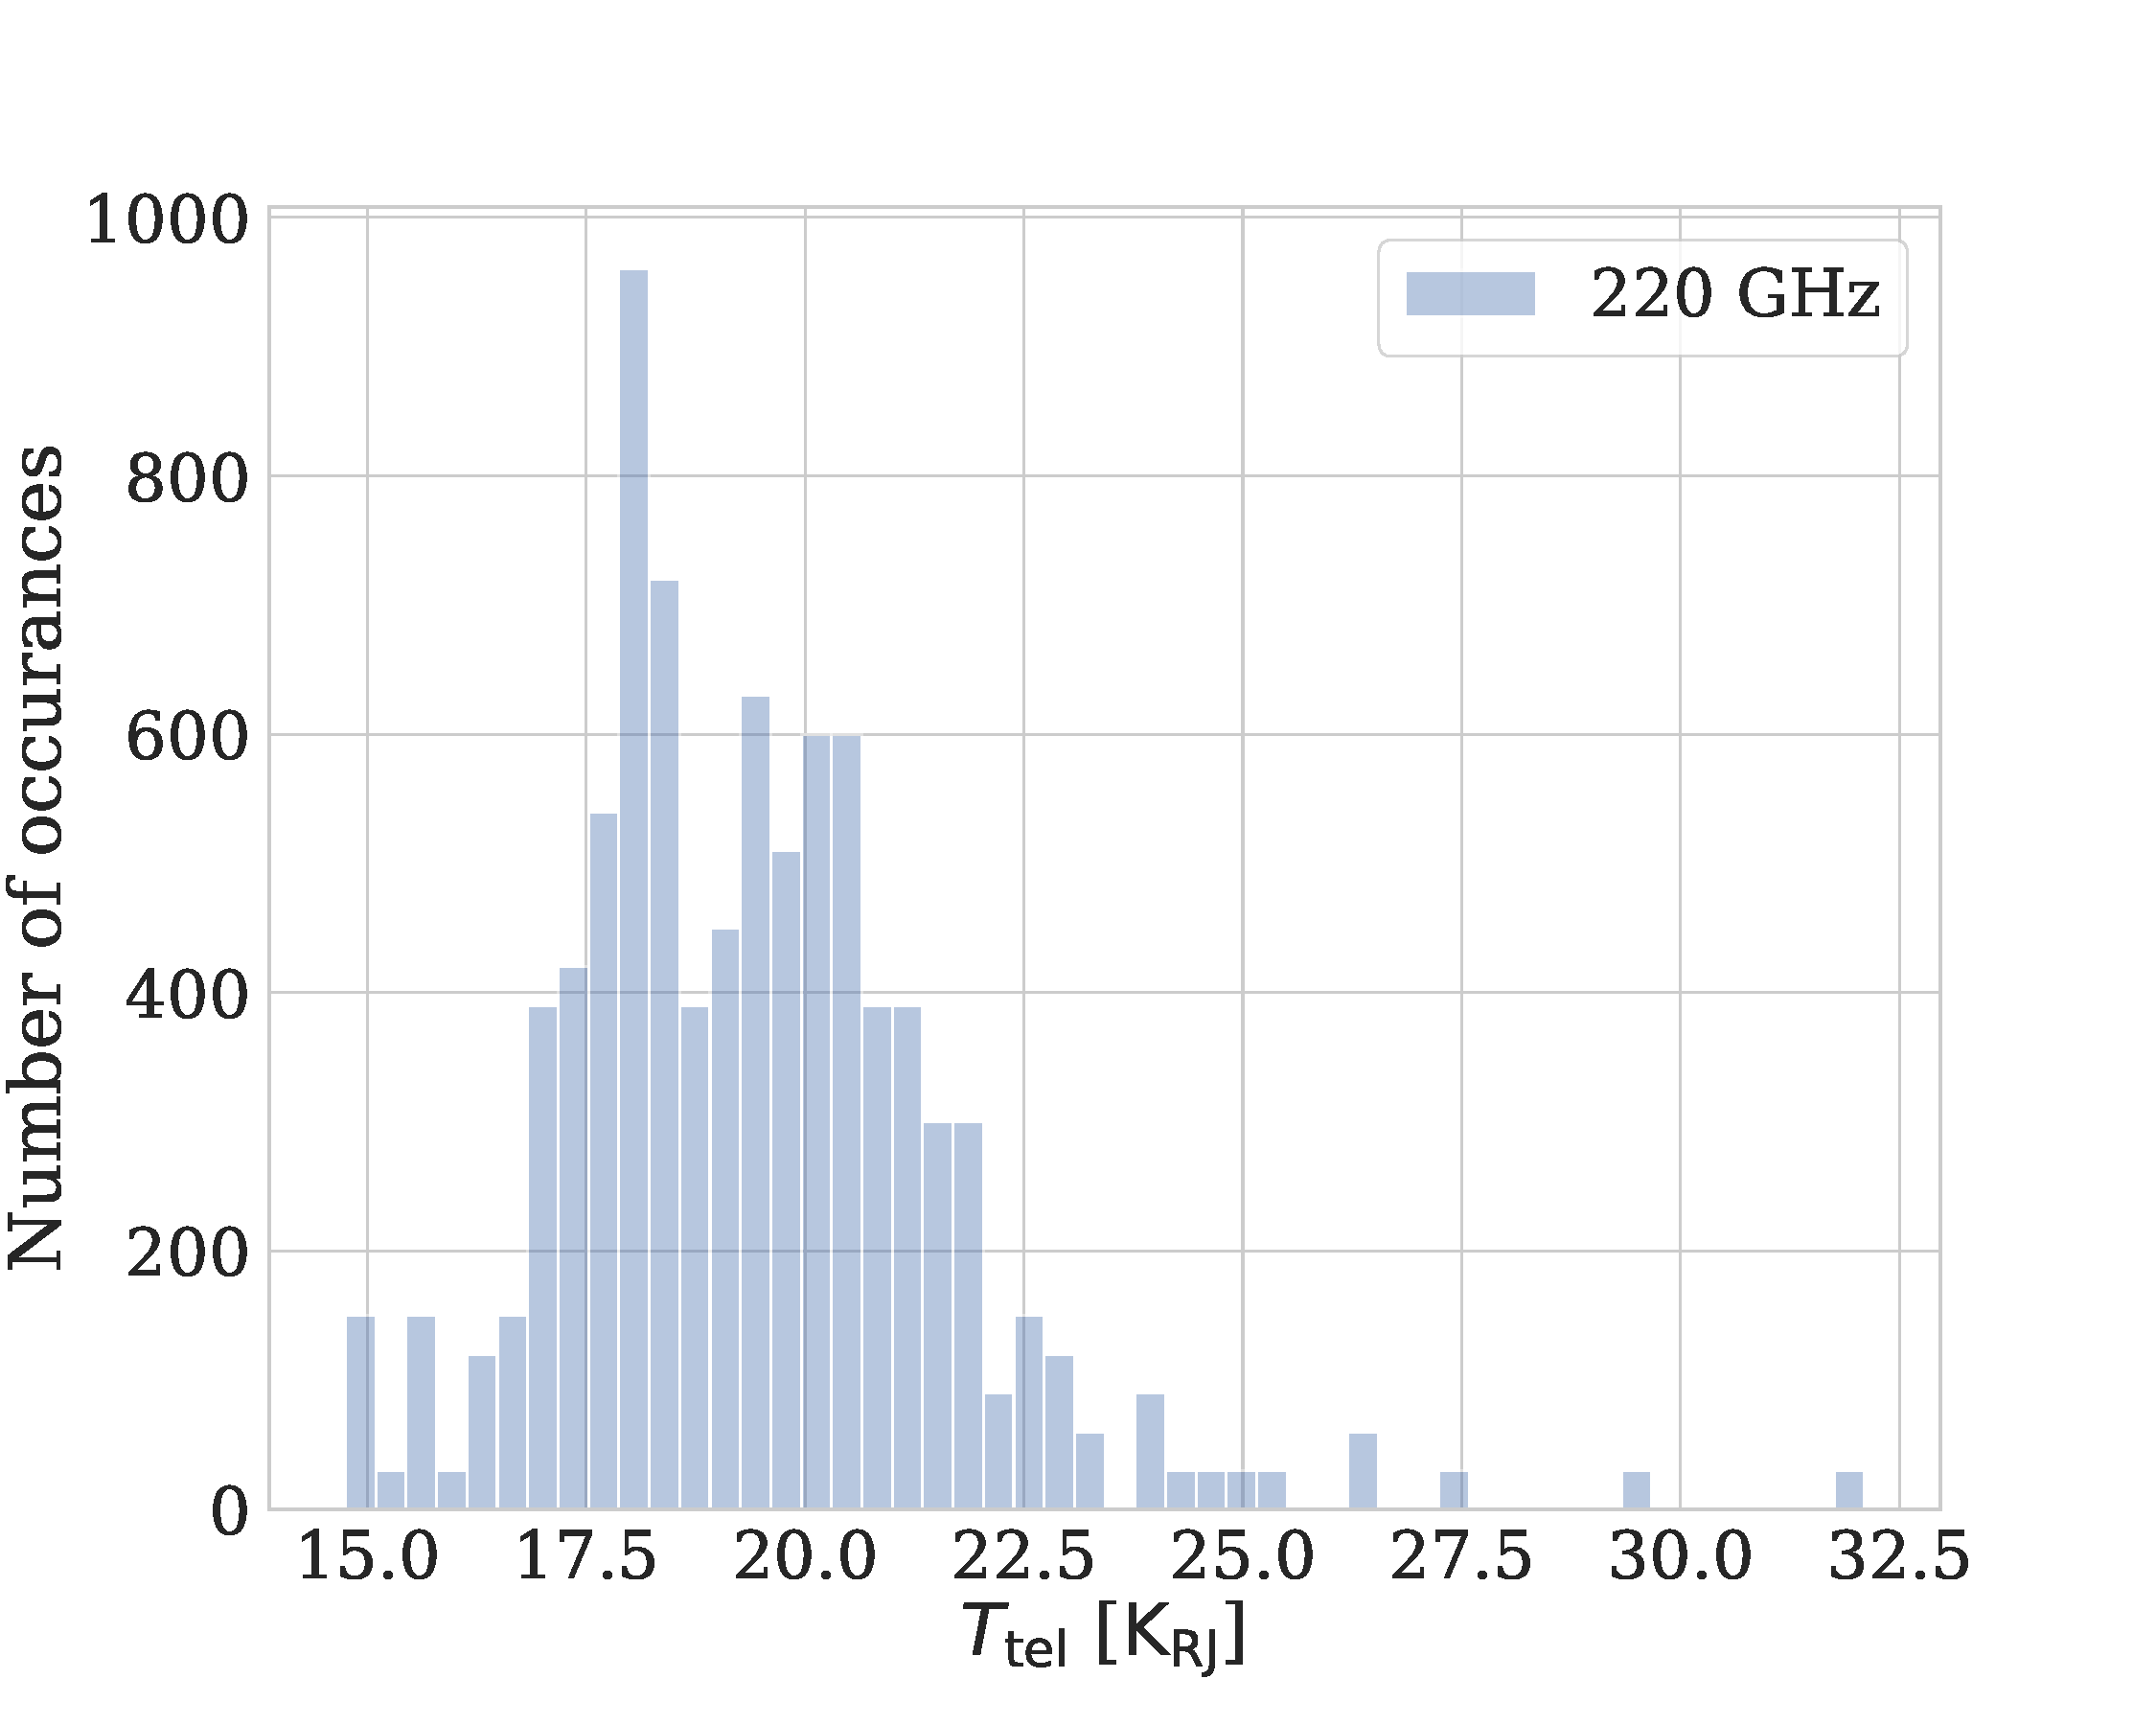
\includegraphics[width=0.48\linewidth, trim=0cm 0cm 0cm 0cm, clip]{BoloCalc/Figures/220_Psat_TelTemp.pdf}}
    \hfill
    \subfloat{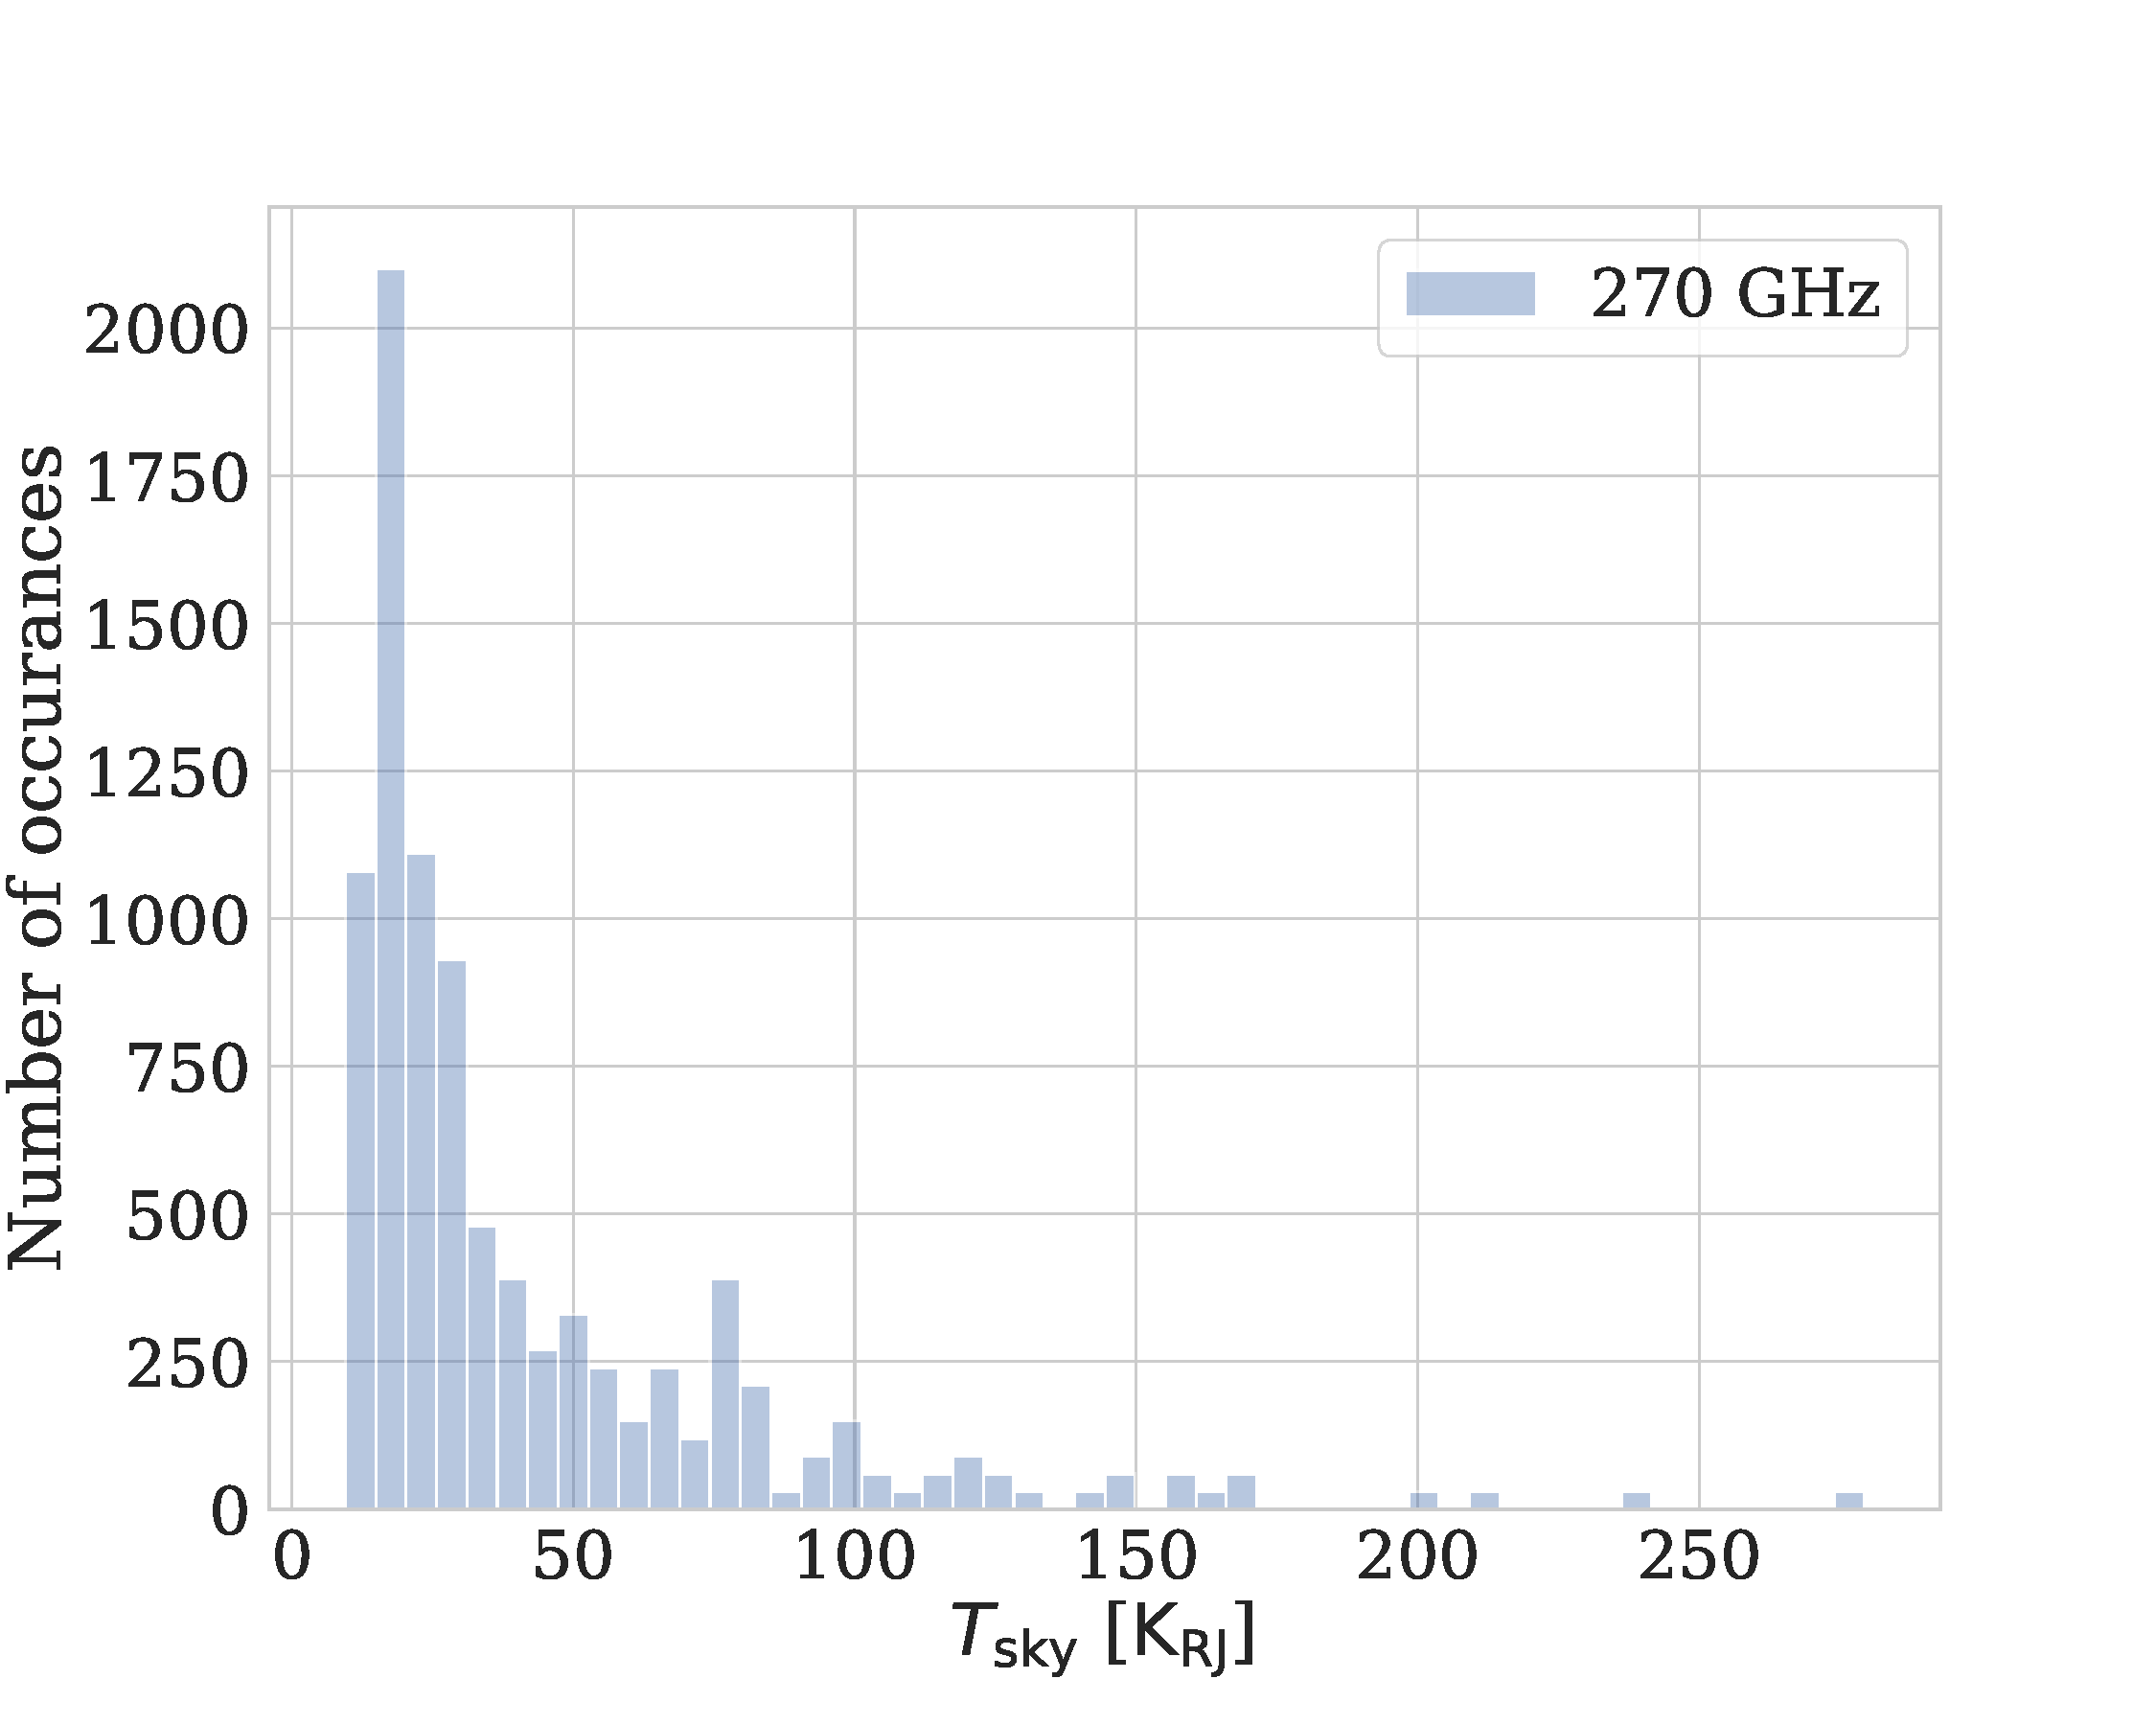
\includegraphics[width=0.48\linewidth, trim=0cm 0cm 0cm 0cm, clip]{BoloCalc/Figures/270_Psat_SkyTemp.pdf}}
    \subfloat{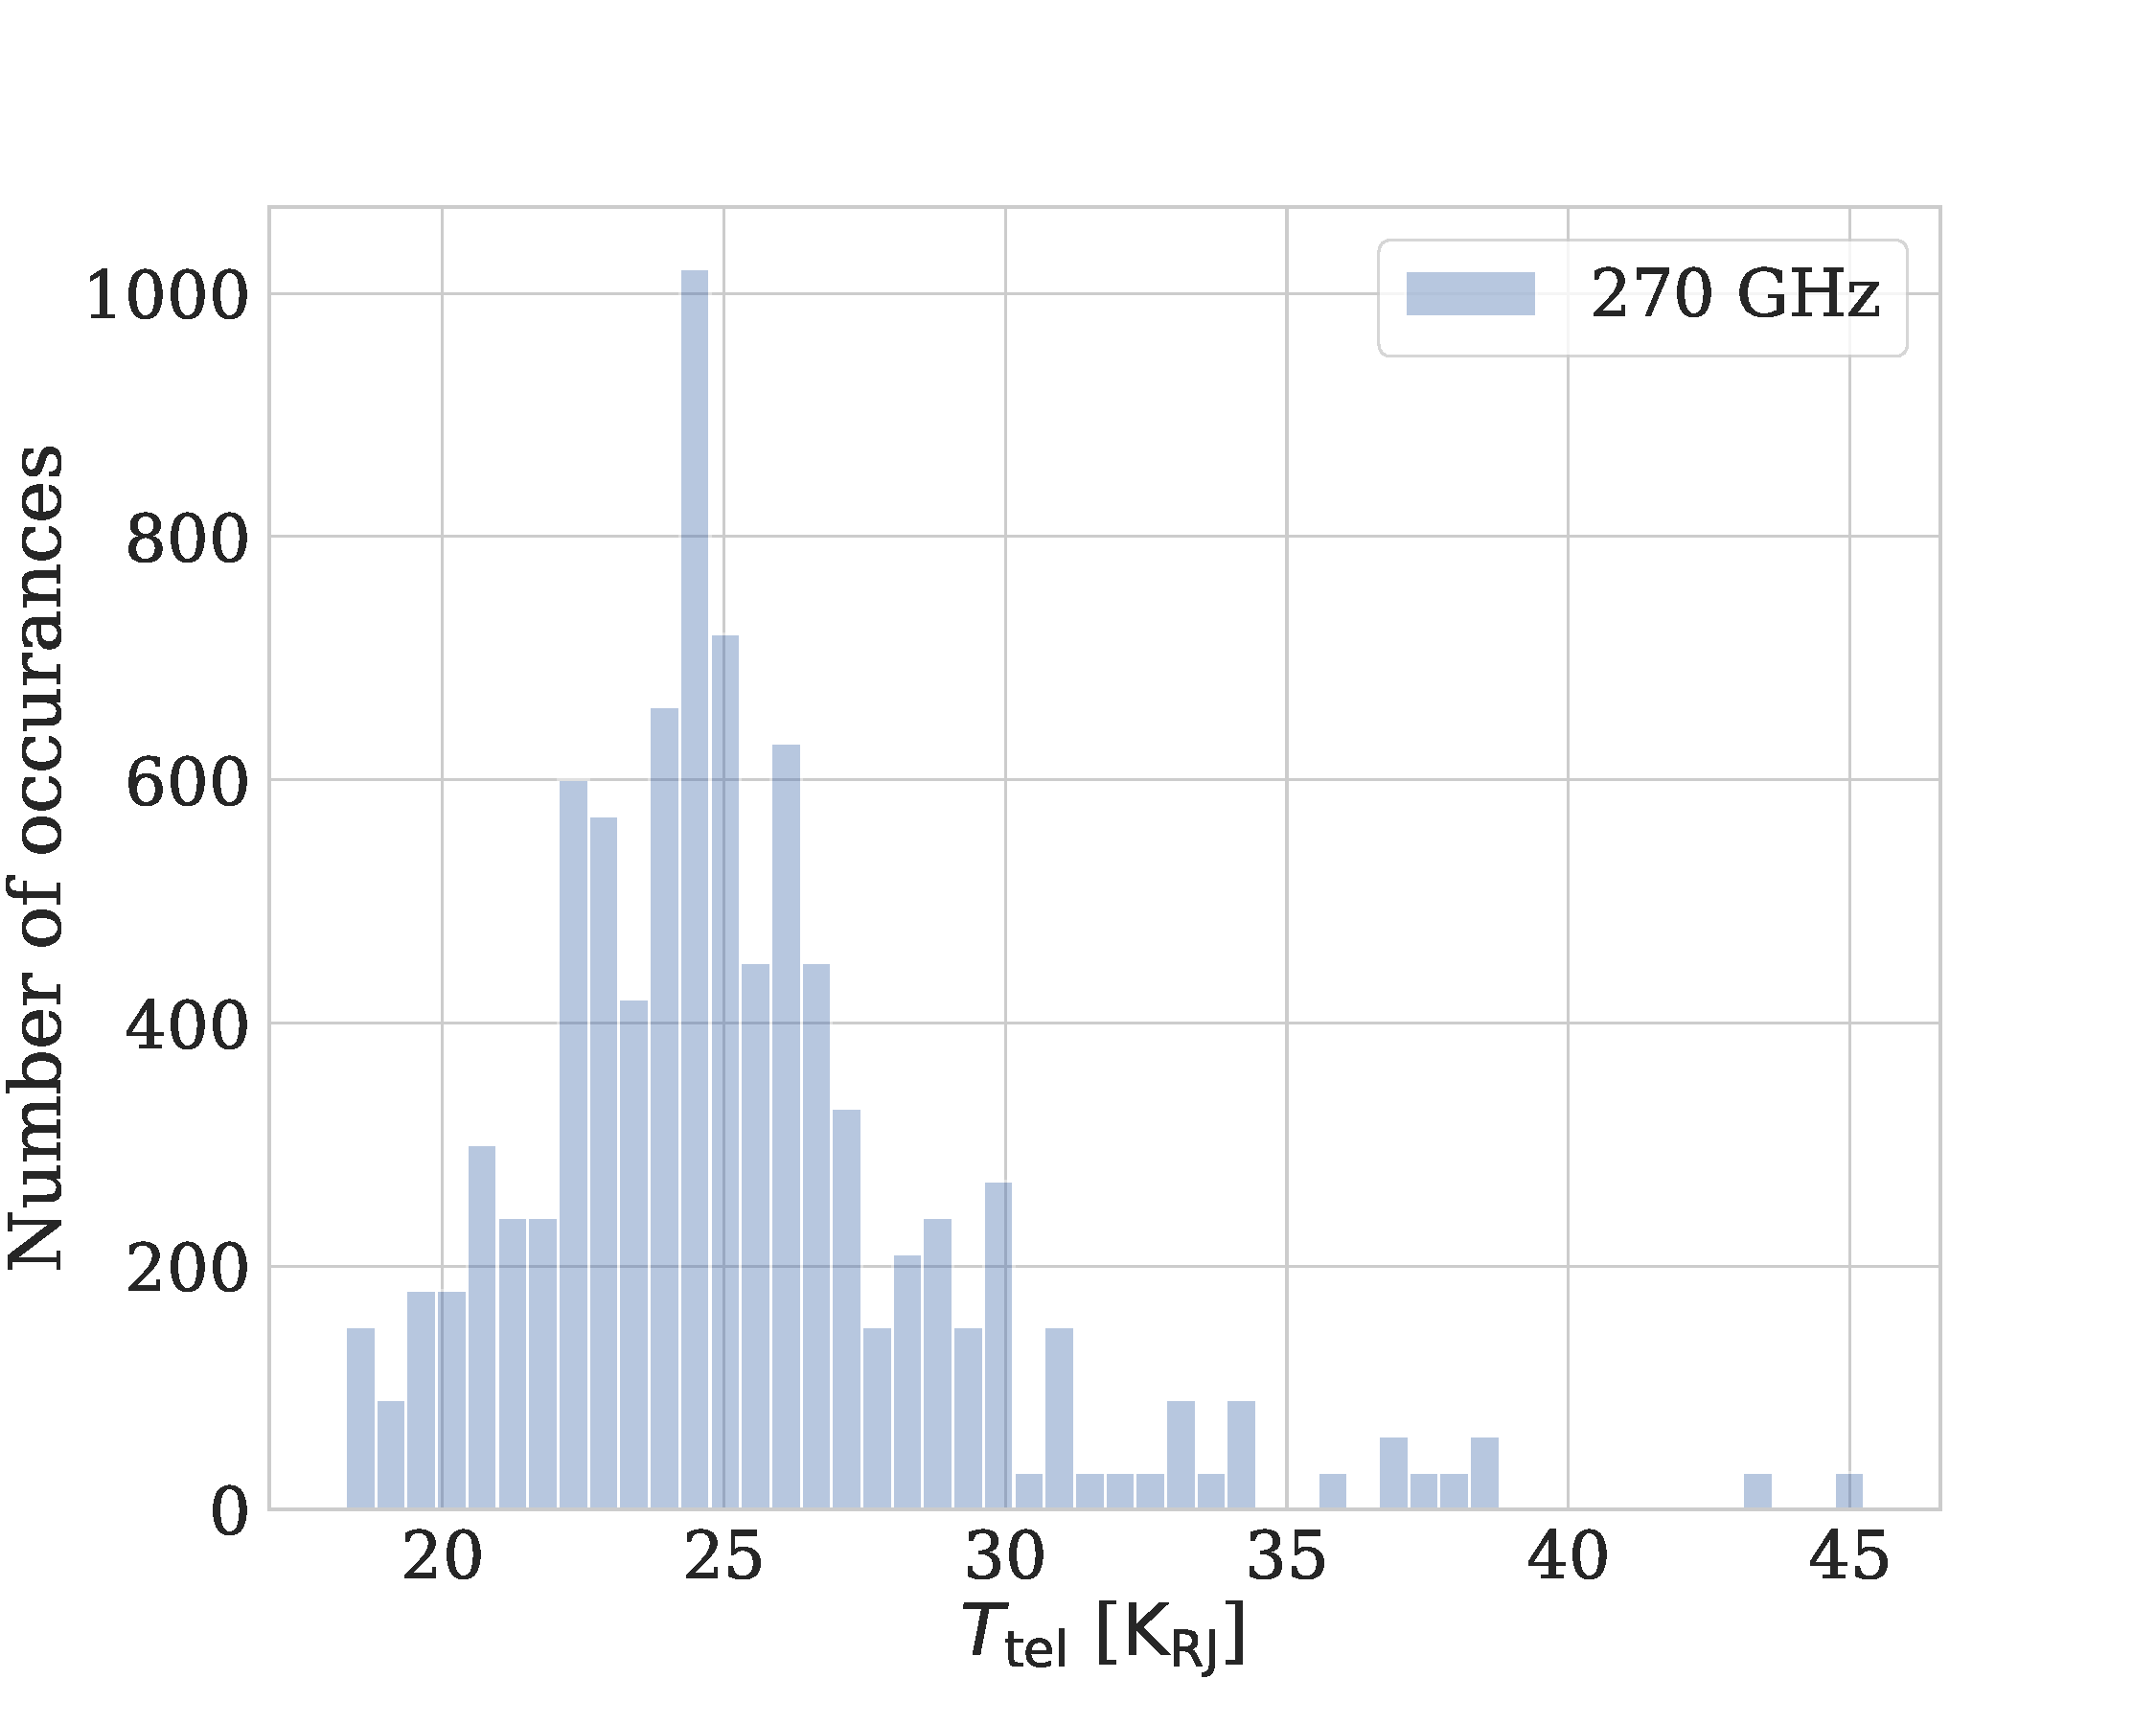
\includegraphics[width=0.48\linewidth, trim=0cm 0cm 0cm 0cm, clip]{BoloCalc/Figures/270_Psat_TelTemp.pdf}}
    \caption{Probability distributions of sky temperature $T_{\mathrm{sky}}$ and telescope temperature $T_{\mathrm{tel}}$ in the PB-2c 220 and 270~GHz bands. A 50~deg telescope boresight elevation is assumed throughout, and therefore the $T_{\mathrm{sky}}$ distributions trade the Atacama PWV distribution shown in Figure~\ref{fig:pwv_distribution}. Variability in telescope temperature is dominated by uncertainties in optical throughput due to lens absorption and on-chip detector loss.}
    \label{fig:pb2c_psat_tel_sky_temp}
\end{figure}


Given probability distributions for $T_{\mathrm{sky}}$ and $T_{\mathrm{tel}}$, we can now use BoloCalc to run thousands of MC realizations of the instrument observing in various weather conditions. Because $P_{\mathrm{opt}} \propto \eta_{\mathrm{det}}$, we decide to break the degeneracy by considering four cases of detector optical efficiency: 20, 40, 60, and 80\%. By doing this delineation, we also provide some intution between the interplay between $P_{\mathrm{sat}}$ $\eta_{\mathrm{det}}$, both of which are governed by the detector fabrication process and are often assessed during the same suite of testing. The resulting $P_{\mathrm{opt}}$ distributions are shown in Figure~\ref{fig:pb2c_popt_cdf}. The distributions are very similar for the two bands are very similar, which might come as a surprise given that atmospheric emission is larger at 270~GHz than at 220. However, as suggested by Equation~\ref{eq:dielectric_emissivity}, absorptivity of dielectric optics increases with frequency, which in turn reduces the telescope's optical throughput. In fact, the worst in-band absorber in the PB-2c cryostat are the alumina lenses, which have an increasing loss tangent with frequency (this quality is what makes alumina an lucrative material for IR absorbing filters), compounding the effect in the 270~GHz band.

\begin{figure}[!t]
    \centering
    \subfloat[\label{fig:pb2c_popt_cdf:a}]{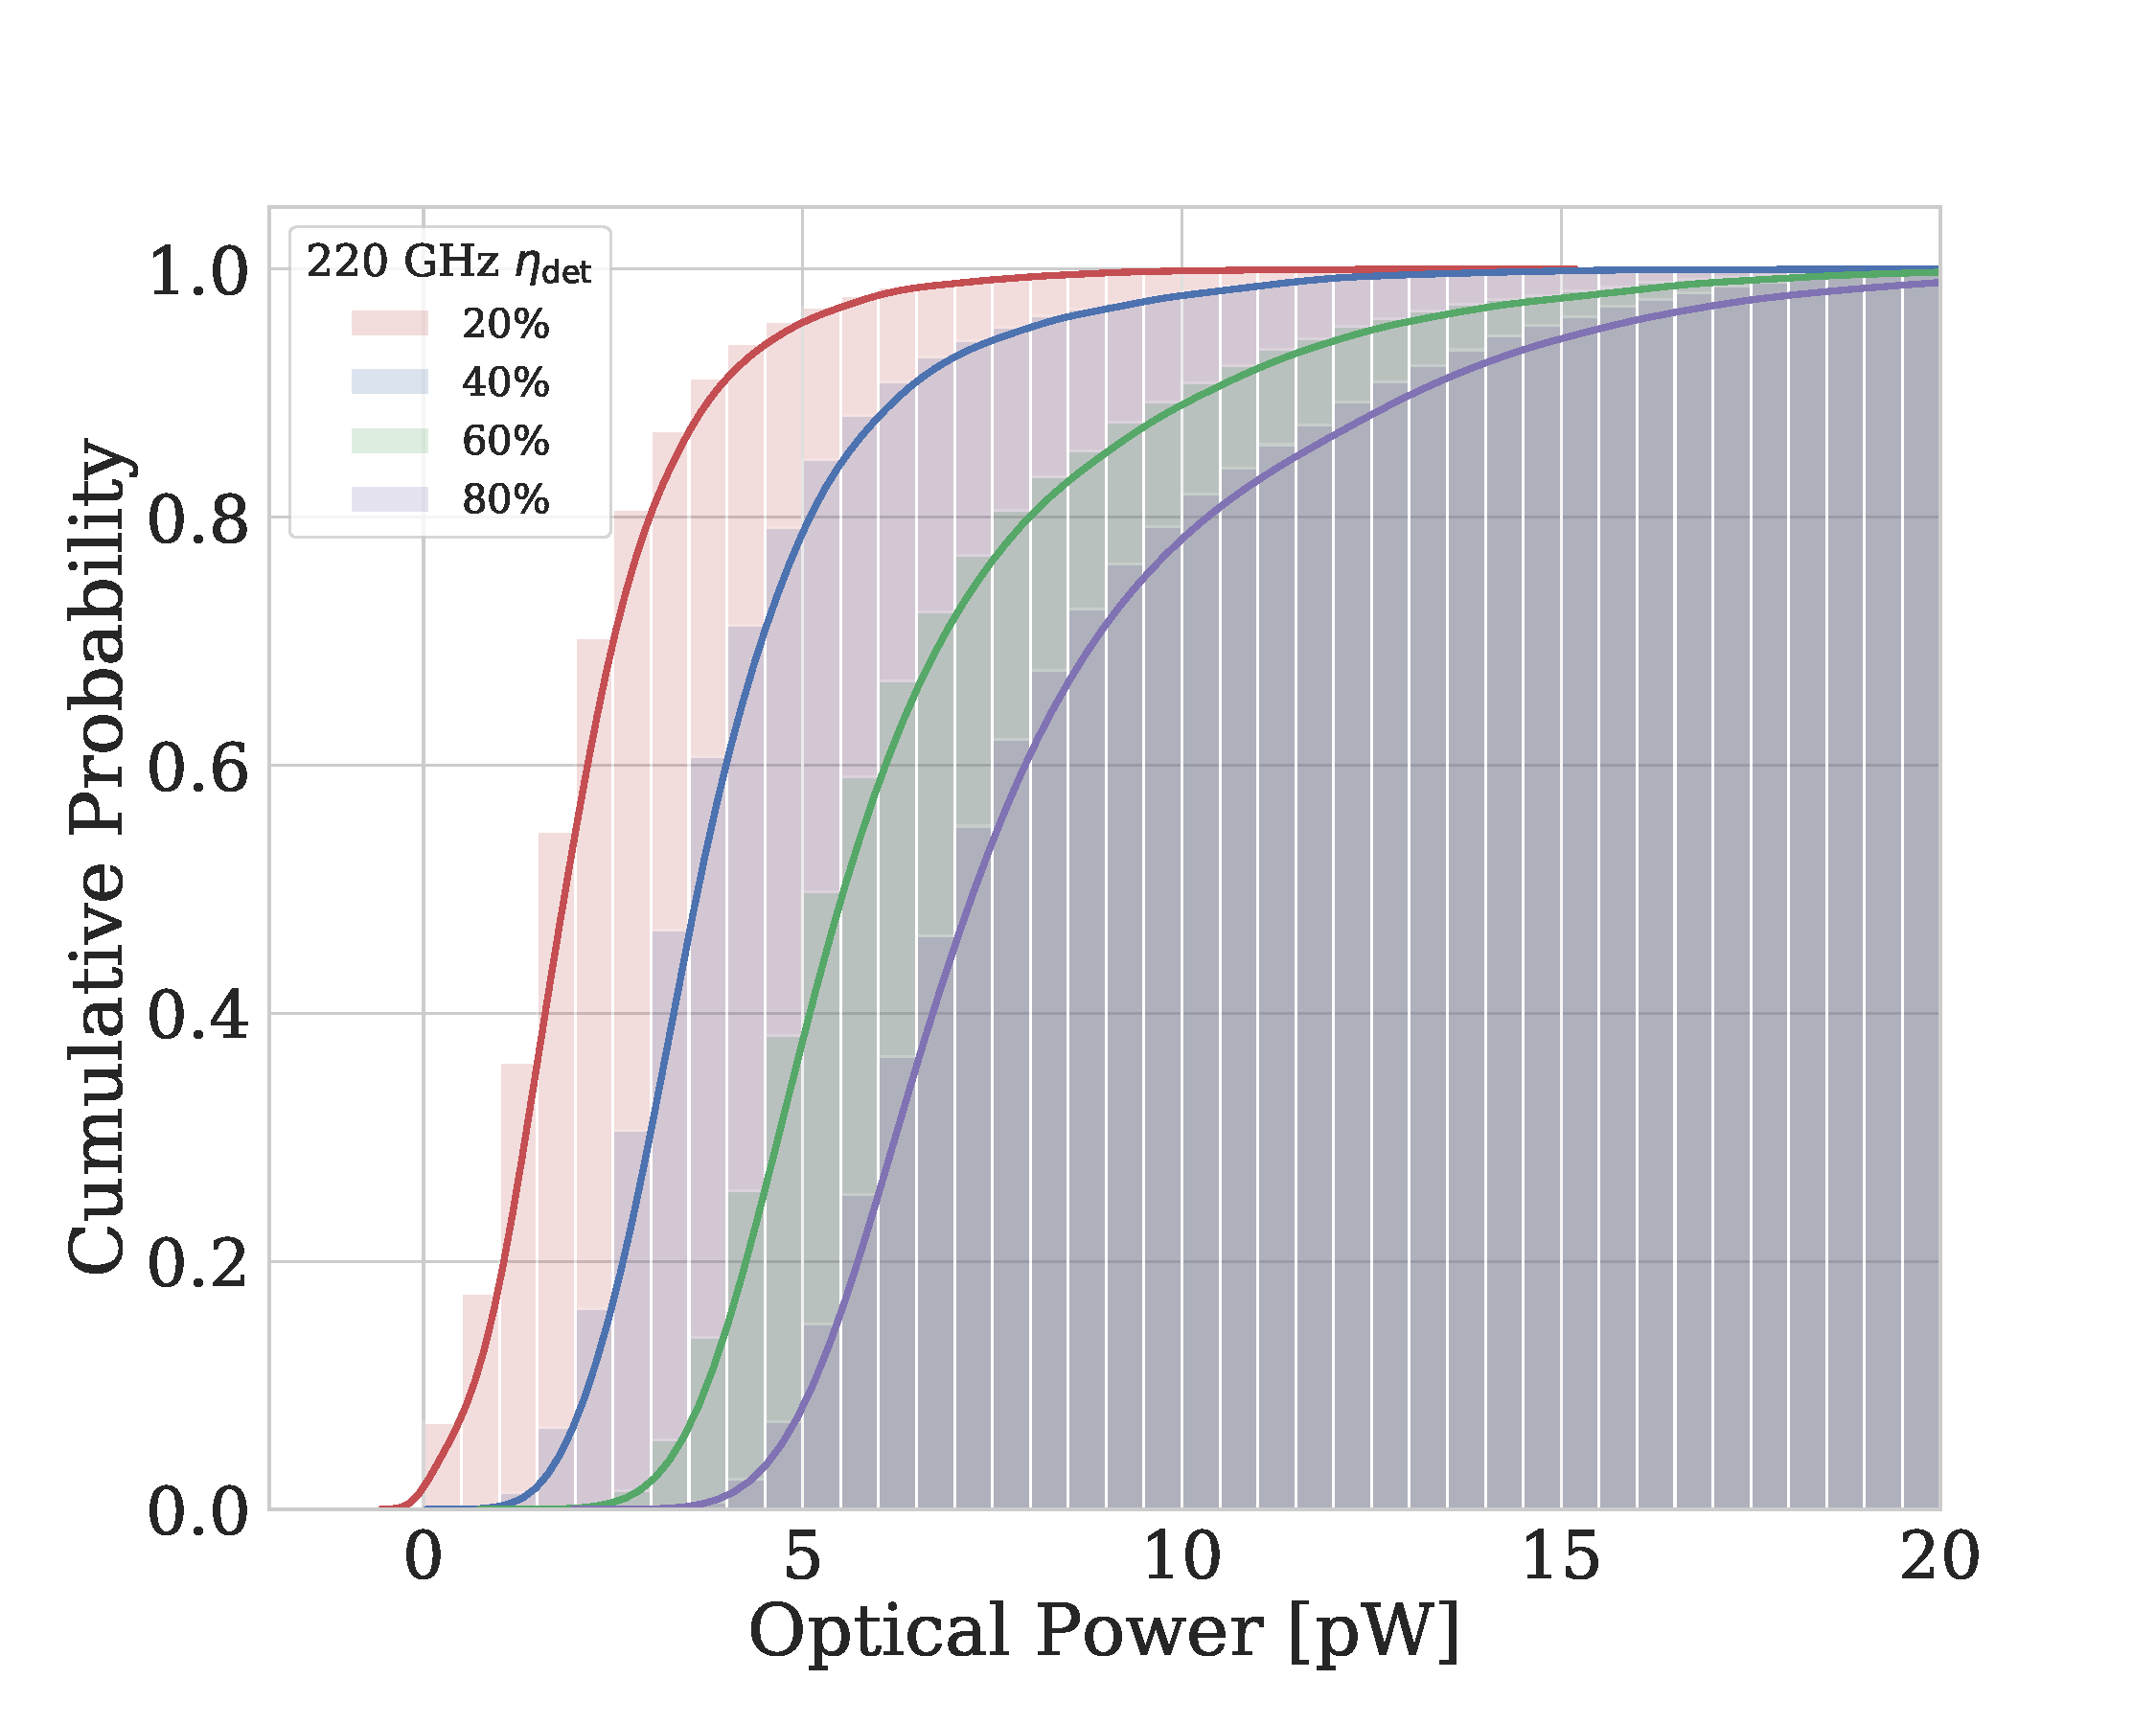
\includegraphics[width=0.48\linewidth, trim=0cm 0cm 0cm 0cm, clip]{BoloCalc/Figures/220_Psat_Popt_CDF_all.pdf}}
    \subfloat[\label{fig:pb2c_popt_cdf:b}]{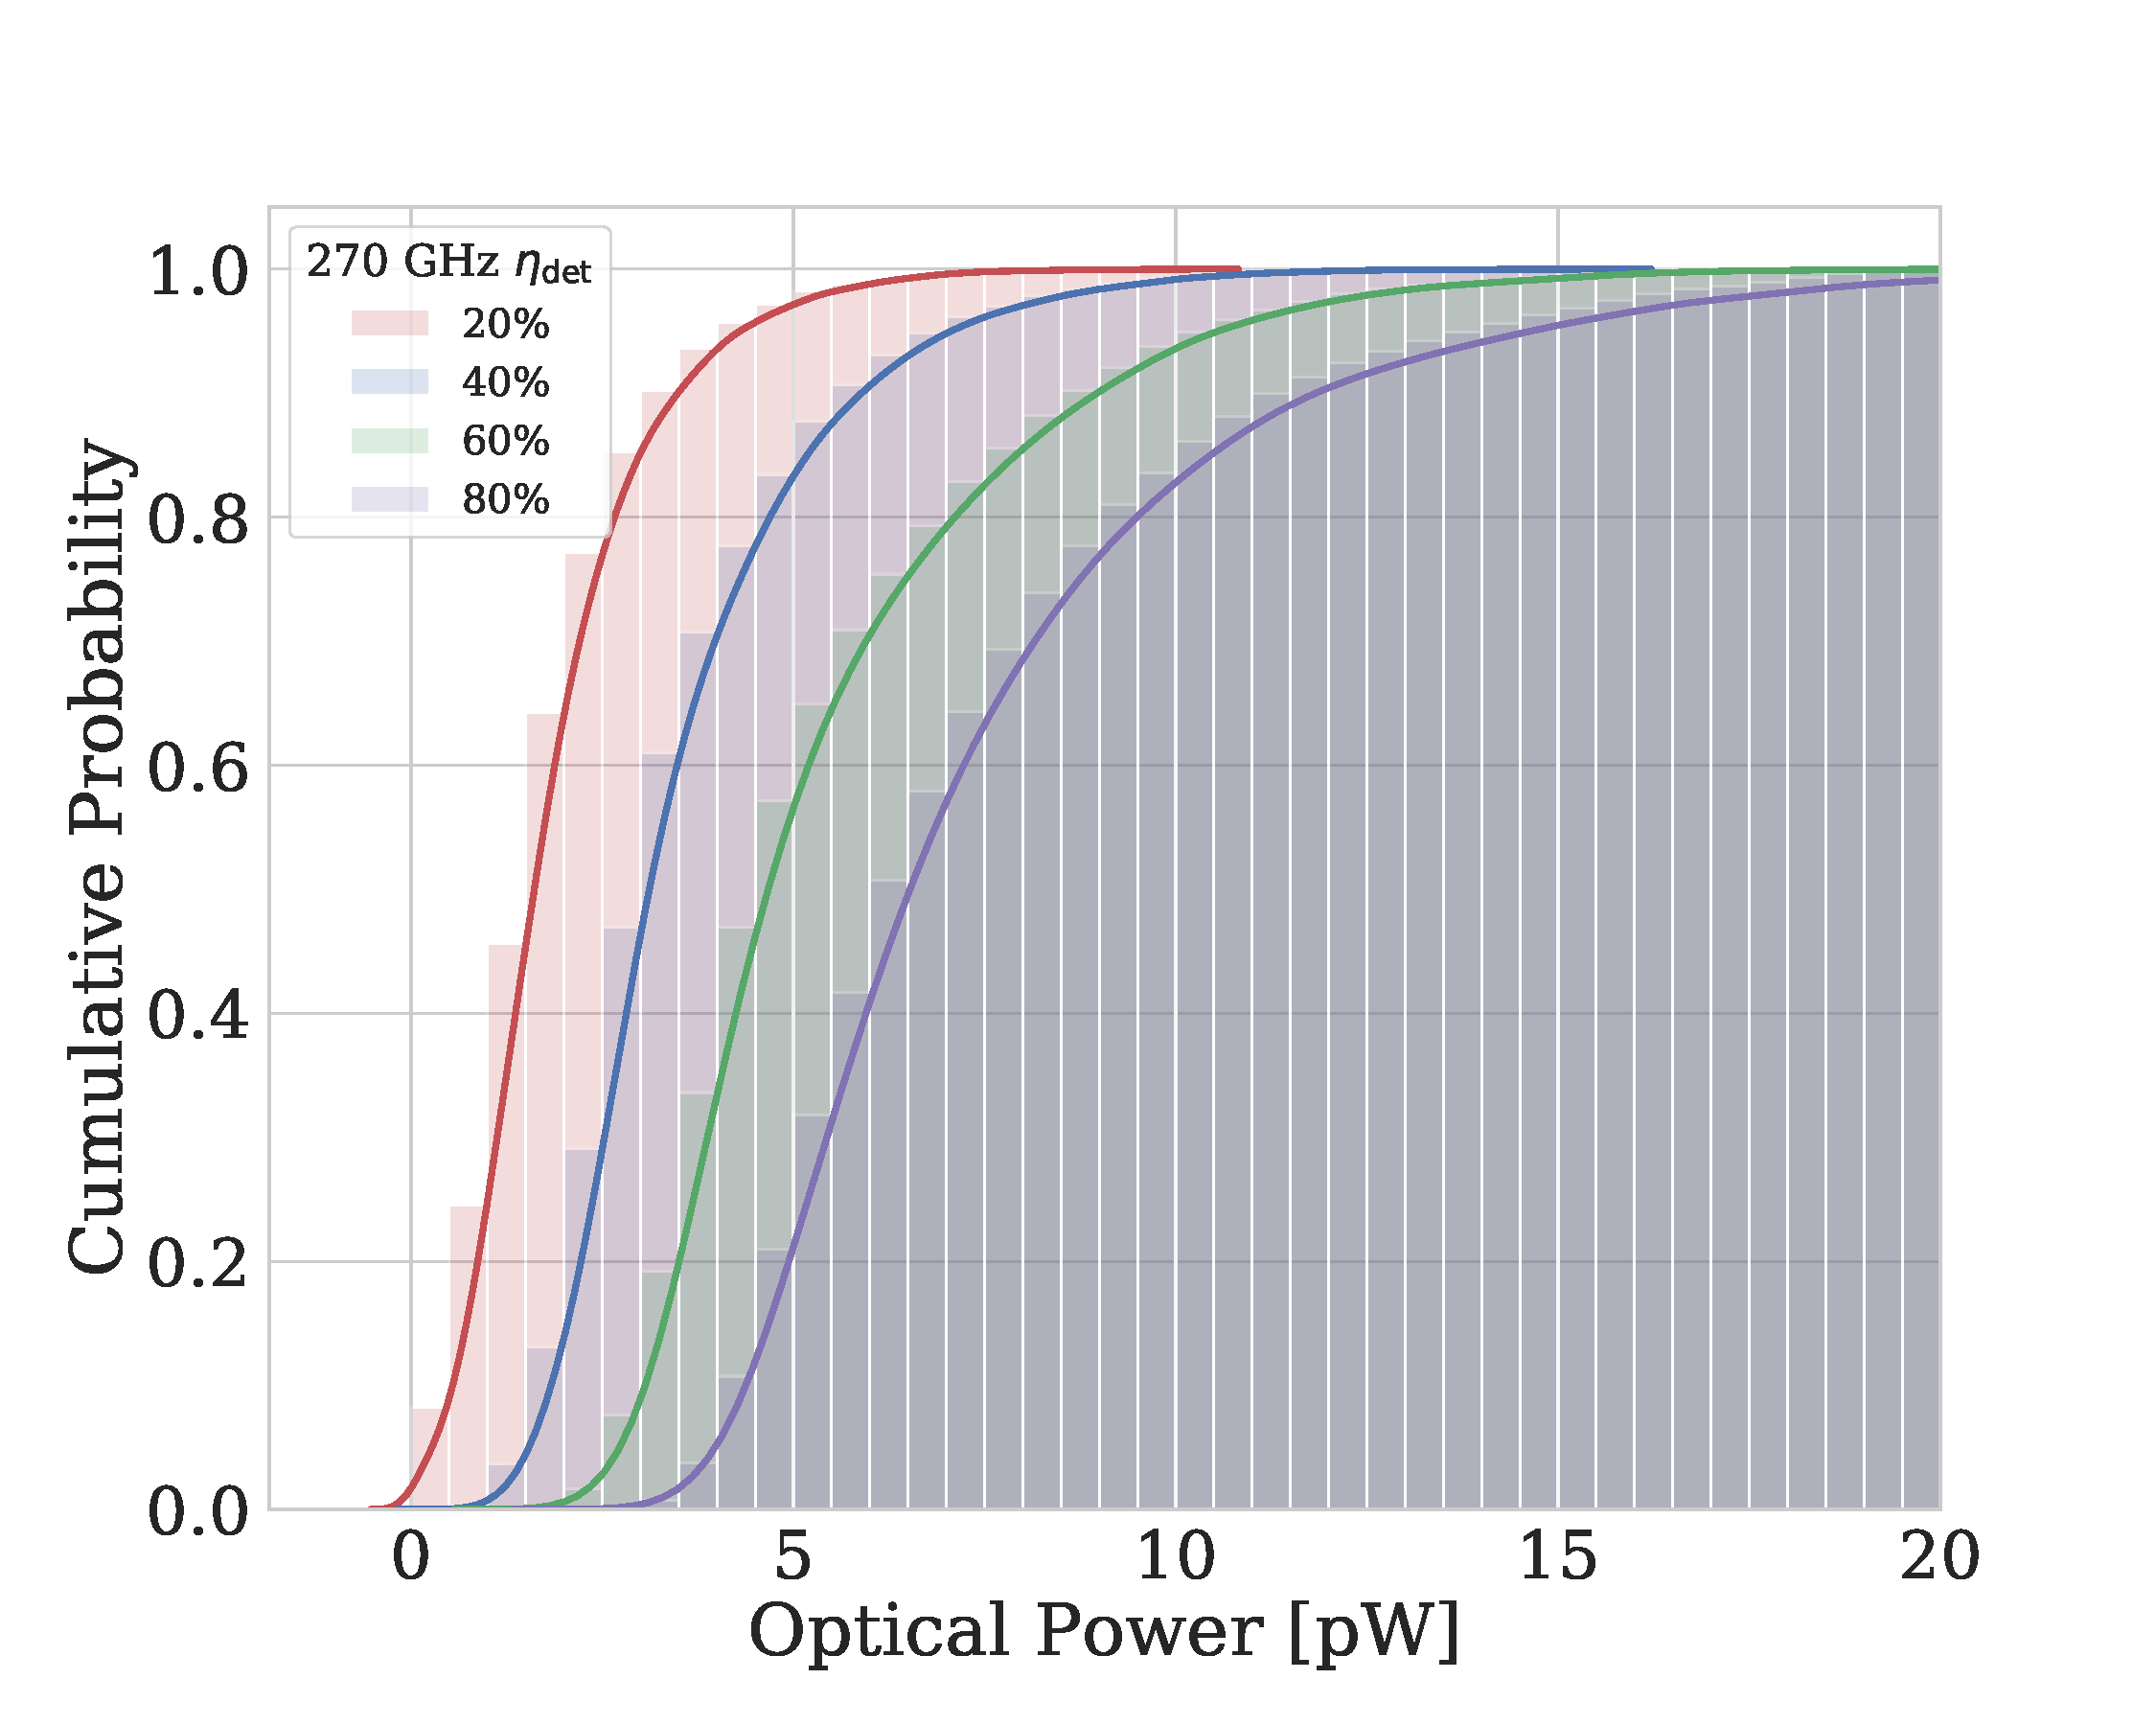
\includegraphics[width=0.48\linewidth, trim=0cm 0cm 0cm 0cm, clip]{BoloCalc/Figures/270_Psat_Popt_CDF_all.pdf}}
    \caption[Expected optical power for PB2c in both the 220 and 270 GHz bands as simulated by BoloCalc]{\ref{fig:pb2c_popt_cdf:a} shows a historgram of the expected optical power in the 220 GHz band on PB2c given undertainties in dewar temperature, sky power, and detector bandpass, assuming a detector efficiency of 60\%. \ref{fig:pb2c_popt_cdf:b} shows the same histogram but for the 270 GHz band. The solid line denotes the median, and the dashed and dotted lines represent the 68\% and 95\% confidence levels, respectively. These plots demonstrate BoloCalc's ability to fold uncertainties in instrument parameters into the expected measured values.}
    \label{fig:pb2c_popt_cdf}
\end{figure}

It is worth emphasizing that the distributions in Figure~\ref{fig:pb2c_popt_cdf} fold uncertainties in the instrument configuration in with variations in sky load. Therefore, this plot can be thought of as the load for deploying an MC-generated instrument to observe an MC-generated sky. Another possible approach would be to handle the $T_{\mathrm{sky}}$ and $T_{\mathrm{tel}}$ separately in order to apply different observation strategies for different telescope realizations. Such an approach is reasonable, as the observation strategy can be tuned after learning about the instrument in the field. Such an analysis is involves too many details and independent variables for the PB-2c discussion, which was meant to quickly feedback to detector fabrication efforts. That said, BoloCalc is fully capable of running such parameter separations, and such a study may be interesting for other maturing experiments such as SO.

%%%%%%%%%%%%%%%%%%%%%%%%%%%%%%%%
%%%%%%%%%%%%%%%%%%%%%%%%%%%%%%%%

\subsection{Maximizing $\mathrm{MS} \times \eta_{\mathrm{opt}}$}
\label{sec:pb2c_psat_maximizing_ms}

Armed with optical power cumulative distributions in Figure~\ref{fig:pb2c_popt_cdf}, we are now in a position to calculate mapping speed as a function of both detector efficiency $\eta_{\mathrm{det}}$ and saturation power $P_{\mathrm{sat}}$. Figure~\ref{fig:pb2c_psat_ms} shows peak-normalized \textit{median} mapping speed vs $P_{\mathrm{sat}}$ in both the 220 and 270~GHz. As expected, mapping speed decreases with increasing saturation power, and the impact is larger for smaller detector efficiency $\eta_{\mathrm{det}}$, for which $\mathrm{NEP_{ph}}$ is smaller but $\mathrm{NEP_{read}}$ is larger. Because the $P_{\mathrm{opt}}$ distributions in Figure~\ref{fig:pb2c_popt_cdf} are similar, so are the mapping speed vs saturation power curves.

\begin{figure}
    \centering
    \subfloat[\label{fig:pb2c_psat_ms:a}]{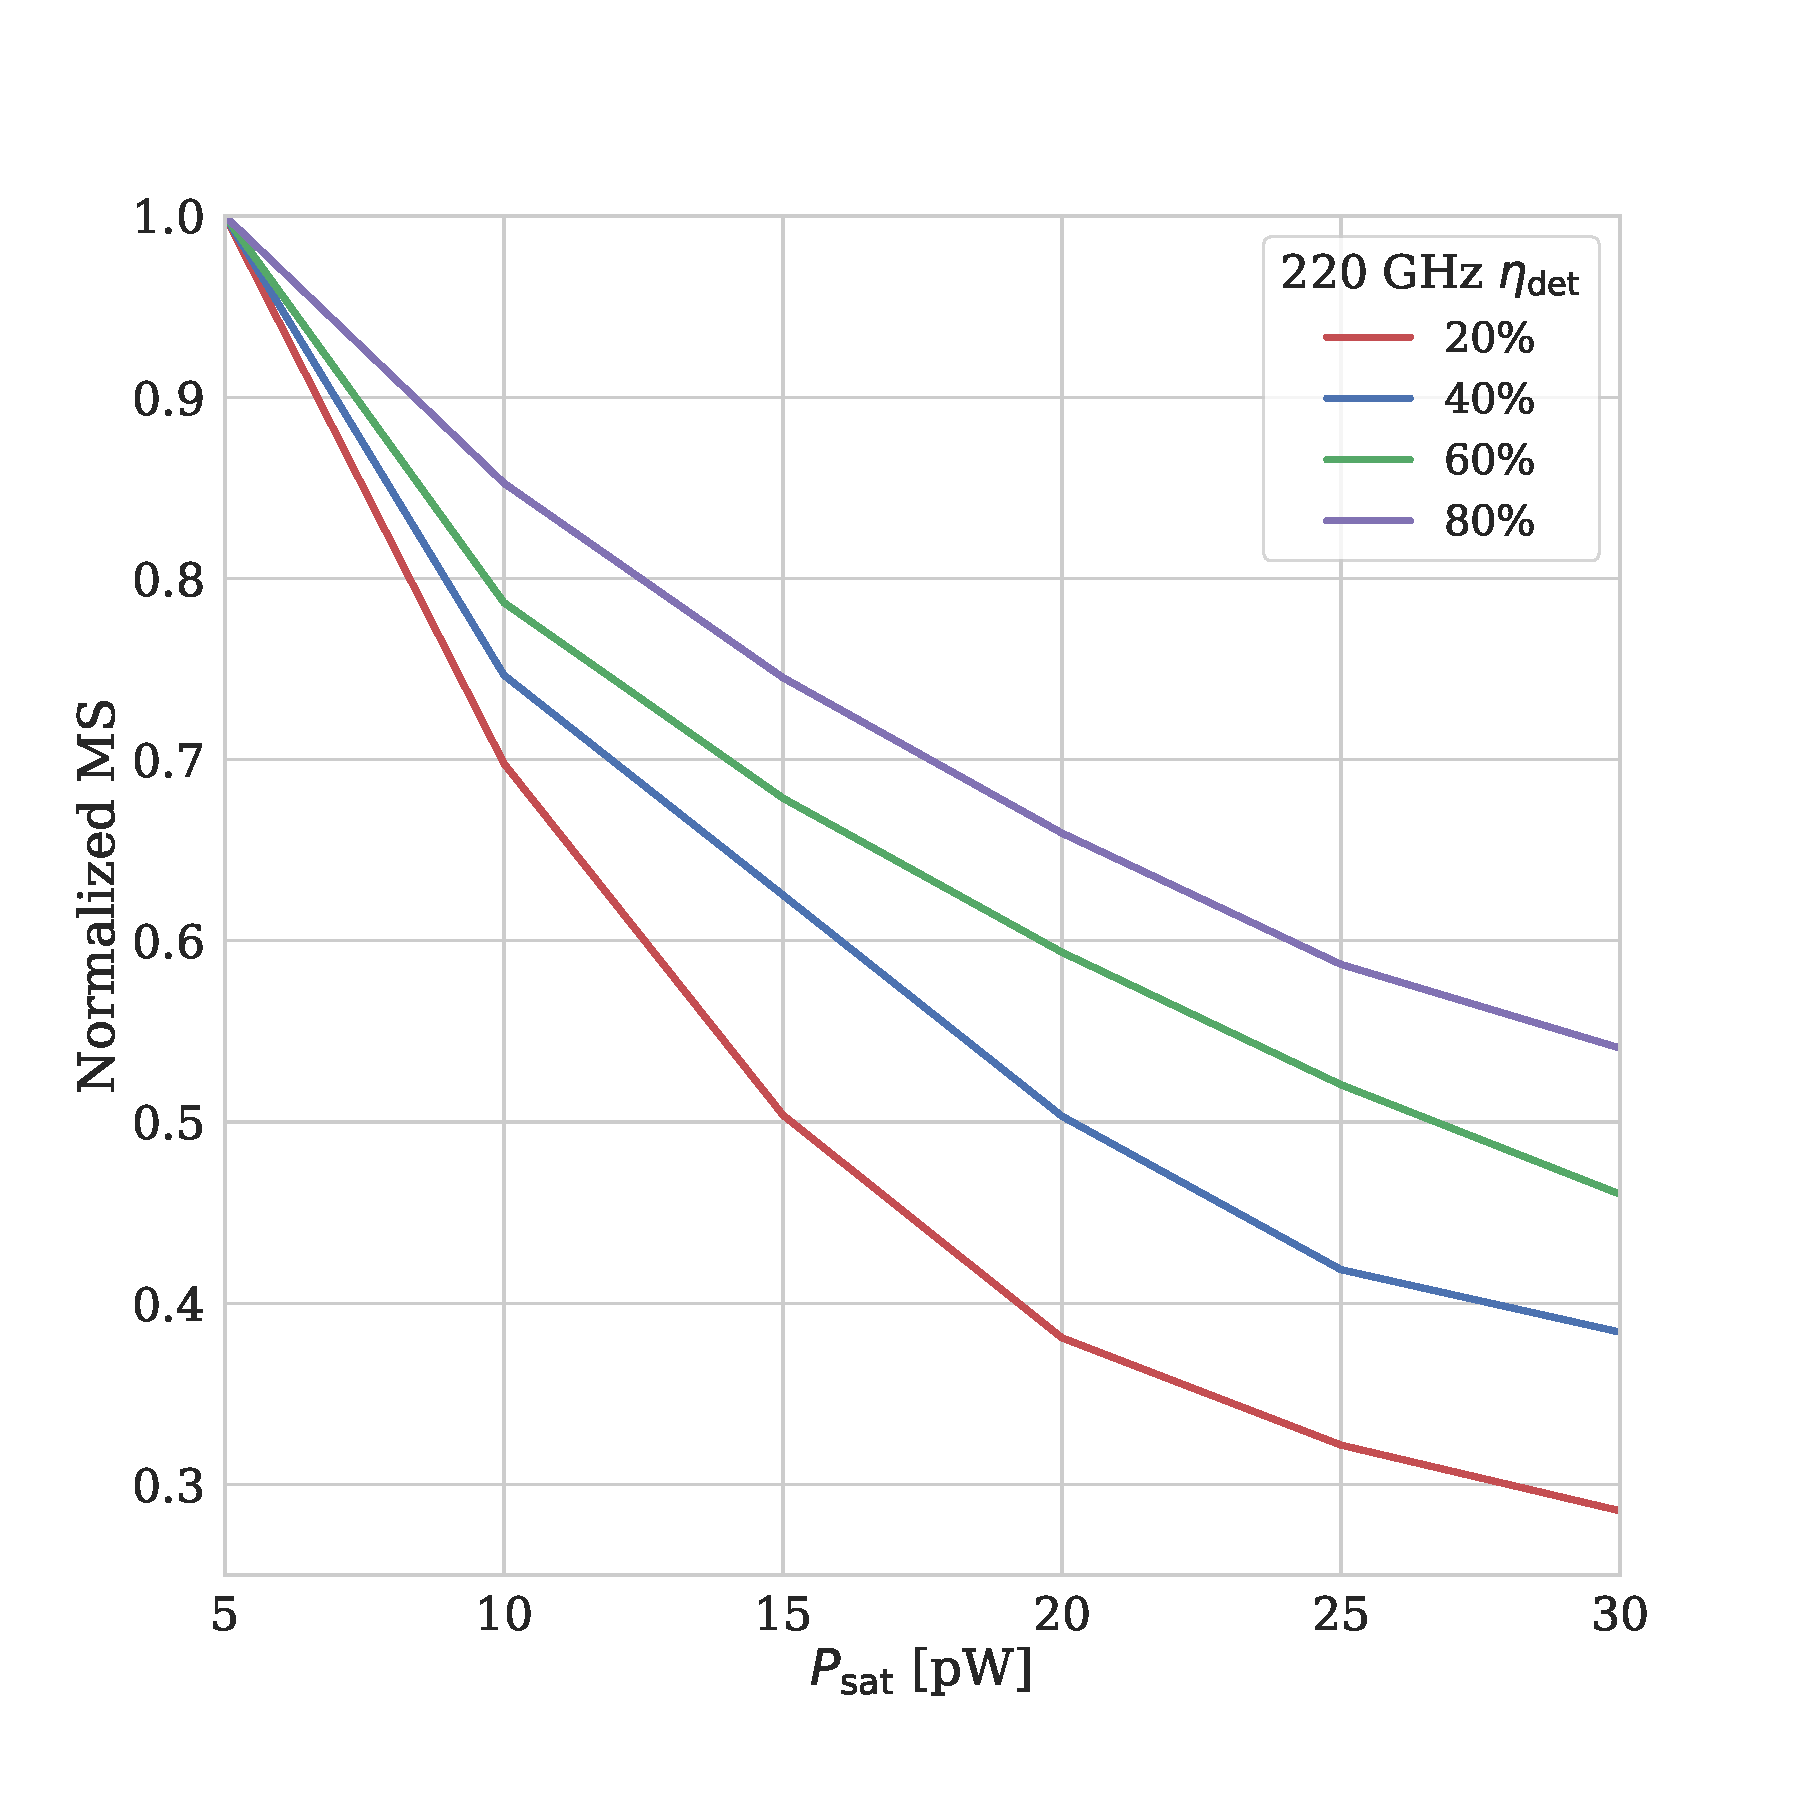
\includegraphics[width=0.48\linewidth, trim=0cm 0cm 0cm 0cm, clip]{BoloCalc/Figures/220_Psat_MS_allEffs.pdf}}
    \subfloat[\label{fig:pb2c_psat_ms:b}]{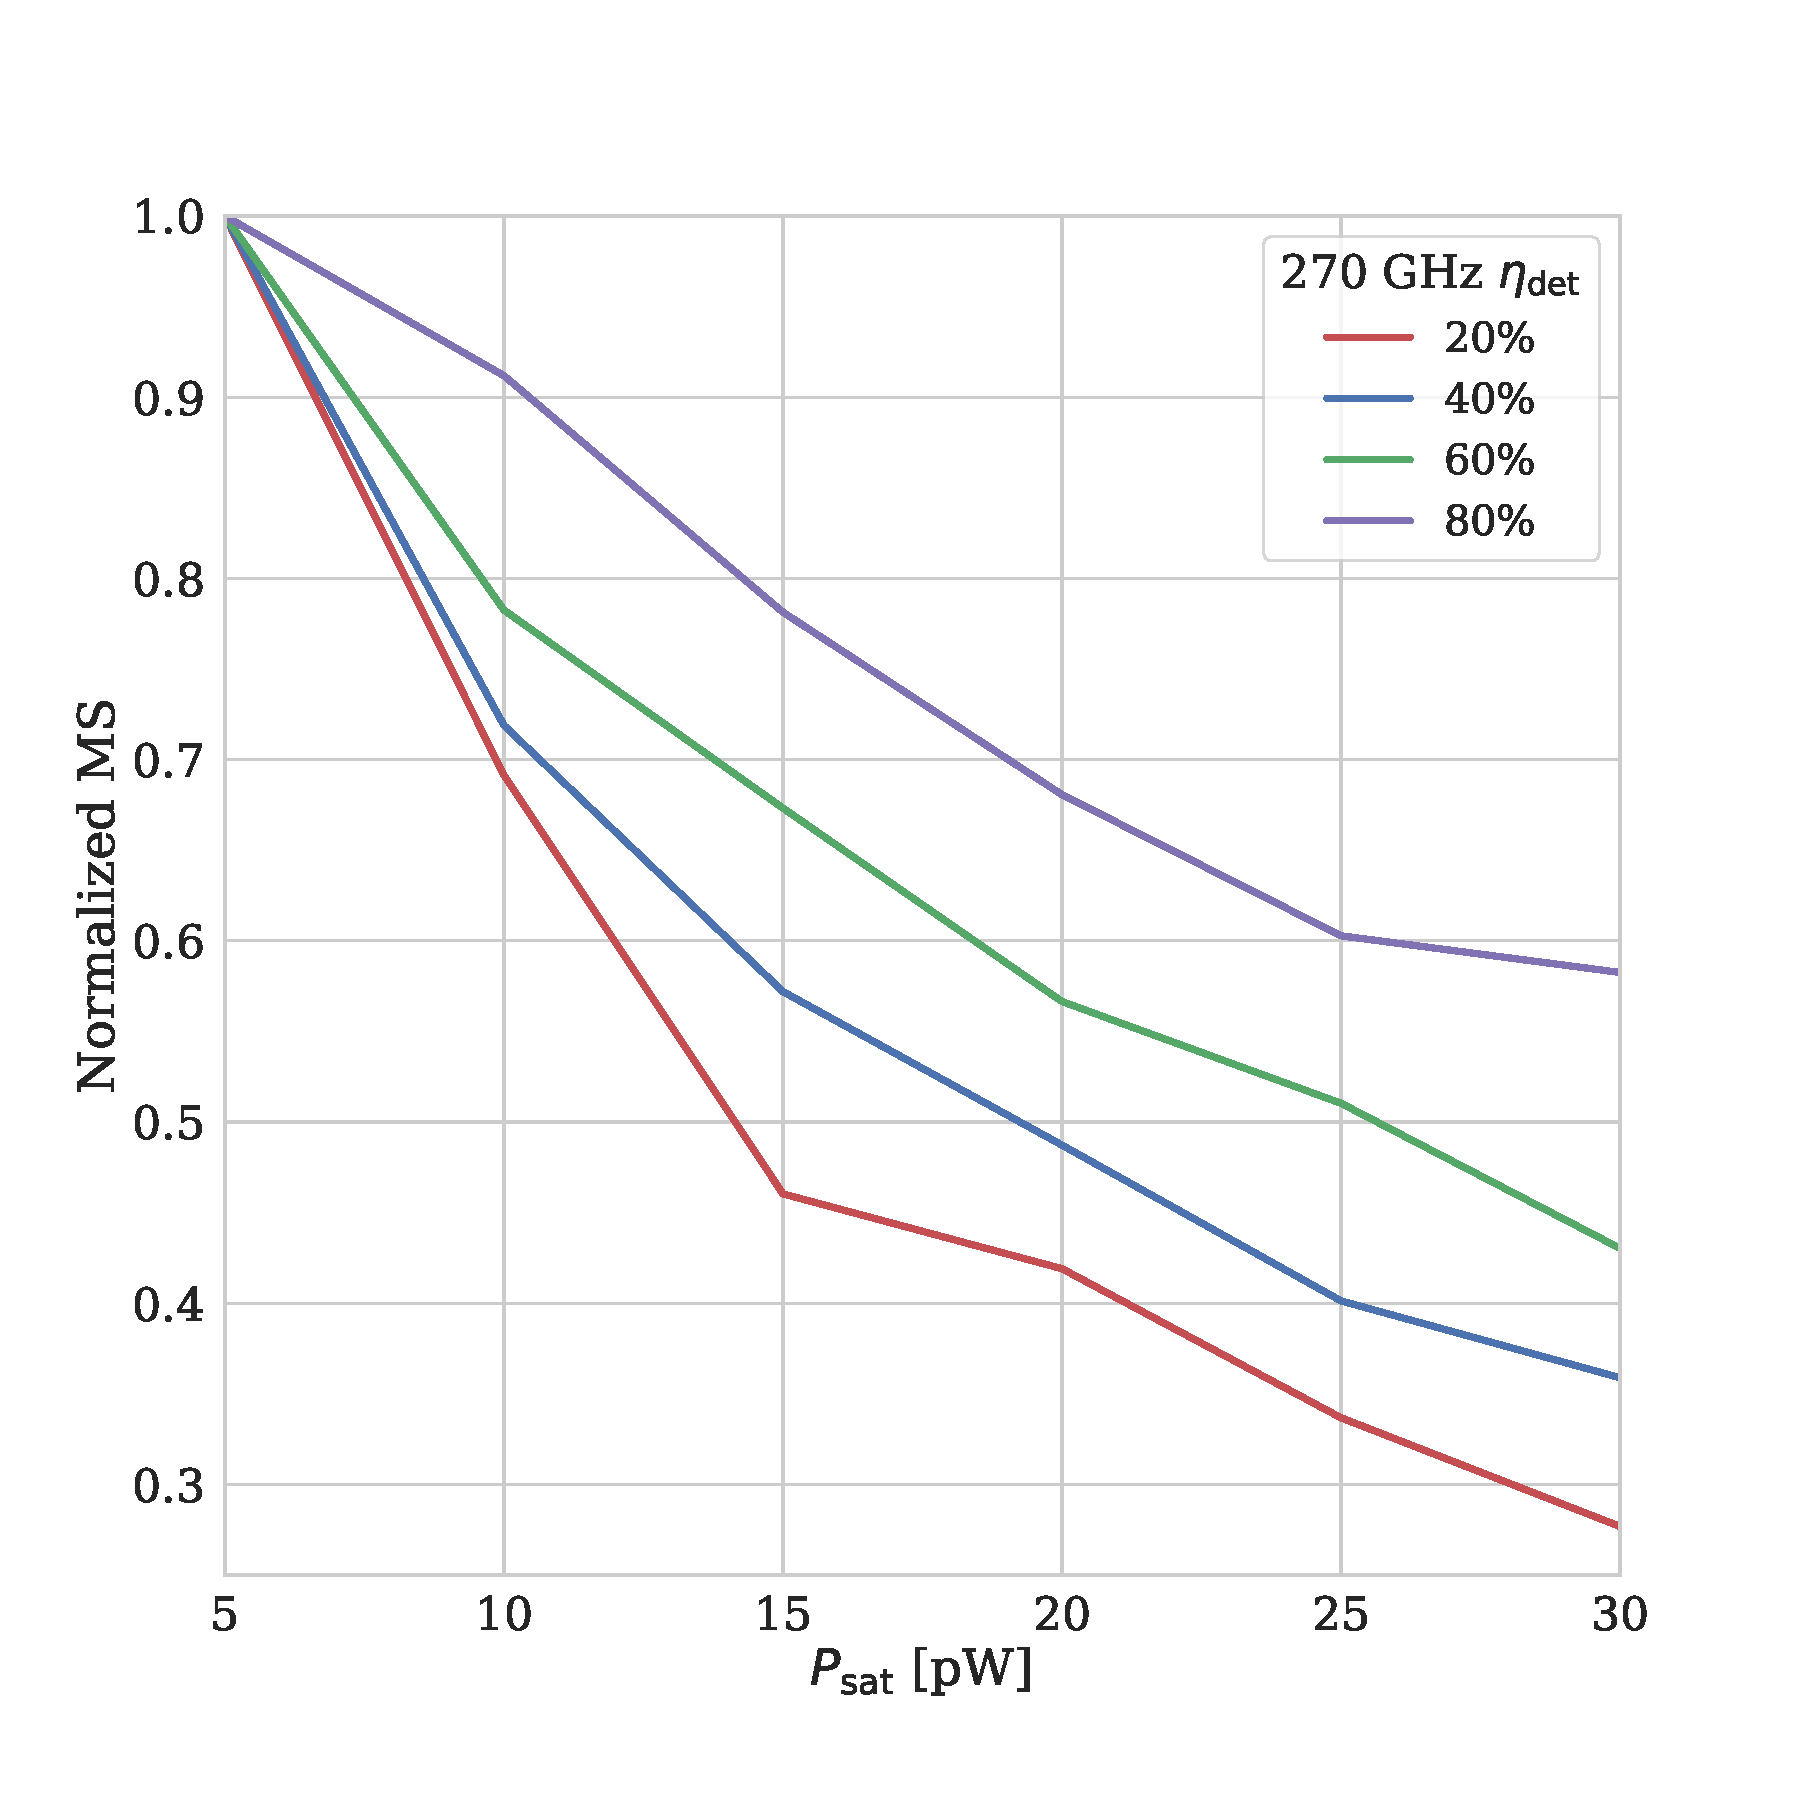
\includegraphics[width=0.48\linewidth, trim=0cm 0cm 0cm 0cm, clip]{BoloCalc/Figures/270_Psat_MS_allEffs.pdf}}
    \caption{Mapping speed vs detector saturation power $P_{\mathrm{sat}}$ in the PB-2c 220 and 270~GHz, normalized to $P_{\mathrm{sat}} = 5$~pW. The impact of $P_{\mathrm{sat}}$ is more pronounced with detector efficiency $\eta_{\mathrm{det}}$ is small, as the relative contrubtions of bolometer thermal carrier noise $\mathrm{NEP_{g}}$ and readout noise $\mathrm{NEP_{read}}$ to the total detector NEP increases with decreasing photon noise $\mathrm{NEP_{ph}}$ (see Equation~\ref{eq:nep_det}).}
    \label{fig:pb2c_psat_ms}
\end{figure}

To quantify the impact of $P_{\mathrm{sat}}$ on observation efficiency $\eta_{\mathrm{obs}}$, we must decide on a \important{$P_{\mathrm{opt}}$ cutoff}, or an optical load above which the telescope will not observe,\footnote{There are practical inputs such weather-driven decisions, such as the fact that it's ill-advised to observe in falling snow, but such extraneous factors tend to only arise at larger PWVs than those considered by this analysis.} which is in turn used to find $\eta_{\mathrm{obs}}$ from the cumulative probabilities in Figure~\ref{fig:pb2c_popt_cdf}. Such a decision is driven by detector saturation considerations, or when $P_{\mathrm{opt}}$ becomes large enough with respect to $P_{\mathrm{bias}}$ that the bolometer acts non-linearly or even becomes unstable. We can define this cutoff power in terms of $P_{\mathrm{sat}}$ as
\begin{equation}
    P_{\mathrm{cut}} \equiv \mathrm{MIN}\left[ \frac{P_{\mathrm{sat}}}{P_{\mathrm{opt}}} \right] \, .
    \label{eq:psat_cutoff}
\end{equation}
$P_{\mathrm{cut}}$ is analogous to \important{PWV cutoff} in that it corresponds to a sky temperature $T_{\mathrm{sky}}$ above which the instrument does not observe given some realization of the telescope load $T_{\mathrm{tel}}$ and some $P_{\mathrm{sat}}$. 
Armed with a functional dependence of mapping speed and observational efficiency on saturation power, we now plot $\mathrm{MS} \times \eta_{\mathrm{obs}}$ for various $\eta{\mathrm{det}}$ and $P_{\mathrm{cut}}$ in Figure~\ref{fig:pb2c_psat_ms_obsEff}.

There are features of the $\mathrm{MS} \times \eta_{\mathrm{obs}}$ optimization that are worth highlighting. First, lower $P_{\mathrm{sat}}$ is favored for lower $P_{\mathrm{cut}}$. This is the expected behavior given the proportionality relation in Equation~\ref{eq:psat_cutoff}. Second, the $P_{\mathrm{sat}}$ that maximizes sensitilvity is lower for lower $\eta_{\mathrm{det}}$. This too is expected, as $P_{\mathrm{opt}} \propto \eta_{\mathrm{det}}$. Third, the mapping-speed penalty of fielding a higer $P_{\mathrm{sat}}$ than is necessary is most pronounced at lower $P_{\mathrm{cut}}$ and lower $\eta_{\mathrm{det}}$. This is because total NEP becomes increasingly photon-noise dominated with increasing $\eta_{\mathrm{det}}$, and when the $\mathrm{NEP_{ph}}$ is substantially larger than $\mathrm{NEP_{g}}$ and $\mathrm{NEP_{read}}$, the importance of $P_{\mathrm{sat}}$ on NET is less pronounced, therefore loosening its tolerance. Fourth, along a similar vein, the larger the smaller the $P_{\mathrm{cut}}$, the more $T_{\mathrm{sky}}$ scenarios you allow yourself to observe in, in turn allowing a broader range of $P_{\mathrm{sat}}$ values to be ``viable.'' This phenomenon is most clearly seen when contrasting highest and lowest $P_{\mathrm{cut}}$ values. The $P_{\mathrm{cut}} = 2$ case asserts that the bolometer bias must satisfy $P_{\mathrm{bias}} \geq P_{\mathrm{opt}}$, and in this case, for all $\eta_{\mathrm{det}}$, if the $P_{\mathrm{sat}} \leq 10$~pW, the detector is inoperable in \textit{any} sky-loading scenario. However, if the same bolometers are fielded and the cutoff requirement is relaxed to $P_{\mathrm{cut}} = 1.25$, then all of a sudden bolometers with $P_{\mathrm{sat}} = 10$~pW become optimal (in the $\eta_{\mathrm{det}} =$~(40, 60)\% cases). In reality, $P_{\mathrm{cut}}$ is determined in-situ, after learning about how the responsivitiy of the detector array scales with $P_{\mathrm{bias}}$ in the field. In the limit of a large $\dd R_{\mathrm{bolo}} / \dd T_{\mathrm{bolo}}$, the open loop gain $\mathcal{L} \gg 1$, and responsivities are maximized. However, if $\dd R_{\mathrm{bolo}} / \dd T_{\mathrm{bolo}}$ is shallow, then $\mathcal{L} \propto P_{\mathrm{bias}}$, and maintaining a larger $P_{\mathrm{bias}} / P_{\mathrm{opt}}$ ratio could be important for bolometer linearity. Hence, this analysis is performed for various $P_{\mathrm{cut}}$ values to help understand the dependence of $\mathrm{MS} \times \eta_{\mathrm{obs}}$ on it.

\begin{figure}[!t]
    \centering
    \subfloat[\label{fig:pb2c_psat_ms_obsEff:a}]{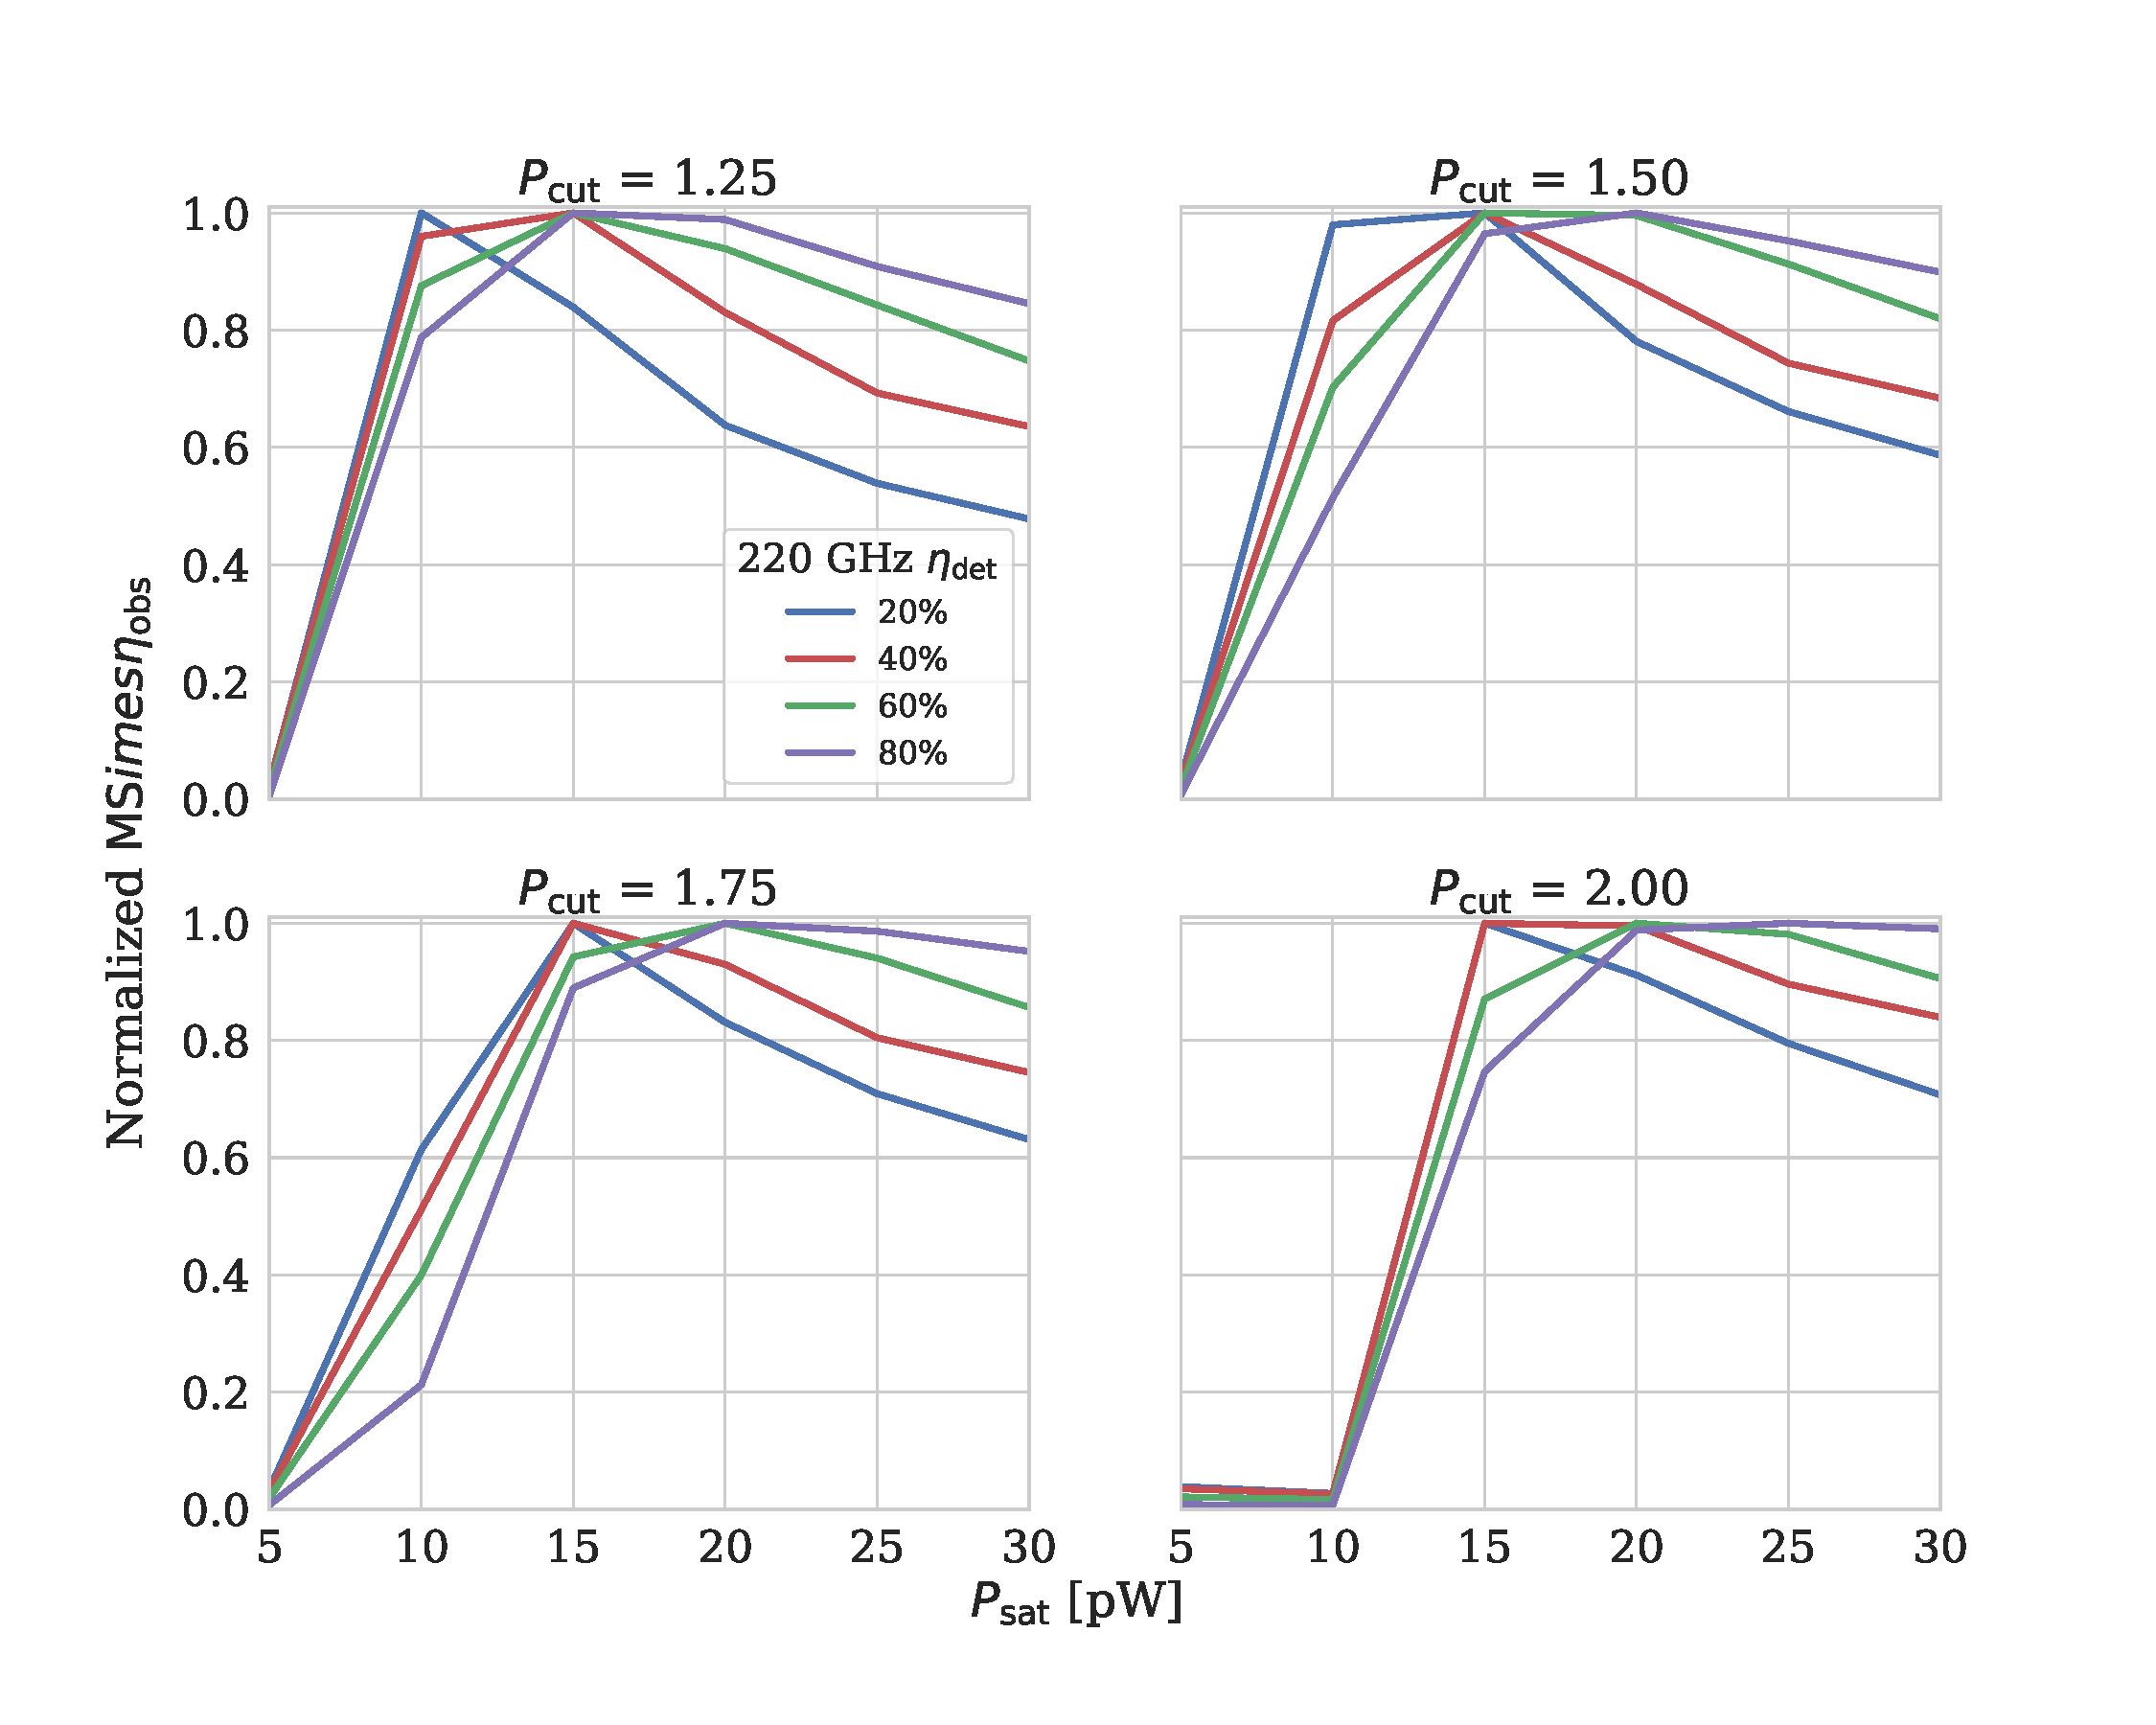
\includegraphics[width=0.48\linewidth, trim=1cm 1cm 1cm 1cm, clip]{BoloCalc/Figures/220_Psat_MS_obsEff.pdf}}
    %\hfill
    \subfloat[\label{fig:pb2c_psat_ms_obsEff:b}]{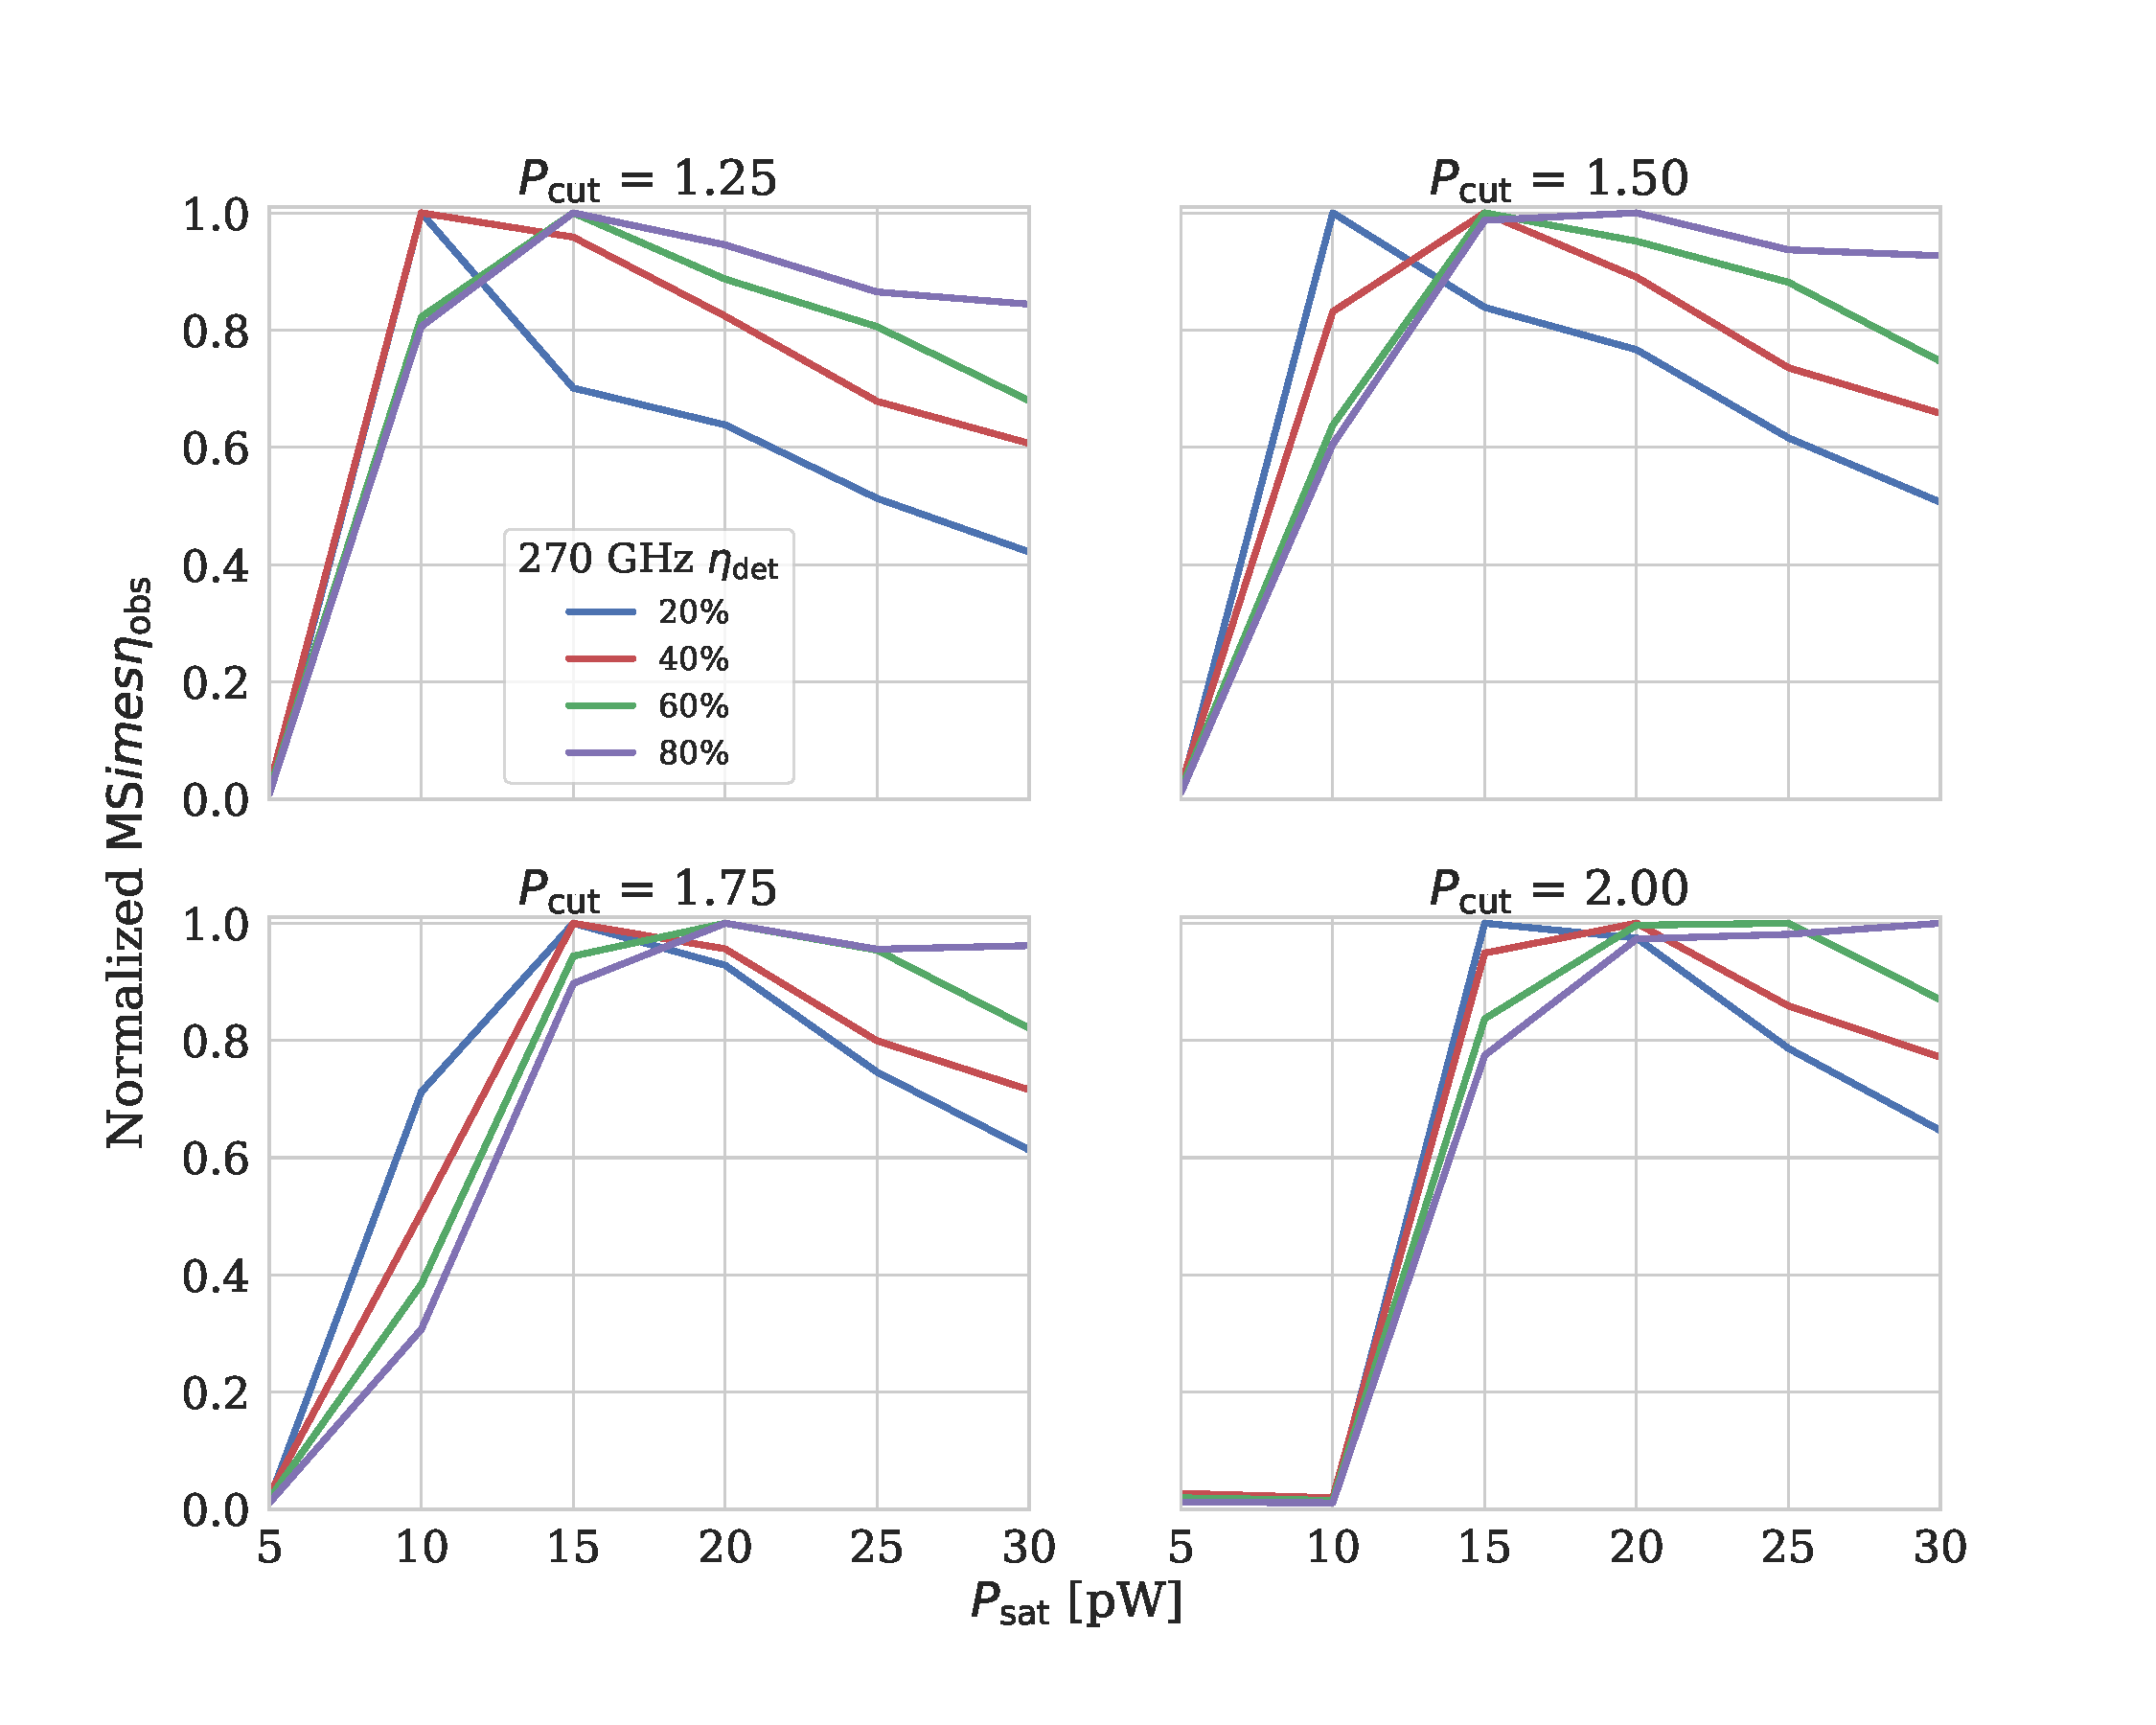
\includegraphics[width=0.48\linewidth, trim=1cm 1cm 1cm 1cm, clip]{BoloCalc/Figures/270_Psat_MS_obsEff.pdf}}
    \caption{Peak-normalized mapping speed MS vs detector saturation power $P_{\mathrm{sat}}$ in the PB-2c 220 and 270~GHz bands for various $P_{\mathrm{sat}}$ cutoffs $P_{\mathrm{cut}}$ (see Equation~\ref{eq:psat_cutoff}) and detector optical efficiencies $\eta{\mathrm{det}}$. The impact of deploying bolometers with overly conservative saturation powers is most pronounced at low $P_{\mathrm{cut}}$ and high $\eta_{\mathrm{det}}$.}
    \label{fig:pb2c_psat_ms_obsEff}
\end{figure}

The presented study was critically important to assign $P_{\mathrm{sat}}$ targets for PB-2c bolometers and to assess the viability of fabricated detectors for deployment. In addition, it is a useful demonstration of how BoloCalc can be used to optimize the detector array during late-stage instrument development.

%%%%%%%%%%%%%%%%%%%%%%%%%%%%%%%%
%%%%%%%%%%%%%%%%%%%%%%%%%%%%%%%%
%%%%%%%%%%%%%%%%%%%%%%%%%%%%%%%%

\section{Other applications}
\label{sec:bolocal_other_applications}

In this chapter, we have presented the design and application of BoloCalc within SA and SO. However, the sensitivity calculator's impact is much larger than with the presented research. 

BoloCalc was originally conceived and first used to inform the detector array design for LiteBIRD (LB), a Japanese-funded next-generation CMB satellite experiment whose mission is to map the entire sky from 40 to 400~GHz. In order characterize foregrounds with unprecedented precision, LB is deploying 15 observation bands within two separate on-board telescopes, and therefore optimizing the focal plane to achieve groundbreaking constraints on both cosmological parameters and inflationary gravitational waves was a major undertaking in the early stages. BoloCalc was at the heart of these efforts, generating a new 70-page ``sensitivity memo'' every few weeks as the instrument design evolved rapidly. Given this experience, BoloCalc has demonstrated applicability to CMB satellite missions and could be a useful tool for upcoming space-based observatories.

\begin{figure}
    \centering
    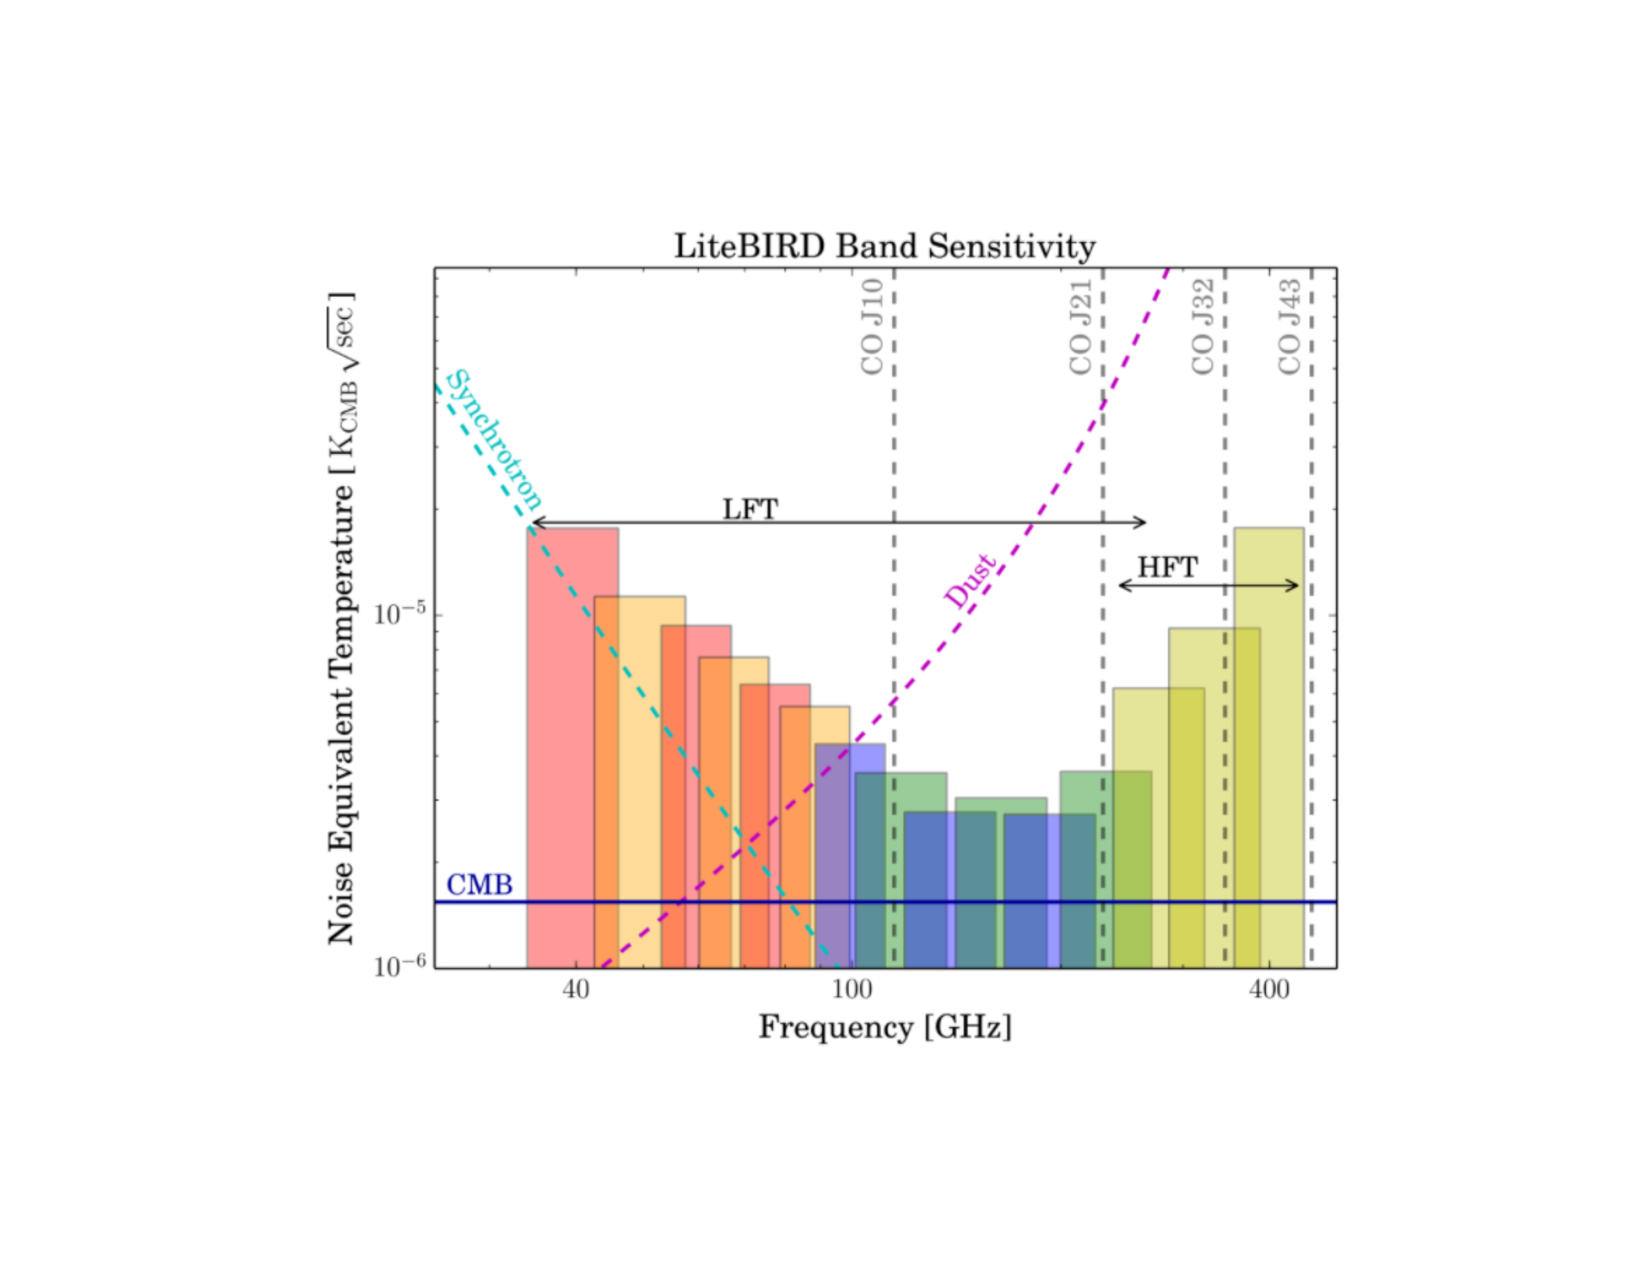
\includegraphics[width=0.7\linewidth, trim=5cm 3.5cm 5cm 3.5cm, clip]{BoloCalc/Figures/LiteBIRD_sensitivity.pdf}
    \caption{The distribution of bands and sensitivities for an early-stage incarnation (2016) of the LiteBIRD focal plane, as calculated by BoloCalc. The lower 12 bands are located in the low-frequency telescope (LFT), and the top three bands are located in the high-frequency telescope (HFT). Each detector pixel in the LFT is tri-chroic and is labeled with a distinct color. The y-axis is in units of $K_{\mathrm{CMB}}$, and the frequency dependence of synchrotron and dust emission are plotted with amplitudes that highlight the foreground minimum at $\approx$~70~GHz. The carbon-monoxide (CO) emission lines are only slightly polarized but are very bright and therefore are relegated to one band per line, avoiding overlapping band regions. Since this figure was made, the distribution of bands between telescopes and the projected sensitivities have changed, but the importance of this initial study continues to resonate through LiteBIRD's instrument design and mission concept.}
    \label{fig:litebird_bands}
\end{figure}

In addition, BoloCalc is making its way into other experiments as well, both within the CMB and outside of it. It has been used for as part of optical studies for BLAST, a far-IR balloon-borne telescope, and has been used as part of a cross-correlation feasibility study between 21-cm cosmology experiments and SO. Finally, the ultimate goal of BoloCalc is to be of use to the upcoming Department of Energy-funded CMB-Stage 4 (CMB-S4), which will turn a 300~million dollar budget into the ultimate ground-based measurement of CMB temperature and polarization anisotropies. In a similar way to SO, CMB-S4 will bring together many institutions, and therefore having a standardized, user-friendly, utilitarian sensitivity code will be essential to evaluate and advance the instrument design. Therefore, we hope that the calculator development presented in this dissertation will carry forward into the next generation of CMB experimentation and beyond.